\chapter{Notebook completo utilizado para la creación del sistema de recomendación}\label{app:notebook}

\section{\texorpdfstring{\textbf{Film recommendation
engine}}{Film recommendation engine}}\label{film-recommendation-engine}

\emph{Gonzalo Izaguirre (diciembre 2019)} \_\_\_

El objetivo de este notebook es crear un motor de recomendación a partir
del contenido del fichero \texttt{movie\_metadata.csv}.Este dataset
contiene alrededor de 5000 películas y series, y su descripción ha sido
recogida de la base de datos de IMDB. Basicamente, el sistema funcionará
de la siguiente forma: después de que el usuario haya introducido el
nombre de una película que le haya gustado, el sistema seleccionará del
conjunto total 5 películas que agradarán al usuario al ser similares.
This dataset contains around 5000 movies and TV series, and their
description has been retrieved from the public IMDB database. Existen
tres tipos de filtros colaborativos: - Sistemas
\textbf{popularity-based}: los más simples de implementar, aunque los
más impersonales - Sistemas \textbf{content-based}: La recomendación se
basa en la descripción del producto - Sistemas \textbf{collaborative
filtering}: datos de diferentes usuarios dan recomendaciones basadas en
similaridades entre usuarios.

In the current case, since the dataset only describe the content of the
films and TV series, collaborative filtering is excluded and I will thus
build an engine that uses both the content and the popularity of the
entries.

En este caso, dado que el conjunto de datos solo describe el contenido
de las películas, no puede aplicarse el filtrado colaborativo. Se creará
un motor que usará tanto el contenido como la popularidad de las
entradas. \_\_\_ El notebook se organiza de la siguiente manera:

\textbf{1. Exploración} - 1.1 Keywords - 1.2 Factor de completitud:
Valores Faltantes - 1.3 Géneros

\textbf{2. Limpieza} - 2.1 Entradas duplicadas - 2.2 Limpieza de
keywords * 2.2.1 Agrupamiento por lexema * 2.2.2 Agrupamiento por
sinónimos - 2.3 Correlaciones - 2.4 Valores faltantes * 2.4.1 Años
faltantes * 2.4.2 Extrayendo keywords del título * 2.4.3 Completado de
datos mediante regresión

\textbf{3. Recommendation Engine} - 3.1 Funcionamiento básico del motor
* 3.1.1 Similaridad * 3.1.2 Popularidad - 3.2 Definicion de las
funciones del motor de recomendación - 3.3 Realizando recomendaciones
interesantes - 3.4 Ejemplo de recomendación

\textbf{4. Conclusión: posibles mejoras y puntos a concretar}

    \begin{center}\rule{0.5\linewidth}{\linethickness}\end{center}

\subsection{1. Exploración}\label{exploraciuxf3n}

Se cargan todos los paquetes y el conjunto de datos. Se da información
sobre los tipos de las columnas y los datos faltantes.

    \begin{tcolorbox}[breakable, size=fbox, boxrule=1pt, pad at break*=1mm,colback=cellbackground, colframe=cellborder]
\prompt{In}{incolor}{1}{\hspace{4pt}}
\begin{Verbatim}[commandchars=\\\{\}]
\PY{k+kn}{import} \PY{n+nn}{json}
\PY{k+kn}{import} \PY{n+nn}{pandas} \PY{k}{as} \PY{n+nn}{pd}
\end{Verbatim}
\end{tcolorbox}

    \begin{tcolorbox}[breakable, size=fbox, boxrule=1pt, pad at break*=1mm,colback=cellbackground, colframe=cellborder]
\prompt{In}{incolor}{2}{\hspace{4pt}}
\begin{Verbatim}[commandchars=\\\{\}]
\PY{k}{def} \PY{n+nf}{load\PYZus{}movies}\PY{p}{(}\PY{n}{path}\PY{p}{)}\PY{p}{:}
    \PY{l+s+sd}{\PYZdq{}\PYZdq{}\PYZdq{}Función utilizada para cargar el dataset de las películas. Se transforma a fecha el campo de fecha de salida}
\PY{l+s+sd}{    y se cargan como listas los campos que están guardados como json.}
\PY{l+s+sd}{    }
\PY{l+s+sd}{    Args:}
\PY{l+s+sd}{        path (str): Ruta hasta el archivo de tmdb\PYZus{}5000\PYZus{}movies.csv}
\PY{l+s+sd}{    }
\PY{l+s+sd}{    Returns:}
\PY{l+s+sd}{        pd.DataFrame: Dataframe de pandas con la información del csv}
\PY{l+s+sd}{    \PYZdq{}\PYZdq{}\PYZdq{}}
    \PY{n}{df} \PY{o}{=} \PY{n}{pd}\PY{o}{.}\PY{n}{read\PYZus{}csv}\PY{p}{(}\PY{n}{path}\PY{p}{)}
    \PY{n}{df}\PY{p}{[}\PY{l+s+s1}{\PYZsq{}}\PY{l+s+s1}{release\PYZus{}date}\PY{l+s+s1}{\PYZsq{}}\PY{p}{]} \PY{o}{=} \PY{n}{pd}\PY{o}{.}\PY{n}{to\PYZus{}datetime}\PY{p}{(}\PY{n}{df}\PY{p}{[}\PY{l+s+s1}{\PYZsq{}}\PY{l+s+s1}{release\PYZus{}date}\PY{l+s+s1}{\PYZsq{}}\PY{p}{]}\PY{p}{)}\PY{o}{.}\PY{n}{apply}\PY{p}{(}\PY{k}{lambda} \PY{n}{x}\PY{p}{:} \PY{n}{x}\PY{o}{.}\PY{n}{date}\PY{p}{(}\PY{p}{)}\PY{p}{)}
    \PY{n}{json\PYZus{}columns} \PY{o}{=} \PY{p}{[}\PY{l+s+s1}{\PYZsq{}}\PY{l+s+s1}{genres}\PY{l+s+s1}{\PYZsq{}}\PY{p}{,} \PY{l+s+s1}{\PYZsq{}}\PY{l+s+s1}{keywords}\PY{l+s+s1}{\PYZsq{}}\PY{p}{,} \PY{l+s+s1}{\PYZsq{}}\PY{l+s+s1}{production\PYZus{}countries}\PY{l+s+s1}{\PYZsq{}}\PY{p}{,} \PY{l+s+s1}{\PYZsq{}}\PY{l+s+s1}{production\PYZus{}companies}\PY{l+s+s1}{\PYZsq{}}\PY{p}{,} \PY{l+s+s1}{\PYZsq{}}\PY{l+s+s1}{spoken\PYZus{}languages}\PY{l+s+s1}{\PYZsq{}}\PY{p}{]}
    \PY{k}{for} \PY{n}{column} \PY{o+ow}{in} \PY{n}{json\PYZus{}columns}\PY{p}{:}
        \PY{n}{df}\PY{p}{[}\PY{n}{column}\PY{p}{]} \PY{o}{=} \PY{n}{df}\PY{p}{[}\PY{n}{column}\PY{p}{]}\PY{o}{.}\PY{n}{apply}\PY{p}{(}\PY{n}{json}\PY{o}{.}\PY{n}{loads}\PY{p}{)}
    \PY{k}{return} \PY{n}{df}


\PY{k}{def} \PY{n+nf}{load\PYZus{}credits}\PY{p}{(}\PY{n}{path}\PY{p}{)}\PY{p}{:}
    \PY{l+s+sd}{\PYZdq{}\PYZdq{}\PYZdq{}Función utilizada para cargar el dataset de los créditos. Se cargan como listas los campos que están guardado}
\PY{l+s+sd}{    }
\PY{l+s+sd}{    Args:}
\PY{l+s+sd}{        path (str): Ruta hasta el archivo de tmdb\PYZus{}5000\PYZus{}credits.csv}

\PY{l+s+sd}{    Returns:}
\PY{l+s+sd}{        pd.DataFrame: [description]}
\PY{l+s+sd}{    \PYZdq{}\PYZdq{}\PYZdq{}}
    \PY{n}{df} \PY{o}{=} \PY{n}{pd}\PY{o}{.}\PY{n}{read\PYZus{}csv}\PY{p}{(}\PY{n}{path}\PY{p}{)}
    \PY{n}{json\PYZus{}columns} \PY{o}{=} \PY{p}{[}\PY{l+s+s1}{\PYZsq{}}\PY{l+s+s1}{cast}\PY{l+s+s1}{\PYZsq{}}\PY{p}{,} \PY{l+s+s1}{\PYZsq{}}\PY{l+s+s1}{crew}\PY{l+s+s1}{\PYZsq{}}\PY{p}{]}
    \PY{k}{for} \PY{n}{column} \PY{o+ow}{in} \PY{n}{json\PYZus{}columns}\PY{p}{:}
        \PY{n}{df}\PY{p}{[}\PY{n}{column}\PY{p}{]} \PY{o}{=} \PY{n}{df}\PY{p}{[}\PY{n}{column}\PY{p}{]}\PY{o}{.}\PY{n}{apply}\PY{p}{(}\PY{n}{json}\PY{o}{.}\PY{n}{loads}\PY{p}{)}
    \PY{k}{return} \PY{n}{df}
\end{Verbatim}
\end{tcolorbox}

    \begin{tcolorbox}[breakable, size=fbox, boxrule=1pt, pad at break*=1mm,colback=cellbackground, colframe=cellborder]
\prompt{In}{incolor}{3}{\hspace{4pt}}
\begin{Verbatim}[commandchars=\\\{\}]
\PY{n}{TMDB\PYZus{}TO\PYZus{}IMDB\PYZus{}SIMPLE\PYZus{}EQUIVALENCIES} \PY{o}{=} \PY{p}{\PYZob{}}
    \PY{l+s+s1}{\PYZsq{}}\PY{l+s+s1}{budget}\PY{l+s+s1}{\PYZsq{}}\PY{p}{:} \PY{l+s+s1}{\PYZsq{}}\PY{l+s+s1}{budget}\PY{l+s+s1}{\PYZsq{}}\PY{p}{,}
    \PY{l+s+s1}{\PYZsq{}}\PY{l+s+s1}{genres}\PY{l+s+s1}{\PYZsq{}}\PY{p}{:} \PY{l+s+s1}{\PYZsq{}}\PY{l+s+s1}{genres}\PY{l+s+s1}{\PYZsq{}}\PY{p}{,}
    \PY{l+s+s1}{\PYZsq{}}\PY{l+s+s1}{revenue}\PY{l+s+s1}{\PYZsq{}}\PY{p}{:} \PY{l+s+s1}{\PYZsq{}}\PY{l+s+s1}{gross}\PY{l+s+s1}{\PYZsq{}}\PY{p}{,}
    \PY{l+s+s1}{\PYZsq{}}\PY{l+s+s1}{title}\PY{l+s+s1}{\PYZsq{}}\PY{p}{:} \PY{l+s+s1}{\PYZsq{}}\PY{l+s+s1}{movie\PYZus{}title}\PY{l+s+s1}{\PYZsq{}}\PY{p}{,}
    \PY{l+s+s1}{\PYZsq{}}\PY{l+s+s1}{runtime}\PY{l+s+s1}{\PYZsq{}}\PY{p}{:} \PY{l+s+s1}{\PYZsq{}}\PY{l+s+s1}{duration}\PY{l+s+s1}{\PYZsq{}}\PY{p}{,}
    \PY{l+s+s1}{\PYZsq{}}\PY{l+s+s1}{original\PYZus{}language}\PY{l+s+s1}{\PYZsq{}}\PY{p}{:} \PY{l+s+s1}{\PYZsq{}}\PY{l+s+s1}{language}\PY{l+s+s1}{\PYZsq{}}\PY{p}{,}  \PY{c+c1}{\PYZsh{} it\PYZsq{}s possible that spoken\PYZus{}languages would be a better match}
    \PY{l+s+s1}{\PYZsq{}}\PY{l+s+s1}{keywords}\PY{l+s+s1}{\PYZsq{}}\PY{p}{:} \PY{l+s+s1}{\PYZsq{}}\PY{l+s+s1}{plot\PYZus{}keywords}\PY{l+s+s1}{\PYZsq{}}\PY{p}{,}
    \PY{l+s+s1}{\PYZsq{}}\PY{l+s+s1}{vote\PYZus{}count}\PY{l+s+s1}{\PYZsq{}}\PY{p}{:} \PY{l+s+s1}{\PYZsq{}}\PY{l+s+s1}{num\PYZus{}voted\PYZus{}users}\PY{l+s+s1}{\PYZsq{}}\PY{p}{,}
                                         \PY{p}{\PYZcb{}}

\PY{n}{IMDB\PYZus{}COLUMNS\PYZus{}TO\PYZus{}REMAP} \PY{o}{=} \PY{p}{\PYZob{}}\PY{l+s+s1}{\PYZsq{}}\PY{l+s+s1}{imdb\PYZus{}score}\PY{l+s+s1}{\PYZsq{}}\PY{p}{:} \PY{l+s+s1}{\PYZsq{}}\PY{l+s+s1}{vote\PYZus{}average}\PY{l+s+s1}{\PYZsq{}}\PY{p}{\PYZcb{}}
\end{Verbatim}
\end{tcolorbox}

    \begin{tcolorbox}[breakable, size=fbox, boxrule=1pt, pad at break*=1mm,colback=cellbackground, colframe=cellborder]
\prompt{In}{incolor}{4}{\hspace{4pt}}
\begin{Verbatim}[commandchars=\\\{\}]
\PY{o}{\PYZpc{}}\PY{k}{config} IPCompleter.greedy=True
\end{Verbatim}
\end{tcolorbox}

    \begin{tcolorbox}[breakable, size=fbox, boxrule=1pt, pad at break*=1mm,colback=cellbackground, colframe=cellborder]
\prompt{In}{incolor}{5}{\hspace{4pt}}
\begin{Verbatim}[commandchars=\\\{\}]
\PY{k}{def} \PY{n+nf}{get\PYZus{}element}\PY{p}{(}\PY{n}{container}\PY{p}{,} \PY{n}{index\PYZus{}values}\PY{p}{)}\PY{p}{:}
    \PY{l+s+sd}{\PYZdq{}\PYZdq{}\PYZdq{}Función para acceder de forma segura a valores. En caso de que no se encuentre uno de ellos, se devuelve NaN}
\PY{l+s+sd}{    en vez de lanzar un error.}
\PY{l+s+sd}{    }
\PY{l+s+sd}{    Args:}
\PY{l+s+sd}{        container (list): Lista/ contenedor de la que quieren extraerse los valores}
\PY{l+s+sd}{        index\PYZus{}values (list): Lista de índices a extraer del contenedor}
\PY{l+s+sd}{    }
\PY{l+s+sd}{    Returns:}
\PY{l+s+sd}{        any: Valores extraidos}
\PY{l+s+sd}{    \PYZdq{}\PYZdq{}\PYZdq{}}
    \PY{n}{result} \PY{o}{=} \PY{n}{container}
    \PY{k}{try}\PY{p}{:}
        \PY{k}{for} \PY{n}{idx} \PY{o+ow}{in} \PY{n}{index\PYZus{}values}\PY{p}{:}
            \PY{n}{result} \PY{o}{=} \PY{n}{result}\PY{p}{[}\PY{n}{idx}\PY{p}{]}
        \PY{k}{return} \PY{n}{result}
    \PY{k}{except} \PY{n+ne}{IndexError} \PY{o+ow}{or} \PY{n+ne}{KeyError}\PY{p}{:}
        \PY{k}{return} \PY{n}{pd}\PY{o}{.}\PY{n}{np}\PY{o}{.}\PY{n}{nan}


\PY{k}{def} \PY{n+nf}{get\PYZus{}director}\PY{p}{(}\PY{n}{crew\PYZus{}data}\PY{p}{)}\PY{p}{:}
    \PY{l+s+sd}{\PYZdq{}\PYZdq{}\PYZdq{}Devuelve el director dado un json con toda la composición del equipo de la película.}
\PY{l+s+sd}{    }
\PY{l+s+sd}{    Args:}
\PY{l+s+sd}{        crew\PYZus{}data (json): JSON con el equipo que ha realizado la película}
\PY{l+s+sd}{    }
\PY{l+s+sd}{    Returns:}
\PY{l+s+sd}{        str: Director de la película}
\PY{l+s+sd}{    \PYZdq{}\PYZdq{}\PYZdq{}}
    \PY{n}{directors} \PY{o}{=} \PY{p}{[}\PY{n}{x}\PY{p}{[}\PY{l+s+s1}{\PYZsq{}}\PY{l+s+s1}{name}\PY{l+s+s1}{\PYZsq{}}\PY{p}{]} \PY{k}{for} \PY{n}{x} \PY{o+ow}{in} \PY{n}{crew\PYZus{}data} \PY{k}{if} \PY{n}{x}\PY{p}{[}\PY{l+s+s1}{\PYZsq{}}\PY{l+s+s1}{job}\PY{l+s+s1}{\PYZsq{}}\PY{p}{]} \PY{o}{==} \PY{l+s+s1}{\PYZsq{}}\PY{l+s+s1}{Director}\PY{l+s+s1}{\PYZsq{}}\PY{p}{]}
    \PY{k}{return} \PY{n}{get\PYZus{}element}\PY{p}{(}\PY{n}{directors}\PY{p}{,} \PY{p}{[}\PY{l+m+mi}{0}\PY{p}{]}\PY{p}{)}


\PY{k}{def} \PY{n+nf}{flatten\PYZus{}names}\PY{p}{(}\PY{n}{keywords}\PY{p}{)}\PY{p}{:}
    \PY{l+s+sd}{\PYZdq{}\PYZdq{}\PYZdq{}Obtiene una lista con las keywords separadas por un pipe | extrayéndolas del json.}
\PY{l+s+sd}{    }
\PY{l+s+sd}{    Args:}
\PY{l+s+sd}{        keywords (json): keywords de la película}
\PY{l+s+sd}{    }
\PY{l+s+sd}{    Returns:}
\PY{l+s+sd}{        str: keywords de la película juntas}
\PY{l+s+sd}{    \PYZdq{}\PYZdq{}\PYZdq{}}
    \PY{k}{return} \PY{l+s+s1}{\PYZsq{}}\PY{l+s+s1}{|}\PY{l+s+s1}{\PYZsq{}}\PY{o}{.}\PY{n}{join}\PY{p}{(}\PY{p}{[}\PY{n}{x}\PY{p}{[}\PY{l+s+s1}{\PYZsq{}}\PY{l+s+s1}{name}\PY{l+s+s1}{\PYZsq{}}\PY{p}{]} \PY{k}{for} \PY{n}{x} \PY{o+ow}{in} \PY{n}{keywords}\PY{p}{]}\PY{p}{)}


\PY{k}{def} \PY{n+nf}{combine\PYZus{}collections}\PY{p}{(}\PY{n}{movies}\PY{p}{,} \PY{n}{credits}\PY{p}{)}\PY{p}{:}
    \PY{l+s+sd}{\PYZdq{}\PYZdq{}\PYZdq{}Aplica una serie de funciones para añadir información al dataset de películas a partir del}
\PY{l+s+sd}{    conjunto de datos de créditos}
\PY{l+s+sd}{    }
\PY{l+s+sd}{    Args:}
\PY{l+s+sd}{        movies (pd.DataFrame): DataFrame obtenido de leer el archivo de películas}
\PY{l+s+sd}{        credits (pd.DataFrame): DataFrame obtenido de leet el archivo de créditos}
\PY{l+s+sd}{    }
\PY{l+s+sd}{    Returns:}
\PY{l+s+sd}{        pd.DataFrame: DataFrame con la información conjunta}
\PY{l+s+sd}{    \PYZdq{}\PYZdq{}\PYZdq{}}
    \PY{n}{tmdb\PYZus{}movies} \PY{o}{=} \PY{n}{movies}\PY{o}{.}\PY{n}{copy}\PY{p}{(}\PY{p}{)}
    \PY{n}{tmdb\PYZus{}movies}\PY{o}{.}\PY{n}{rename}\PY{p}{(}\PY{n}{columns}\PY{o}{=}\PY{n}{TMDB\PYZus{}TO\PYZus{}IMDB\PYZus{}SIMPLE\PYZus{}EQUIVALENCIES}\PY{p}{,} \PY{n}{inplace}\PY{o}{=}\PY{k+kc}{True}\PY{p}{)}
    \PY{n}{tmdb\PYZus{}movies}\PY{p}{[}\PY{l+s+s1}{\PYZsq{}}\PY{l+s+s1}{title\PYZus{}year}\PY{l+s+s1}{\PYZsq{}}\PY{p}{]} \PY{o}{=} \PY{n}{pd}\PY{o}{.}\PY{n}{to\PYZus{}datetime}\PY{p}{(}\PY{n}{tmdb\PYZus{}movies}\PY{p}{[}\PY{l+s+s1}{\PYZsq{}}\PY{l+s+s1}{release\PYZus{}date}\PY{l+s+s1}{\PYZsq{}}\PY{p}{]}\PY{p}{)}\PY{o}{.}\PY{n}{apply}\PY{p}{(}\PY{k}{lambda} \PY{n}{x}\PY{p}{:} \PY{n}{x}\PY{o}{.}\PY{n}{year}\PY{p}{)}
    \PY{c+c1}{\PYZsh{} I\PYZsq{}m assuming that the first production country is equivalent, but have not been able to validate this}
    \PY{n}{tmdb\PYZus{}movies}\PY{p}{[}\PY{l+s+s1}{\PYZsq{}}\PY{l+s+s1}{country}\PY{l+s+s1}{\PYZsq{}}\PY{p}{]} \PY{o}{=} \PY{n}{tmdb\PYZus{}movies}\PY{p}{[}\PY{l+s+s1}{\PYZsq{}}\PY{l+s+s1}{production\PYZus{}countries}\PY{l+s+s1}{\PYZsq{}}\PY{p}{]}\PY{o}{.}\PY{n}{apply}\PY{p}{(}\PY{k}{lambda} \PY{n}{x}\PY{p}{:} \PY{n}{get\PYZus{}element}\PY{p}{(}\PY{n}{x}\PY{p}{,} \PY{p}{[}\PY{l+m+mi}{0}\PY{p}{,} \PY{l+s+s1}{\PYZsq{}}\PY{l+s+s1}{name}\PY{l+s+s1}{\PYZsq{}}\PY{p}{]}\PY{p}{)}\PY{p}{)}
    \PY{n}{tmdb\PYZus{}movies}\PY{p}{[}\PY{l+s+s1}{\PYZsq{}}\PY{l+s+s1}{language}\PY{l+s+s1}{\PYZsq{}}\PY{p}{]} \PY{o}{=} \PY{n}{tmdb\PYZus{}movies}\PY{p}{[}\PY{l+s+s1}{\PYZsq{}}\PY{l+s+s1}{spoken\PYZus{}languages}\PY{l+s+s1}{\PYZsq{}}\PY{p}{]}\PY{o}{.}\PY{n}{apply}\PY{p}{(}\PY{k}{lambda} \PY{n}{x}\PY{p}{:} \PY{n}{get\PYZus{}element}\PY{p}{(}\PY{n}{x}\PY{p}{,} \PY{p}{[}\PY{l+m+mi}{0}\PY{p}{,} \PY{l+s+s1}{\PYZsq{}}\PY{l+s+s1}{name}\PY{l+s+s1}{\PYZsq{}}\PY{p}{]}\PY{p}{)}\PY{p}{)}
    \PY{n}{tmdb\PYZus{}movies}\PY{p}{[}\PY{l+s+s1}{\PYZsq{}}\PY{l+s+s1}{director\PYZus{}name}\PY{l+s+s1}{\PYZsq{}}\PY{p}{]} \PY{o}{=} \PY{n}{credits}\PY{p}{[}\PY{l+s+s1}{\PYZsq{}}\PY{l+s+s1}{crew}\PY{l+s+s1}{\PYZsq{}}\PY{p}{]}\PY{o}{.}\PY{n}{apply}\PY{p}{(}\PY{n}{get\PYZus{}director}\PY{p}{)}
    \PY{n}{tmdb\PYZus{}movies}\PY{p}{[}\PY{l+s+s1}{\PYZsq{}}\PY{l+s+s1}{actor\PYZus{}1\PYZus{}name}\PY{l+s+s1}{\PYZsq{}}\PY{p}{]} \PY{o}{=} \PY{n}{credits}\PY{p}{[}\PY{l+s+s1}{\PYZsq{}}\PY{l+s+s1}{cast}\PY{l+s+s1}{\PYZsq{}}\PY{p}{]}\PY{o}{.}\PY{n}{apply}\PY{p}{(}\PY{k}{lambda} \PY{n}{x}\PY{p}{:} \PY{n}{get\PYZus{}element}\PY{p}{(}\PY{n}{x}\PY{p}{,} \PY{p}{[}\PY{l+m+mi}{1}\PY{p}{,} \PY{l+s+s1}{\PYZsq{}}\PY{l+s+s1}{name}\PY{l+s+s1}{\PYZsq{}}\PY{p}{]}\PY{p}{)}\PY{p}{)}
    \PY{n}{tmdb\PYZus{}movies}\PY{p}{[}\PY{l+s+s1}{\PYZsq{}}\PY{l+s+s1}{actor\PYZus{}2\PYZus{}name}\PY{l+s+s1}{\PYZsq{}}\PY{p}{]} \PY{o}{=} \PY{n}{credits}\PY{p}{[}\PY{l+s+s1}{\PYZsq{}}\PY{l+s+s1}{cast}\PY{l+s+s1}{\PYZsq{}}\PY{p}{]}\PY{o}{.}\PY{n}{apply}\PY{p}{(}\PY{k}{lambda} \PY{n}{x}\PY{p}{:} \PY{n}{get\PYZus{}element}\PY{p}{(}\PY{n}{x}\PY{p}{,} \PY{p}{[}\PY{l+m+mi}{2}\PY{p}{,} \PY{l+s+s1}{\PYZsq{}}\PY{l+s+s1}{name}\PY{l+s+s1}{\PYZsq{}}\PY{p}{]}\PY{p}{)}\PY{p}{)}
    \PY{n}{tmdb\PYZus{}movies}\PY{p}{[}\PY{l+s+s1}{\PYZsq{}}\PY{l+s+s1}{actor\PYZus{}3\PYZus{}name}\PY{l+s+s1}{\PYZsq{}}\PY{p}{]} \PY{o}{=} \PY{n}{credits}\PY{p}{[}\PY{l+s+s1}{\PYZsq{}}\PY{l+s+s1}{cast}\PY{l+s+s1}{\PYZsq{}}\PY{p}{]}\PY{o}{.}\PY{n}{apply}\PY{p}{(}\PY{k}{lambda} \PY{n}{x}\PY{p}{:} \PY{n}{get\PYZus{}element}\PY{p}{(}\PY{n}{x}\PY{p}{,} \PY{p}{[}\PY{l+m+mi}{3}\PY{p}{,} \PY{l+s+s1}{\PYZsq{}}\PY{l+s+s1}{name}\PY{l+s+s1}{\PYZsq{}}\PY{p}{]}\PY{p}{)}\PY{p}{)}
    \PY{n}{tmdb\PYZus{}movies}\PY{p}{[}\PY{l+s+s1}{\PYZsq{}}\PY{l+s+s1}{genres}\PY{l+s+s1}{\PYZsq{}}\PY{p}{]} \PY{o}{=} \PY{n}{tmdb\PYZus{}movies}\PY{p}{[}\PY{l+s+s1}{\PYZsq{}}\PY{l+s+s1}{genres}\PY{l+s+s1}{\PYZsq{}}\PY{p}{]}\PY{o}{.}\PY{n}{apply}\PY{p}{(}\PY{n}{flatten\PYZus{}names}\PY{p}{)}
    \PY{n}{tmdb\PYZus{}movies}\PY{p}{[}\PY{l+s+s1}{\PYZsq{}}\PY{l+s+s1}{plot\PYZus{}keywords}\PY{l+s+s1}{\PYZsq{}}\PY{p}{]} \PY{o}{=} \PY{n}{tmdb\PYZus{}movies}\PY{p}{[}\PY{l+s+s1}{\PYZsq{}}\PY{l+s+s1}{plot\PYZus{}keywords}\PY{l+s+s1}{\PYZsq{}}\PY{p}{]}\PY{o}{.}\PY{n}{apply}\PY{p}{(}\PY{n}{flatten\PYZus{}names}\PY{p}{)}
    \PY{k}{return} \PY{n}{tmdb\PYZus{}movies}
\end{Verbatim}
\end{tcolorbox}

    \begin{tcolorbox}[breakable, size=fbox, boxrule=1pt, pad at break*=1mm,colback=cellbackground, colframe=cellborder]
\prompt{In}{incolor}{6}{\hspace{4pt}}
\begin{Verbatim}[commandchars=\\\{\}]
\PY{k+kn}{import} \PY{n+nn}{pandas} \PY{k}{as} \PY{n+nn}{pd}
\PY{k+kn}{import} \PY{n+nn}{numpy} \PY{k}{as} \PY{n+nn}{np}
\PY{k+kn}{import} \PY{n+nn}{matplotlib} \PY{k}{as} \PY{n+nn}{mpl}
\PY{k+kn}{import} \PY{n+nn}{matplotlib}\PY{n+nn}{.}\PY{n+nn}{pyplot} \PY{k}{as} \PY{n+nn}{plt}
\PY{k+kn}{import} \PY{n+nn}{seaborn} \PY{k}{as} \PY{n+nn}{sns}
\PY{k+kn}{import} \PY{n+nn}{math}\PY{o}{,} \PY{n+nn}{nltk}\PY{o}{,} \PY{n+nn}{warnings}
\PY{k+kn}{from} \PY{n+nn}{nltk}\PY{n+nn}{.}\PY{n+nn}{corpus} \PY{k+kn}{import} \PY{n}{wordnet}
\PY{k+kn}{from} \PY{n+nn}{sklearn} \PY{k+kn}{import} \PY{n}{linear\PYZus{}model}
\PY{k+kn}{from} \PY{n+nn}{sklearn}\PY{n+nn}{.}\PY{n+nn}{neighbors} \PY{k+kn}{import} \PY{n}{NearestNeighbors}
\PY{k+kn}{from} \PY{n+nn}{fuzzywuzzy} \PY{k+kn}{import} \PY{n}{fuzz}
\PY{k+kn}{from} \PY{n+nn}{wordcloud} \PY{k+kn}{import} \PY{n}{WordCloud}\PY{p}{,} \PY{n}{STOPWORDS}
\PY{n}{plt}\PY{o}{.}\PY{n}{rcParams}\PY{p}{[}\PY{l+s+s2}{\PYZdq{}}\PY{l+s+s2}{patch.force\PYZus{}edgecolor}\PY{l+s+s2}{\PYZdq{}}\PY{p}{]} \PY{o}{=} \PY{k+kc}{True}
\PY{n}{plt}\PY{o}{.}\PY{n}{style}\PY{o}{.}\PY{n}{use}\PY{p}{(}\PY{l+s+s1}{\PYZsq{}}\PY{l+s+s1}{fivethirtyeight}\PY{l+s+s1}{\PYZsq{}}\PY{p}{)}
\PY{n}{mpl}\PY{o}{.}\PY{n}{rc}\PY{p}{(}\PY{l+s+s1}{\PYZsq{}}\PY{l+s+s1}{patch}\PY{l+s+s1}{\PYZsq{}}\PY{p}{,} \PY{n}{edgecolor} \PY{o}{=} \PY{l+s+s1}{\PYZsq{}}\PY{l+s+s1}{dimgray}\PY{l+s+s1}{\PYZsq{}}\PY{p}{,} \PY{n}{linewidth}\PY{o}{=}\PY{l+m+mi}{1}\PY{p}{)}
\PY{k+kn}{from} \PY{n+nn}{IPython}\PY{n+nn}{.}\PY{n+nn}{core}\PY{n+nn}{.}\PY{n+nn}{interactiveshell} \PY{k+kn}{import} \PY{n}{InteractiveShell}
\PY{n}{InteractiveShell}\PY{o}{.}\PY{n}{ast\PYZus{}node\PYZus{}interactivity} \PY{o}{=} \PY{l+s+s2}{\PYZdq{}}\PY{l+s+s2}{last\PYZus{}expr}\PY{l+s+s2}{\PYZdq{}}
\PY{n}{pd}\PY{o}{.}\PY{n}{options}\PY{o}{.}\PY{n}{display}\PY{o}{.}\PY{n}{max\PYZus{}columns} \PY{o}{=} \PY{l+m+mi}{50}
\PY{o}{\PYZpc{}}\PY{k}{matplotlib} inline
\PY{n}{warnings}\PY{o}{.}\PY{n}{filterwarnings}\PY{p}{(}\PY{l+s+s1}{\PYZsq{}}\PY{l+s+s1}{ignore}\PY{l+s+s1}{\PYZsq{}}\PY{p}{)}

\PY{c+c1}{\PYZsh{}Definimos la función a utilizar para obtener el lexema de las palabras.}
\PY{n}{PS} \PY{o}{=} \PY{n}{nltk}\PY{o}{.}\PY{n}{stem}\PY{o}{.}\PY{n}{PorterStemmer}\PY{p}{(}\PY{p}{)}
\PY{c+c1}{\PYZsh{}\PYZus{}\PYZus{}\PYZus{}\PYZus{}\PYZus{}\PYZus{}\PYZus{}\PYZus{}\PYZus{}\PYZus{}\PYZus{}\PYZus{}\PYZus{}\PYZus{}\PYZus{}\PYZus{}\PYZus{}\PYZus{}}
\PY{c+c1}{\PYZsh{} load the dataset}
\PY{c+c1}{\PYZsh{}df\PYZus{}initial = pd.read\PYZus{}csv(\PYZdq{}../input/movie\PYZus{}metadata.csv\PYZdq{})}
\PY{n}{credits} \PY{o}{=} \PY{n}{load\PYZus{}credits}\PY{p}{(}\PY{l+s+s2}{\PYZdq{}}\PY{l+s+s2}{../RecommendationEngine/datos/tmdb\PYZus{}5000\PYZus{}credits.csv}\PY{l+s+s2}{\PYZdq{}}\PY{p}{)}
\PY{n}{movies} \PY{o}{=} \PY{n}{load\PYZus{}movies}\PY{p}{(}\PY{l+s+s2}{\PYZdq{}}\PY{l+s+s2}{../RecommendationEngine/datos/tmdb\PYZus{}5000\PYZus{}movies.csv}\PY{l+s+s2}{\PYZdq{}}\PY{p}{)}
\PY{n}{df\PYZus{}initial} \PY{o}{=} \PY{n}{combine\PYZus{}collections}\PY{p}{(}\PY{n}{movies}\PY{p}{,} \PY{n}{credits}\PY{p}{)}
\PY{n+nb}{print}\PY{p}{(}\PY{l+s+s1}{\PYZsq{}}\PY{l+s+s1}{Shape:}\PY{l+s+s1}{\PYZsq{}}\PY{p}{,}\PY{n}{df\PYZus{}initial}\PY{o}{.}\PY{n}{shape}\PY{p}{)}
\PY{c+c1}{\PYZsh{}\PYZus{}\PYZus{}\PYZus{}\PYZus{}\PYZus{}\PYZus{}\PYZus{}\PYZus{}\PYZus{}\PYZus{}\PYZus{}\PYZus{}\PYZus{}\PYZus{}\PYZus{}\PYZus{}\PYZus{}\PYZus{}\PYZus{}\PYZus{}\PYZus{}\PYZus{}\PYZus{}\PYZus{}\PYZus{}\PYZus{}\PYZus{}\PYZus{}\PYZus{}\PYZus{}\PYZus{}\PYZus{}\PYZus{}\PYZus{}\PYZus{}\PYZus{}\PYZus{}\PYZus{}\PYZus{}\PYZus{}\PYZus{}\PYZus{}}
\PY{c+c1}{\PYZsh{} Información sobre los tipos de variable y el factor de completitud}
\PY{n}{tab\PYZus{}info}\PY{o}{=}\PY{n}{pd}\PY{o}{.}\PY{n}{DataFrame}\PY{p}{(}\PY{n}{df\PYZus{}initial}\PY{o}{.}\PY{n}{dtypes}\PY{p}{)}\PY{o}{.}\PY{n}{T}\PY{o}{.}\PY{n}{rename}\PY{p}{(}\PY{n}{index}\PY{o}{=}\PY{p}{\PYZob{}}\PY{l+m+mi}{0}\PY{p}{:}\PY{l+s+s1}{\PYZsq{}}\PY{l+s+s1}{column type}\PY{l+s+s1}{\PYZsq{}}\PY{p}{\PYZcb{}}\PY{p}{)}
\PY{n}{tab\PYZus{}info}\PY{o}{=}\PY{n}{tab\PYZus{}info}\PY{o}{.}\PY{n}{append}\PY{p}{(}\PY{n}{pd}\PY{o}{.}\PY{n}{DataFrame}\PY{p}{(}\PY{n}{df\PYZus{}initial}\PY{o}{.}\PY{n}{isnull}\PY{p}{(}\PY{p}{)}\PY{o}{.}\PY{n}{sum}\PY{p}{(}\PY{p}{)}\PY{p}{)}\PY{o}{.}\PY{n}{T}\PY{o}{.}\PY{n}{rename}\PY{p}{(}\PY{n}{index}\PY{o}{=}\PY{p}{\PYZob{}}\PY{l+m+mi}{0}\PY{p}{:}\PY{l+s+s1}{\PYZsq{}}\PY{l+s+s1}{null values}\PY{l+s+s1}{\PYZsq{}}\PY{p}{\PYZcb{}}\PY{p}{)}\PY{p}{)}
\PY{n}{tab\PYZus{}info}\PY{o}{=}\PY{n}{tab\PYZus{}info}\PY{o}{.}\PY{n}{append}\PY{p}{(}\PY{n}{pd}\PY{o}{.}\PY{n}{DataFrame}\PY{p}{(}\PY{n}{df\PYZus{}initial}\PY{o}{.}\PY{n}{isnull}\PY{p}{(}\PY{p}{)}\PY{o}{.}\PY{n}{sum}\PY{p}{(}\PY{p}{)}\PY{o}{/}\PY{n}{df\PYZus{}initial}\PY{o}{.}\PY{n}{shape}\PY{p}{[}\PY{l+m+mi}{0}\PY{p}{]}\PY{o}{*}\PY{l+m+mi}{100}\PY{p}{)}\PY{o}{.}\PY{n}{T}\PY{o}{.}
                         \PY{n}{rename}\PY{p}{(}\PY{n}{index}\PY{o}{=}\PY{p}{\PYZob{}}\PY{l+m+mi}{0}\PY{p}{:}\PY{l+s+s1}{\PYZsq{}}\PY{l+s+s1}{null values (}\PY{l+s+s1}{\PYZpc{}}\PY{l+s+s1}{)}\PY{l+s+s1}{\PYZsq{}}\PY{p}{\PYZcb{}}\PY{p}{)}\PY{p}{)}
\PY{n}{tab\PYZus{}info}
\end{Verbatim}
\end{tcolorbox}

    \begin{Verbatim}[commandchars=\\\{\}]
Shape: (4803, 26)
\end{Verbatim}

            \begin{tcolorbox}[breakable, boxrule=.5pt, size=fbox, pad at break*=1mm, opacityfill=0]
\prompt{Out}{outcolor}{6}{\hspace{3.5pt}}
\begin{Verbatim}[commandchars=\\\{\}]
                budget  genres homepage     id plot\_keywords language  \textbackslash{}
column type      int64  object   object  int64        object   object
null values          0       0     3091      0             0       86
null values (\%)      0       0  64.3556      0             0  1.79055

                original\_title  overview popularity production\_companies  \textbackslash{}
column type             object    object    float64               object
null values                  0         3          0                    0
null values (\%)              0  0.062461          0                    0

                production\_countries release\_date  gross   duration  \textbackslash{}
column type                   object       object  int64    float64
null values                        0            1      0          2
null values (\%)                    0    0.0208203      0  0.0416406

                spoken\_languages  status  tagline movie\_title vote\_average  \textbackslash{}
column type               object  object   object      object      float64
null values                    0       0      844           0            0
null values (\%)                0       0  17.5724           0            0

                num\_voted\_users title\_year  country director\_name  \textbackslash{}
column type               int64    float64   object        object
null values                   0          1      174            30
null values (\%)               0  0.0208203  3.62274       0.62461

                actor\_1\_name actor\_2\_name actor\_3\_name
column type           object       object       object
null values               53           63           93
null values (\%)      1.10348      1.31168      1.93629
\end{Verbatim}
\end{tcolorbox}
        
    \begin{tcolorbox}[breakable, size=fbox, boxrule=1pt, pad at break*=1mm,colback=cellbackground, colframe=cellborder]
\prompt{In}{incolor}{7}{\hspace{4pt}}
\begin{Verbatim}[commandchars=\\\{\}]
\PY{n+nb}{print}\PY{p}{(}\PY{n}{tab\PYZus{}info}\PY{o}{.}\PY{n}{to\PYZus{}latex}\PY{p}{(}\PY{p}{)}\PY{p}{)}
\end{Verbatim}
\end{tcolorbox}

    \begin{Verbatim}[commandchars=\\\{\}]
\textbackslash{}begin\{tabular\}\{lllllllllllllllllllllllllll\}
\textbackslash{}toprule
\{\} \& budget \&  genres \& homepage \&     id \& plot\textbackslash{}\_keywords \& language \&
original\textbackslash{}\_title \&  overview \& popularity \& production\textbackslash{}\_companies \&
production\textbackslash{}\_countries \& release\textbackslash{}\_date \&  gross \&   duration \& spoken\textbackslash{}\_languages
\&  status \&  tagline \& movie\textbackslash{}\_title \& vote\textbackslash{}\_average \& num\textbackslash{}\_voted\textbackslash{}\_users \&
title\textbackslash{}\_year \&  country \& director\textbackslash{}\_name \& actor\textbackslash{}\_1\textbackslash{}\_name \& actor\textbackslash{}\_2\textbackslash{}\_name \&
actor\textbackslash{}\_3\textbackslash{}\_name \textbackslash{}\textbackslash{}
\textbackslash{}midrule
column type     \&  int64 \&  object \&   object \&  int64 \&        object \&
object \&         object \&    object \&    float64 \&               object \&
object \&       object \&  int64 \&    float64 \&           object \&  object \&
object \&      object \&      float64 \&           int64 \&    float64 \&   object \&
object \&       object \&       object \&       object \textbackslash{}\textbackslash{}
null values     \&      0 \&       0 \&     3091 \&      0 \&             0 \&
86 \&              0 \&         3 \&          0 \&                    0 \&
0 \&            1 \&      0 \&          2 \&                0 \&       0 \&      844 \&
0 \&            0 \&               0 \&          1 \&      174 \&            30 \&
53 \&           63 \&           93 \textbackslash{}\textbackslash{}
null values (\textbackslash{}\%) \&      0 \&       0 \&  64.3556 \&      0 \&             0 \&
1.79055 \&              0 \&  0.062461 \&          0 \&                    0 \&
0 \&    0.0208203 \&      0 \&  0.0416406 \&                0 \&       0 \&  17.5724 \&
0 \&            0 \&               0 \&  0.0208203 \&  3.62274 \&       0.62461 \&
1.10348 \&      1.31168 \&      1.93629 \textbackslash{}\textbackslash{}
\textbackslash{}bottomrule
\textbackslash{}end\{tabular\}

\end{Verbatim}

    \begin{center}\rule{0.5\linewidth}{\linethickness}\end{center}

\subsubsection{1.1 Keywords}\label{keywords}

    Para desarrollar el sistema de recomendación, se hará un uso extensivo
de las palabras clave que describen las películas. De hecho, una
asunción básica en el proyecto es que las películas descritas por
keywords similares deberían tener contenido similar. Por tanto, se
realizará un analisis de cómo están definidas las keywords en un primer
paso. En primer lugar, veamos las keywords que hay en el conjunto de
datos.

    \begin{tcolorbox}[breakable, size=fbox, boxrule=1pt, pad at break*=1mm,colback=cellbackground, colframe=cellborder]
\prompt{In}{incolor}{8}{\hspace{4pt}}
\begin{Verbatim}[commandchars=\\\{\}]
\PY{n}{set\PYZus{}keywords} \PY{o}{=} \PY{n+nb}{set}\PY{p}{(}\PY{p}{)}
\PY{k}{for} \PY{n}{liste\PYZus{}keywords} \PY{o+ow}{in} \PY{n}{df\PYZus{}initial}\PY{p}{[}\PY{l+s+s1}{\PYZsq{}}\PY{l+s+s1}{plot\PYZus{}keywords}\PY{l+s+s1}{\PYZsq{}}\PY{p}{]}\PY{o}{.}\PY{n}{str}\PY{o}{.}\PY{n}{split}\PY{p}{(}\PY{l+s+s1}{\PYZsq{}}\PY{l+s+s1}{|}\PY{l+s+s1}{\PYZsq{}}\PY{p}{)}\PY{o}{.}\PY{n}{values}\PY{p}{:}
    \PY{k}{if} \PY{n+nb}{isinstance}\PY{p}{(}\PY{n}{liste\PYZus{}keywords}\PY{p}{,} \PY{n+nb}{float}\PY{p}{)}\PY{p}{:} \PY{k}{continue}  \PY{c+c1}{\PYZsh{} Evitar las películas en las que no hay keywords}
    \PY{n}{set\PYZus{}keywords} \PY{o}{=} \PY{n}{set\PYZus{}keywords}\PY{o}{.}\PY{n}{union}\PY{p}{(}\PY{n}{liste\PYZus{}keywords}\PY{p}{)}
\end{Verbatim}
\end{tcolorbox}

    and then define a function that counts the number of times each of them
appear:

    \begin{tcolorbox}[breakable, size=fbox, boxrule=1pt, pad at break*=1mm,colback=cellbackground, colframe=cellborder]
\prompt{In}{incolor}{9}{\hspace{4pt}}
\begin{Verbatim}[commandchars=\\\{\}]
\PY{k}{def} \PY{n+nf}{count\PYZus{}word}\PY{p}{(}\PY{n}{df}\PY{p}{,} \PY{n}{ref\PYZus{}col}\PY{p}{,} \PY{n}{lista}\PY{p}{)}\PY{p}{:}
    \PY{l+s+sd}{\PYZdq{}\PYZdq{}\PYZdq{}Toma una columna de un dataframe y un set de valores y devuelve un diccionario y una lista}
\PY{l+s+sd}{    con el numero de apariciones de cada elemento de la lista en la columna del dataframe}

\PY{l+s+sd}{    Args:}
\PY{l+s+sd}{        df (pd.DataFrame]): DataFrame del que extraer la información}
\PY{l+s+sd}{        ref\PYZus{}col (str): Columna de la que extraer los valores diferentes}
\PY{l+s+sd}{        lista (list): Lista con los diferentes valores de los que extraer sus apariciones}
\PY{l+s+sd}{    Returns:}
\PY{l+s+sd}{        list: Número de apariciones}
\PY{l+s+sd}{        dict: Número de apariciones}

\PY{l+s+sd}{    \PYZdq{}\PYZdq{}\PYZdq{}}
    \PY{n}{keyword\PYZus{}count} \PY{o}{=} \PY{n+nb}{dict}\PY{p}{(}\PY{p}{)}
    \PY{k}{for} \PY{n}{s} \PY{o+ow}{in} \PY{n}{lista}\PY{p}{:} \PY{n}{keyword\PYZus{}count}\PY{p}{[}\PY{n}{s}\PY{p}{]} \PY{o}{=} \PY{l+m+mi}{0}
    \PY{k}{for} \PY{n}{lista\PYZus{}keywords} \PY{o+ow}{in} \PY{n}{df}\PY{p}{[}\PY{n}{ref\PYZus{}col}\PY{p}{]}\PY{o}{.}\PY{n}{str}\PY{o}{.}\PY{n}{split}\PY{p}{(}\PY{l+s+s1}{\PYZsq{}}\PY{l+s+s1}{|}\PY{l+s+s1}{\PYZsq{}}\PY{p}{)}\PY{p}{:}
        \PY{k}{if} \PY{n+nb}{type}\PY{p}{(}\PY{n}{lista\PYZus{}keywords}\PY{p}{)} \PY{o}{==} \PY{n+nb}{float} \PY{o+ow}{and} \PY{n}{pd}\PY{o}{.}\PY{n}{isnull}\PY{p}{(}\PY{n}{lista\PYZus{}keywords}\PY{p}{)}\PY{p}{:} \PY{k}{continue}
        \PY{c+c1}{\PYZsh{}for s in lista:}
        \PY{k}{for} \PY{n}{s} \PY{o+ow}{in} \PY{p}{[}\PY{n}{s} \PY{k}{for} \PY{n}{s} \PY{o+ow}{in} \PY{n}{lista\PYZus{}keywords} \PY{k}{if} \PY{n}{s} \PY{o+ow}{in} \PY{n}{lista}\PY{p}{]}\PY{p}{:}
            \PY{k}{if} \PY{n}{pd}\PY{o}{.}\PY{n}{notnull}\PY{p}{(}\PY{n}{s}\PY{p}{)}\PY{p}{:} \PY{n}{keyword\PYZus{}count}\PY{p}{[}\PY{n}{s}\PY{p}{]} \PY{o}{+}\PY{o}{=} \PY{l+m+mi}{1}
    \PY{c+c1}{\PYZsh{}\PYZus{}\PYZus{}\PYZus{}\PYZus{}\PYZus{}\PYZus{}\PYZus{}\PYZus{}\PYZus{}\PYZus{}\PYZus{}\PYZus{}\PYZus{}\PYZus{}\PYZus{}\PYZus{}\PYZus{}\PYZus{}\PYZus{}\PYZus{}\PYZus{}\PYZus{}\PYZus{}\PYZus{}\PYZus{}\PYZus{}\PYZus{}\PYZus{}\PYZus{}\PYZus{}\PYZus{}\PYZus{}\PYZus{}\PYZus{}\PYZus{}\PYZus{}\PYZus{}\PYZus{}\PYZus{}\PYZus{}\PYZus{}\PYZus{}\PYZus{}\PYZus{}\PYZus{}\PYZus{}\PYZus{}\PYZus{}\PYZus{}\PYZus{}\PYZus{}\PYZus{}\PYZus{}\PYZus{}\PYZus{}\PYZus{}\PYZus{}\PYZus{}\PYZus{}\PYZus{}\PYZus{}\PYZus{}\PYZus{}\PYZus{}\PYZus{}\PYZus{}\PYZus{}\PYZus{}\PYZus{}\PYZus{}}
    \PY{c+c1}{\PYZsh{} convert the dictionary in a list to sort the keywords by frequency}
    \PY{n}{keyword\PYZus{}occurences} \PY{o}{=} \PY{p}{[}\PY{p}{]}
    \PY{k}{for} \PY{n}{k}\PY{p}{,}\PY{n}{v} \PY{o+ow}{in} \PY{n}{keyword\PYZus{}count}\PY{o}{.}\PY{n}{items}\PY{p}{(}\PY{p}{)}\PY{p}{:}
        \PY{n}{keyword\PYZus{}occurences}\PY{o}{.}\PY{n}{append}\PY{p}{(}\PY{p}{[}\PY{n}{k}\PY{p}{,}\PY{n}{v}\PY{p}{]}\PY{p}{)}
    \PY{n}{keyword\PYZus{}occurences}\PY{o}{.}\PY{n}{sort}\PY{p}{(}\PY{n}{key} \PY{o}{=} \PY{k}{lambda} \PY{n}{x}\PY{p}{:}\PY{n}{x}\PY{p}{[}\PY{l+m+mi}{1}\PY{p}{]}\PY{p}{,} \PY{n}{reverse} \PY{o}{=} \PY{k+kc}{True}\PY{p}{)}
    \PY{k}{return} \PY{n}{keyword\PYZus{}occurences}\PY{p}{,} \PY{n}{keyword\PYZus{}count}
\end{Verbatim}
\end{tcolorbox}

    Esta función se usará de nuevo en otras secciones del notebook, cuando
se explore el contenido de la variable \texttt{generos} y, obviamente,
cuando limpiemos las keywords. Finalmente, llamando a esta funcion
tenemos acceso a la lista de kweywords que están ordenadas en orden
decreciente por número de apariciones.

    \begin{tcolorbox}[breakable, size=fbox, boxrule=1pt, pad at break*=1mm,colback=cellbackground, colframe=cellborder]
\prompt{In}{incolor}{10}{\hspace{4pt}}
\begin{Verbatim}[commandchars=\\\{\}]
\PY{c+c1}{\PYZsh{} Diferentes keywords y número de apariciones}
\PY{n}{keyword\PYZus{}occurences}\PY{p}{,} \PY{n}{\PYZus{}} \PY{o}{=} \PY{n}{count\PYZus{}word}\PY{p}{(}\PY{n}{df\PYZus{}initial}\PY{p}{,} \PY{l+s+s1}{\PYZsq{}}\PY{l+s+s1}{plot\PYZus{}keywords}\PY{l+s+s1}{\PYZsq{}}\PY{p}{,} \PY{n}{set\PYZus{}keywords}\PY{p}{)}
\PY{n}{keyword\PYZus{}occurences}\PY{p}{[}\PY{p}{:}\PY{l+m+mi}{5}\PY{p}{]}
\end{Verbatim}
\end{tcolorbox}

            \begin{tcolorbox}[breakable, boxrule=.5pt, size=fbox, pad at break*=1mm, opacityfill=0]
\prompt{Out}{outcolor}{10}{\hspace{3.5pt}}
\begin{Verbatim}[commandchars=\\\{\}]
[['', 412],
 ['woman director', 324],
 ['independent film', 318],
 ['duringcreditsstinger', 307],
 ['based on novel', 197]]
\end{Verbatim}
\end{tcolorbox}
        
    \begin{tcolorbox}[breakable, size=fbox, boxrule=1pt, pad at break*=1mm,colback=cellbackground, colframe=cellborder]
\prompt{In}{incolor}{11}{\hspace{4pt}}
\begin{Verbatim}[commandchars=\\\{\}]
\PY{c+c1}{\PYZsh{} Se retiran las keywords que son vacías}
\PY{n}{keyword\PYZus{}occurences} \PY{o}{=} \PY{p}{[}\PY{n}{x} \PY{k}{for} \PY{n}{x} \PY{o+ow}{in} \PY{n}{keyword\PYZus{}occurences} \PY{k}{if} \PY{n}{x}\PY{p}{[}\PY{l+m+mi}{0}\PY{p}{]}\PY{p}{]}
\PY{n}{keyword\PYZus{}occurences}\PY{p}{[}\PY{p}{:}\PY{l+m+mi}{5}\PY{p}{]}
\end{Verbatim}
\end{tcolorbox}

            \begin{tcolorbox}[breakable, boxrule=.5pt, size=fbox, pad at break*=1mm, opacityfill=0]
\prompt{Out}{outcolor}{11}{\hspace{3.5pt}}
\begin{Verbatim}[commandchars=\\\{\}]
[['woman director', 324],
 ['independent film', 318],
 ['duringcreditsstinger', 307],
 ['based on novel', 197],
 ['murder', 189]]
\end{Verbatim}
\end{tcolorbox}
        
    En este momento, la lista de palabras ha sido creada y sabemos el número
de veces que aparece cada una en el set de datos. De hecho, esta lista
puede usarse para tener cierta intuicion del contenido de las películas
más populares. Una forma interesante de dar esta información hace uso
del paquete \emph{wordcloud}. En este tipo de representación, todas las
palabras se sitúan en la figura con tamaños que dependen de su
frecuencia. En vez de una nube de palabras, se pueden usar histogramas.
Esto permite tener una figura en la que las keywords están ordenadas por
frecuencia de aparición y nos da la posibilidad de conocer la frecuencia
exacta de cada palabra, tarea que no puede realizarse viendo únicamente
la nube de palabras.

    \begin{tcolorbox}[breakable, size=fbox, boxrule=1pt, pad at break*=1mm,colback=cellbackground, colframe=cellborder]
\prompt{In}{incolor}{12}{\hspace{4pt}}
\begin{Verbatim}[commandchars=\\\{\}]
\PY{k}{def} \PY{n+nf}{random\PYZus{}color\PYZus{}func}\PY{p}{(}\PY{n}{word}\PY{o}{=}\PY{k+kc}{None}\PY{p}{,} \PY{n}{font\PYZus{}size}\PY{o}{=}\PY{k+kc}{None}\PY{p}{,} \PY{n}{position}\PY{o}{=}\PY{k+kc}{None}\PY{p}{,}
                      \PY{n}{orientation}\PY{o}{=}\PY{k+kc}{None}\PY{p}{,} \PY{n}{font\PYZus{}path}\PY{o}{=}\PY{k+kc}{None}\PY{p}{,} \PY{n}{random\PYZus{}state}\PY{o}{=}\PY{k+kc}{None}\PY{p}{)}\PY{p}{:}
    \PY{n}{h} \PY{o}{=} \PY{n+nb}{int}\PY{p}{(}\PY{l+m+mf}{360.0} \PY{o}{*} \PY{n}{tone} \PY{o}{/} \PY{l+m+mf}{255.0}\PY{p}{)}
    \PY{n}{s} \PY{o}{=} \PY{n+nb}{int}\PY{p}{(}\PY{l+m+mf}{100.0} \PY{o}{*} \PY{l+m+mf}{255.0} \PY{o}{/} \PY{l+m+mf}{255.0}\PY{p}{)}
    \PY{n}{l} \PY{o}{=} \PY{n+nb}{int}\PY{p}{(}\PY{l+m+mf}{100.0} \PY{o}{*} \PY{n+nb}{float}\PY{p}{(}\PY{n}{random\PYZus{}state}\PY{o}{.}\PY{n}{randint}\PY{p}{(}\PY{l+m+mi}{70}\PY{p}{,} \PY{l+m+mi}{120}\PY{p}{)}\PY{p}{)} \PY{o}{/} \PY{l+m+mf}{255.0}\PY{p}{)}
    \PY{k}{return} \PY{l+s+s2}{\PYZdq{}}\PY{l+s+s2}{hsl(}\PY{l+s+si}{\PYZob{}\PYZcb{}}\PY{l+s+s2}{, }\PY{l+s+si}{\PYZob{}\PYZcb{}}\PY{l+s+s2}{\PYZpc{}}\PY{l+s+s2}{, }\PY{l+s+si}{\PYZob{}\PYZcb{}}\PY{l+s+s2}{\PYZpc{}}\PY{l+s+s2}{)}\PY{l+s+s2}{\PYZdq{}}\PY{o}{.}\PY{n}{format}\PY{p}{(}\PY{n}{h}\PY{p}{,} \PY{n}{s}\PY{p}{,} \PY{n}{l}\PY{p}{)}
\PY{c+c1}{\PYZsh{}\PYZus{}\PYZus{}\PYZus{}\PYZus{}\PYZus{}\PYZus{}\PYZus{}\PYZus{}\PYZus{}\PYZus{}\PYZus{}\PYZus{}\PYZus{}\PYZus{}\PYZus{}\PYZus{}\PYZus{}\PYZus{}\PYZus{}\PYZus{}\PYZus{}\PYZus{}\PYZus{}\PYZus{}\PYZus{}\PYZus{}\PYZus{}\PYZus{}\PYZus{}\PYZus{}\PYZus{}\PYZus{}\PYZus{}\PYZus{}\PYZus{}\PYZus{}\PYZus{}\PYZus{}\PYZus{}\PYZus{}\PYZus{}\PYZus{}\PYZus{}\PYZus{}\PYZus{}}
\PY{c+c1}{\PYZsh{} Nube de palabras}
\PY{n}{fig} \PY{o}{=} \PY{n}{plt}\PY{o}{.}\PY{n}{figure}\PY{p}{(}\PY{l+m+mi}{1}\PY{p}{,} \PY{n}{figsize}\PY{o}{=}\PY{p}{(}\PY{l+m+mi}{18}\PY{p}{,}\PY{l+m+mi}{13}\PY{p}{)}\PY{p}{)}
\PY{n}{ax1} \PY{o}{=} \PY{n}{fig}\PY{o}{.}\PY{n}{add\PYZus{}subplot}\PY{p}{(}\PY{l+m+mi}{2}\PY{p}{,}\PY{l+m+mi}{1}\PY{p}{,}\PY{l+m+mi}{1}\PY{p}{)}
\PY{c+c1}{\PYZsh{}\PYZus{}\PYZus{}\PYZus{}\PYZus{}\PYZus{}\PYZus{}\PYZus{}\PYZus{}\PYZus{}\PYZus{}\PYZus{}\PYZus{}\PYZus{}\PYZus{}\PYZus{}\PYZus{}\PYZus{}\PYZus{}\PYZus{}\PYZus{}\PYZus{}\PYZus{}\PYZus{}\PYZus{}\PYZus{}\PYZus{}\PYZus{}\PYZus{}\PYZus{}\PYZus{}\PYZus{}\PYZus{}\PYZus{}\PYZus{}\PYZus{}\PYZus{}\PYZus{}\PYZus{}\PYZus{}\PYZus{}\PYZus{}\PYZus{}\PYZus{}\PYZus{}\PYZus{}\PYZus{}\PYZus{}\PYZus{}\PYZus{}\PYZus{}\PYZus{}\PYZus{}\PYZus{}\PYZus{}\PYZus{}}
\PY{c+c1}{\PYZsh{} Diccionario usado para generar la imagen}
\PY{n}{words} \PY{o}{=} \PY{n+nb}{dict}\PY{p}{(}\PY{p}{)}
\PY{n}{trunc\PYZus{}occurences} \PY{o}{=} \PY{n}{keyword\PYZus{}occurences}\PY{p}{[}\PY{l+m+mi}{0}\PY{p}{:}\PY{l+m+mi}{50}\PY{p}{]}
\PY{k}{for} \PY{n}{s} \PY{o+ow}{in} \PY{n}{trunc\PYZus{}occurences}\PY{p}{:}
    \PY{n}{words}\PY{p}{[}\PY{n}{s}\PY{p}{[}\PY{l+m+mi}{0}\PY{p}{]}\PY{p}{]} \PY{o}{=} \PY{n}{s}\PY{p}{[}\PY{l+m+mi}{1}\PY{p}{]}
\PY{n}{tone} \PY{o}{=} \PY{l+m+mf}{55.0} \PY{c+c1}{\PYZsh{} define the color of the words}
\PY{c+c1}{\PYZsh{}\PYZus{}\PYZus{}\PYZus{}\PYZus{}\PYZus{}\PYZus{}\PYZus{}\PYZus{}\PYZus{}\PYZus{}\PYZus{}\PYZus{}\PYZus{}\PYZus{}\PYZus{}\PYZus{}\PYZus{}\PYZus{}\PYZus{}\PYZus{}\PYZus{}\PYZus{}\PYZus{}\PYZus{}\PYZus{}\PYZus{}\PYZus{}\PYZus{}\PYZus{}\PYZus{}\PYZus{}\PYZus{}\PYZus{}\PYZus{}\PYZus{}\PYZus{}\PYZus{}\PYZus{}\PYZus{}\PYZus{}\PYZus{}\PYZus{}\PYZus{}\PYZus{}\PYZus{}\PYZus{}\PYZus{}\PYZus{}\PYZus{}\PYZus{}\PYZus{}\PYZus{}\PYZus{}\PYZus{}\PYZus{}\PYZus{}}
\PY{n}{wordcloud} \PY{o}{=} \PY{n}{WordCloud}\PY{p}{(}\PY{n}{width}\PY{o}{=}\PY{l+m+mi}{1000}\PY{p}{,}\PY{n}{height}\PY{o}{=}\PY{l+m+mi}{300}\PY{p}{,} \PY{n}{background\PYZus{}color}\PY{o}{=}\PY{l+s+s1}{\PYZsq{}}\PY{l+s+s1}{white}\PY{l+s+s1}{\PYZsq{}}\PY{p}{,} 
                      \PY{n}{max\PYZus{}words}\PY{o}{=}\PY{l+m+mi}{1628}\PY{p}{,}\PY{n}{relative\PYZus{}scaling}\PY{o}{=}\PY{l+m+mi}{1}\PY{p}{,}
                      \PY{n}{color\PYZus{}func} \PY{o}{=} \PY{n}{random\PYZus{}color\PYZus{}func}\PY{p}{,}
                      \PY{n}{normalize\PYZus{}plurals}\PY{o}{=}\PY{k+kc}{False}\PY{p}{)}
\PY{n}{wordcloud}\PY{o}{.}\PY{n}{generate\PYZus{}from\PYZus{}frequencies}\PY{p}{(}\PY{n}{words}\PY{p}{)}
\PY{n}{ax1}\PY{o}{.}\PY{n}{imshow}\PY{p}{(}\PY{n}{wordcloud}\PY{p}{,} \PY{n}{interpolation}\PY{o}{=}\PY{l+s+s2}{\PYZdq{}}\PY{l+s+s2}{bilinear}\PY{l+s+s2}{\PYZdq{}}\PY{p}{)}
\PY{n}{ax1}\PY{o}{.}\PY{n}{axis}\PY{p}{(}\PY{l+s+s1}{\PYZsq{}}\PY{l+s+s1}{off}\PY{l+s+s1}{\PYZsq{}}\PY{p}{)}
\PY{c+c1}{\PYZsh{}\PYZus{}\PYZus{}\PYZus{}\PYZus{}\PYZus{}\PYZus{}\PYZus{}\PYZus{}\PYZus{}\PYZus{}\PYZus{}\PYZus{}\PYZus{}\PYZus{}\PYZus{}\PYZus{}\PYZus{}\PYZus{}\PYZus{}\PYZus{}\PYZus{}\PYZus{}\PYZus{}\PYZus{}\PYZus{}\PYZus{}\PYZus{}\PYZus{}\PYZus{}\PYZus{}\PYZus{}\PYZus{}\PYZus{}\PYZus{}\PYZus{}\PYZus{}\PYZus{}\PYZus{}\PYZus{}\PYZus{}\PYZus{}\PYZus{}\PYZus{}\PYZus{}\PYZus{}}
\PY{c+c1}{\PYZsh{} Histograma}
\PY{n}{ax2} \PY{o}{=} \PY{n}{fig}\PY{o}{.}\PY{n}{add\PYZus{}subplot}\PY{p}{(}\PY{l+m+mi}{2}\PY{p}{,}\PY{l+m+mi}{1}\PY{p}{,}\PY{l+m+mi}{2}\PY{p}{)}
\PY{n}{y\PYZus{}axis} \PY{o}{=} \PY{p}{[}\PY{n}{i}\PY{p}{[}\PY{l+m+mi}{1}\PY{p}{]} \PY{k}{for} \PY{n}{i} \PY{o+ow}{in} \PY{n}{trunc\PYZus{}occurences}\PY{p}{]}
\PY{n}{x\PYZus{}axis} \PY{o}{=} \PY{p}{[}\PY{n}{k} \PY{k}{for} \PY{n}{k}\PY{p}{,}\PY{n}{i} \PY{o+ow}{in} \PY{n+nb}{enumerate}\PY{p}{(}\PY{n}{trunc\PYZus{}occurences}\PY{p}{)}\PY{p}{]}
\PY{n}{x\PYZus{}label} \PY{o}{=} \PY{p}{[}\PY{n}{i}\PY{p}{[}\PY{l+m+mi}{0}\PY{p}{]} \PY{k}{for} \PY{n}{i} \PY{o+ow}{in} \PY{n}{trunc\PYZus{}occurences}\PY{p}{]}
\PY{n}{plt}\PY{o}{.}\PY{n}{xticks}\PY{p}{(}\PY{n}{rotation}\PY{o}{=}\PY{l+m+mi}{85}\PY{p}{,} \PY{n}{fontsize} \PY{o}{=} \PY{l+m+mi}{15}\PY{p}{)}
\PY{n}{plt}\PY{o}{.}\PY{n}{yticks}\PY{p}{(}\PY{n}{fontsize} \PY{o}{=} \PY{l+m+mi}{15}\PY{p}{)}
\PY{n}{plt}\PY{o}{.}\PY{n}{xticks}\PY{p}{(}\PY{n}{x\PYZus{}axis}\PY{p}{,} \PY{n}{x\PYZus{}label}\PY{p}{)}
\PY{n}{plt}\PY{o}{.}\PY{n}{ylabel}\PY{p}{(}\PY{l+s+s2}{\PYZdq{}}\PY{l+s+s2}{Apariciones}\PY{l+s+s2}{\PYZdq{}}\PY{p}{,} \PY{n}{fontsize} \PY{o}{=} \PY{l+m+mi}{18}\PY{p}{,} \PY{n}{labelpad} \PY{o}{=} \PY{l+m+mi}{10}\PY{p}{)}
\PY{n}{ax2}\PY{o}{.}\PY{n}{bar}\PY{p}{(}\PY{n}{x\PYZus{}axis}\PY{p}{,} \PY{n}{y\PYZus{}axis}\PY{p}{,} \PY{n}{align} \PY{o}{=} \PY{l+s+s1}{\PYZsq{}}\PY{l+s+s1}{center}\PY{l+s+s1}{\PYZsq{}}\PY{p}{,} \PY{n}{color}\PY{o}{=}\PY{l+s+s1}{\PYZsq{}}\PY{l+s+s1}{g}\PY{l+s+s1}{\PYZsq{}}\PY{p}{)}
\PY{c+c1}{\PYZsh{}\PYZus{}\PYZus{}\PYZus{}\PYZus{}\PYZus{}\PYZus{}\PYZus{}\PYZus{}\PYZus{}\PYZus{}\PYZus{}\PYZus{}\PYZus{}\PYZus{}\PYZus{}\PYZus{}\PYZus{}\PYZus{}\PYZus{}\PYZus{}\PYZus{}\PYZus{}\PYZus{}}
\PY{n}{plt}\PY{o}{.}\PY{n}{title}\PY{p}{(}\PY{l+s+s2}{\PYZdq{}}\PY{l+s+s2}{Popularidad de las keywords}\PY{l+s+s2}{\PYZdq{}}\PY{p}{,}\PY{n}{fontsize} \PY{o}{=} \PY{l+m+mi}{20}\PY{p}{)}
\PY{n}{plt}\PY{o}{.}\PY{n}{show}\PY{p}{(}\PY{p}{)}
\end{Verbatim}
\end{tcolorbox}

\begin{figure}[h]
    \centering
    \captionsetup{width=10cm}
    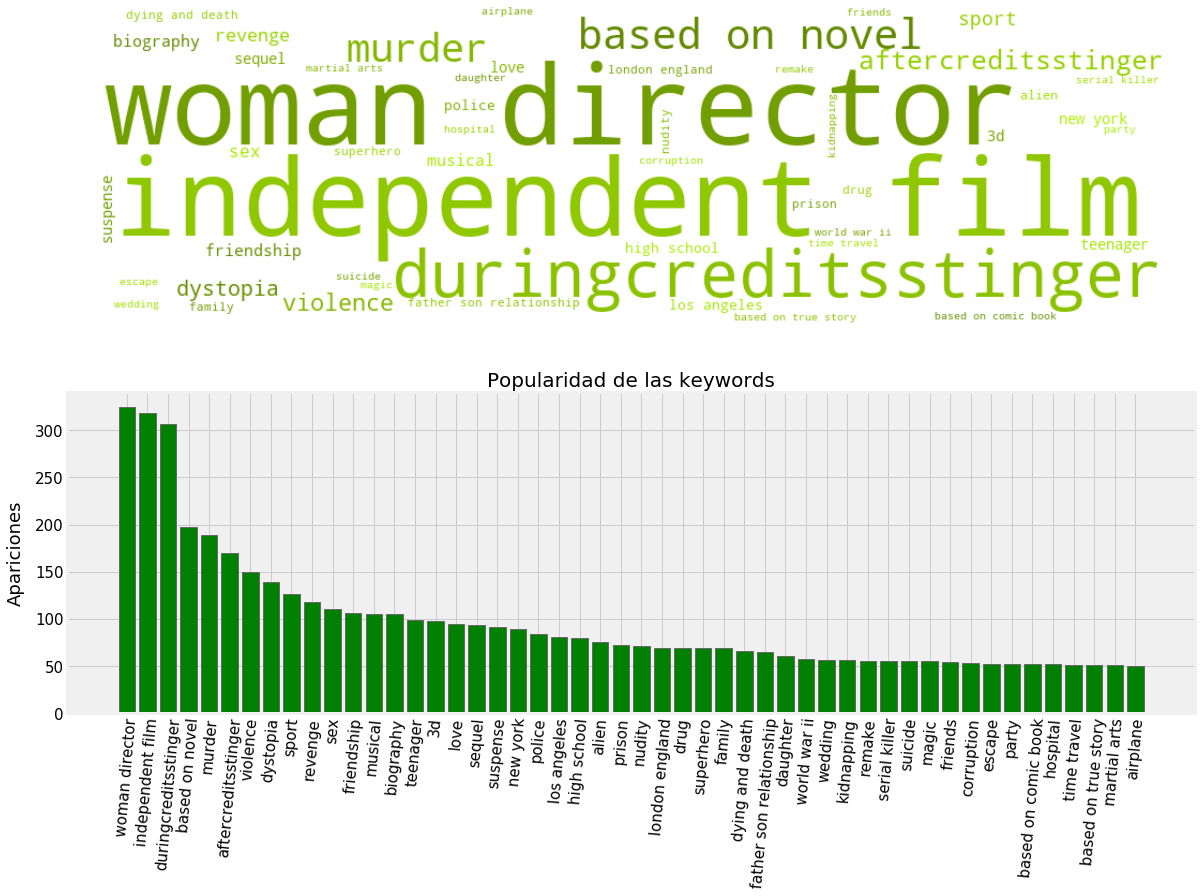
\includegraphics[width=10cm]{./contenido/imagenes/output_18_0.png}

\end{figure}
    { \hspace*{\fill} \\}
    
    \begin{center}\rule{0.5\linewidth}{\linethickness}\end{center}

\subsubsection{1.2 Factor de completitud: Valores
Faltantes}\label{factor-de-completitud-valores-faltantes}

El conjunto de datos consiste en 5043 películas o series que están
descritas mediante 28 variables. Como en todo análisis, habrá que trater
con los valores faltantes y, como un primer paso, se calcula la cantidad
de datos faltantes en cada variable:

    \begin{tcolorbox}[breakable, size=fbox, boxrule=1pt, pad at break*=1mm,colback=cellbackground, colframe=cellborder]
\prompt{In}{incolor}{13}{\hspace{4pt}}
\begin{Verbatim}[commandchars=\\\{\}]
\PY{n}{missing\PYZus{}df} \PY{o}{=} \PY{n}{df\PYZus{}initial}\PY{o}{.}\PY{n}{isnull}\PY{p}{(}\PY{p}{)}\PY{o}{.}\PY{n}{sum}\PY{p}{(}\PY{n}{axis}\PY{o}{=}\PY{l+m+mi}{0}\PY{p}{)}\PY{o}{.}\PY{n}{reset\PYZus{}index}\PY{p}{(}\PY{p}{)}
\PY{n}{missing\PYZus{}df}\PY{o}{.}\PY{n}{columns} \PY{o}{=} \PY{p}{[}\PY{l+s+s1}{\PYZsq{}}\PY{l+s+s1}{column\PYZus{}name}\PY{l+s+s1}{\PYZsq{}}\PY{p}{,} \PY{l+s+s1}{\PYZsq{}}\PY{l+s+s1}{missing\PYZus{}count}\PY{l+s+s1}{\PYZsq{}}\PY{p}{]}
\PY{n}{missing\PYZus{}df}\PY{p}{[}\PY{l+s+s1}{\PYZsq{}}\PY{l+s+s1}{filling\PYZus{}factor}\PY{l+s+s1}{\PYZsq{}}\PY{p}{]} \PY{o}{=} \PY{p}{(}\PY{n}{df\PYZus{}initial}\PY{o}{.}\PY{n}{shape}\PY{p}{[}\PY{l+m+mi}{0}\PY{p}{]} 
                                \PY{o}{\PYZhy{}} \PY{n}{missing\PYZus{}df}\PY{p}{[}\PY{l+s+s1}{\PYZsq{}}\PY{l+s+s1}{missing\PYZus{}count}\PY{l+s+s1}{\PYZsq{}}\PY{p}{]}\PY{p}{)} \PY{o}{/} \PY{n}{df\PYZus{}initial}\PY{o}{.}\PY{n}{shape}\PY{p}{[}\PY{l+m+mi}{0}\PY{p}{]} \PY{o}{*} \PY{l+m+mi}{100}
\PY{n}{missing\PYZus{}df}\PY{o}{.}\PY{n}{sort\PYZus{}values}\PY{p}{(}\PY{l+s+s1}{\PYZsq{}}\PY{l+s+s1}{filling\PYZus{}factor}\PY{l+s+s1}{\PYZsq{}}\PY{p}{)}\PY{o}{.}\PY{n}{reset\PYZus{}index}\PY{p}{(}\PY{n}{drop} \PY{o}{=} \PY{k+kc}{True}\PY{p}{)}
\end{Verbatim}
\end{tcolorbox}

            \begin{tcolorbox}[breakable, boxrule=.5pt, size=fbox, pad at break*=1mm, opacityfill=0]
\prompt{Out}{outcolor}{13}{\hspace{3.5pt}}
\begin{Verbatim}[commandchars=\\\{\}]
             column\_name  missing\_count  filling\_factor
0               homepage           3091       35.644389
1                tagline            844       82.427649
2                country            174       96.377264
3           actor\_3\_name             93       98.063710
4               language             86       98.209452
5           actor\_2\_name             63       98.688320
6           actor\_1\_name             53       98.896523
7          director\_name             30       99.375390
8               overview              3       99.937539
9               duration              2       99.958359
10            title\_year              1       99.979180
11          release\_date              1       99.979180
12       num\_voted\_users              0      100.000000
13          vote\_average              0      100.000000
14           movie\_title              0      100.000000
15                budget              0      100.000000
16      spoken\_languages              0      100.000000
17  production\_countries              0      100.000000
18  production\_companies              0      100.000000
19            popularity              0      100.000000
20        original\_title              0      100.000000
21         plot\_keywords              0      100.000000
22                    id              0      100.000000
23                genres              0      100.000000
24                status              0      100.000000
25                 gross              0      100.000000
\end{Verbatim}
\end{tcolorbox}
        
    Podemos ver que la integridad de los datos es bastante buena, ya que
únicamente 2 de las 28 variables tienen un factor de competitud menor
del 93\%.

    \begin{center}\rule{0.5\linewidth}{\linethickness}\end{center}

\subsubsection{1.3 Géneros}\label{guxe9neros}

    La variable \textbf{genres} será importante en la creación del sistema
de recomendación, dado que describe el contenido de la película. Para
ver exactamente qué generos son los mas populares, se usa la misma
aproximación que con las keywords.

    \begin{tcolorbox}[breakable, size=fbox, boxrule=1pt, pad at break*=1mm,colback=cellbackground, colframe=cellborder]
\prompt{In}{incolor}{14}{\hspace{4pt}}
\begin{Verbatim}[commandchars=\\\{\}]
\PY{n}{genre\PYZus{}labels} \PY{o}{=} \PY{n+nb}{set}\PY{p}{(}\PY{p}{)}
\PY{k}{for} \PY{n}{s} \PY{o+ow}{in} \PY{n}{df\PYZus{}initial}\PY{p}{[}\PY{l+s+s1}{\PYZsq{}}\PY{l+s+s1}{genres}\PY{l+s+s1}{\PYZsq{}}\PY{p}{]}\PY{o}{.}\PY{n}{str}\PY{o}{.}\PY{n}{split}\PY{p}{(}\PY{l+s+s1}{\PYZsq{}}\PY{l+s+s1}{|}\PY{l+s+s1}{\PYZsq{}}\PY{p}{)}\PY{o}{.}\PY{n}{values}\PY{p}{:}
    \PY{n}{genre\PYZus{}labels} \PY{o}{=} \PY{n}{genre\PYZus{}labels}\PY{o}{.}\PY{n}{union}\PY{p}{(}\PY{n+nb}{set}\PY{p}{(}\PY{n}{s}\PY{p}{)}\PY{p}{)}
\end{Verbatim}
\end{tcolorbox}

    y cada genero aparece las siguientes veces:

    \begin{tcolorbox}[breakable, size=fbox, boxrule=1pt, pad at break*=1mm,colback=cellbackground, colframe=cellborder]
\prompt{In}{incolor}{15}{\hspace{4pt}}
\begin{Verbatim}[commandchars=\\\{\}]
\PY{n}{keyword\PYZus{}occurences}\PY{p}{,} \PY{n}{dum} \PY{o}{=} \PY{n}{count\PYZus{}word}\PY{p}{(}\PY{n}{df\PYZus{}initial}\PY{p}{,} \PY{l+s+s1}{\PYZsq{}}\PY{l+s+s1}{genres}\PY{l+s+s1}{\PYZsq{}}\PY{p}{,} \PY{n}{genre\PYZus{}labels}\PY{p}{)}
\PY{n}{keyword\PYZus{}occurences}\PY{p}{[}\PY{p}{:}\PY{l+m+mi}{5}\PY{p}{]}
\end{Verbatim}
\end{tcolorbox}

            \begin{tcolorbox}[breakable, boxrule=.5pt, size=fbox, pad at break*=1mm, opacityfill=0]
\prompt{Out}{outcolor}{15}{\hspace{3.5pt}}
\begin{Verbatim}[commandchars=\\\{\}]
[['Drama', 2297],
 ['Comedy', 1722],
 ['Thriller', 1274],
 ['Action', 1154],
 ['Romance', 894]]
\end{Verbatim}
\end{tcolorbox}
        
    \begin{tcolorbox}[breakable, size=fbox, boxrule=1pt, pad at break*=1mm,colback=cellbackground, colframe=cellborder]
\prompt{In}{incolor}{16}{\hspace{4pt}}
\begin{Verbatim}[commandchars=\\\{\}]
\PY{n}{keyword\PYZus{}occurences} \PY{o}{=} \PY{p}{[}\PY{n}{x} \PY{k}{for} \PY{n}{x} \PY{o+ow}{in} \PY{n}{keyword\PYZus{}occurences} \PY{k}{if} \PY{n}{x}\PY{p}{[}\PY{l+m+mi}{0}\PY{p}{]}\PY{p}{]}
\end{Verbatim}
\end{tcolorbox}

    Se muestra el resultado como una nube de palabras

    \begin{tcolorbox}[breakable, size=fbox, boxrule=1pt, pad at break*=1mm,colback=cellbackground, colframe=cellborder]
\prompt{In}{incolor}{17}{\hspace{4pt}}
\begin{Verbatim}[commandchars=\\\{\}]
\PY{n}{words} \PY{o}{=} \PY{n+nb}{dict}\PY{p}{(}\PY{p}{)}
\PY{n}{trunc\PYZus{}occurences} \PY{o}{=} \PY{n}{keyword\PYZus{}occurences}\PY{p}{[}\PY{l+m+mi}{0}\PY{p}{:}\PY{l+m+mi}{50}\PY{p}{]}
\PY{k}{for} \PY{n}{s} \PY{o+ow}{in} \PY{n}{trunc\PYZus{}occurences}\PY{p}{:}
    \PY{n}{words}\PY{p}{[}\PY{n}{s}\PY{p}{[}\PY{l+m+mi}{0}\PY{p}{]}\PY{p}{]} \PY{o}{=} \PY{n}{s}\PY{p}{[}\PY{l+m+mi}{1}\PY{p}{]}
\PY{n}{tone} \PY{o}{=} \PY{l+m+mi}{100} \PY{c+c1}{\PYZsh{} define the color of the words}
\PY{n}{f}\PY{p}{,} \PY{n}{ax} \PY{o}{=} \PY{n}{plt}\PY{o}{.}\PY{n}{subplots}\PY{p}{(}\PY{n}{figsize}\PY{o}{=}\PY{p}{(}\PY{l+m+mi}{14}\PY{p}{,} \PY{l+m+mi}{6}\PY{p}{)}\PY{p}{)}
\PY{n}{wordcloud} \PY{o}{=} \PY{n}{WordCloud}\PY{p}{(}\PY{n}{width}\PY{o}{=}\PY{l+m+mi}{550}\PY{p}{,}\PY{n}{height}\PY{o}{=}\PY{l+m+mi}{300}\PY{p}{,} \PY{n}{background\PYZus{}color}\PY{o}{=}\PY{l+s+s1}{\PYZsq{}}\PY{l+s+s1}{white}\PY{l+s+s1}{\PYZsq{}}\PY{p}{,} 
                      \PY{n}{max\PYZus{}words}\PY{o}{=}\PY{l+m+mi}{1628}\PY{p}{,}\PY{n}{relative\PYZus{}scaling}\PY{o}{=}\PY{l+m+mf}{0.7}\PY{p}{,}
                      \PY{n}{color\PYZus{}func} \PY{o}{=} \PY{n}{random\PYZus{}color\PYZus{}func}\PY{p}{,}
                      \PY{n}{normalize\PYZus{}plurals}\PY{o}{=}\PY{k+kc}{False}\PY{p}{)}
\PY{n}{wordcloud}\PY{o}{.}\PY{n}{generate\PYZus{}from\PYZus{}frequencies}\PY{p}{(}\PY{n}{words}\PY{p}{)}
\PY{n}{plt}\PY{o}{.}\PY{n}{imshow}\PY{p}{(}\PY{n}{wordcloud}\PY{p}{,} \PY{n}{interpolation}\PY{o}{=}\PY{l+s+s2}{\PYZdq{}}\PY{l+s+s2}{bilinear}\PY{l+s+s2}{\PYZdq{}}\PY{p}{)}
\PY{n}{plt}\PY{o}{.}\PY{n}{axis}\PY{p}{(}\PY{l+s+s1}{\PYZsq{}}\PY{l+s+s1}{off}\PY{l+s+s1}{\PYZsq{}}\PY{p}{)}
\PY{n}{plt}\PY{o}{.}\PY{n}{show}\PY{p}{(}\PY{p}{)}
\end{Verbatim}
\end{tcolorbox}

\begin{figure}[h]
    \centering
    \captionsetup{width=10cm}
    
\includegraphics[width=10cm]{./contenido/imagenes/output_29_0.png}

\end{figure}
    { \hspace*{\fill} \\}
    
    \begin{center}\rule{0.5\linewidth}{\linethickness}\end{center}

\subsection{2. Limpieza}\label{limpieza}

\begin{center}\rule{0.5\linewidth}{\linethickness}\end{center}

\subsubsection{2.1 Entradas duplicadas}\label{entradas-duplicadas}

Hasta ahora, sólo mirabamos unas pocas variables e intentábamos
representar su contenido para tener una idea de su significado. Por
tanto, es ahora cuando empieza realmente la tarea de limpieza.

El primer paso consiste en buscar entradas duplicadas. Como un primer
paso, se comprueba si si las hay.

    \begin{tcolorbox}[breakable, size=fbox, boxrule=1pt, pad at break*=1mm,colback=cellbackground, colframe=cellborder]
\prompt{In}{incolor}{18}{\hspace{4pt}}
\begin{Verbatim}[commandchars=\\\{\}]
\PY{n}{doubled\PYZus{}entries} \PY{o}{=} \PY{n}{df\PYZus{}initial}\PY{p}{[}\PY{n}{df\PYZus{}initial}\PY{o}{.}\PY{n}{id}\PY{o}{.}\PY{n}{duplicated}\PY{p}{(}\PY{p}{)}\PY{p}{]}
\PY{n}{doubled\PYZus{}entries}\PY{o}{.}\PY{n}{shape}
\end{Verbatim}
\end{tcolorbox}

            \begin{tcolorbox}[breakable, boxrule=.5pt, size=fbox, pad at break*=1mm, opacityfill=0]
\prompt{Out}{outcolor}{18}{\hspace{3.5pt}}
\begin{Verbatim}[commandchars=\\\{\}]
(0, 26)
\end{Verbatim}
\end{tcolorbox}
        
    \begin{tcolorbox}[breakable, size=fbox, boxrule=1pt, pad at break*=1mm,colback=cellbackground, colframe=cellborder]
\prompt{In}{incolor}{19}{\hspace{4pt}}
\begin{Verbatim}[commandchars=\\\{\}]
\PY{n}{df\PYZus{}temp} \PY{o}{=} \PY{n}{df\PYZus{}initial}
\end{Verbatim}
\end{tcolorbox}

    Ahora examinamos lasfilas con entradas duplicadas teniendo en cuenta
únicamente las variables \textbf{movie\_title} y \textbf{title\_year},
and \textbf{director\_name}:

    \begin{tcolorbox}[breakable, size=fbox, boxrule=1pt, pad at break*=1mm,colback=cellbackground, colframe=cellborder]
\prompt{In}{incolor}{20}{\hspace{4pt}}
\begin{Verbatim}[commandchars=\\\{\}]
\PY{n}{list\PYZus{}var\PYZus{}duplicates} \PY{o}{=} \PY{p}{[}\PY{l+s+s1}{\PYZsq{}}\PY{l+s+s1}{movie\PYZus{}title}\PY{l+s+s1}{\PYZsq{}}\PY{p}{,} \PY{l+s+s1}{\PYZsq{}}\PY{l+s+s1}{title\PYZus{}year}\PY{l+s+s1}{\PYZsq{}}\PY{p}{,} \PY{l+s+s1}{\PYZsq{}}\PY{l+s+s1}{director\PYZus{}name}\PY{l+s+s1}{\PYZsq{}}\PY{p}{]}
\end{Verbatim}
\end{tcolorbox}

    Creamos una lista con las entradas con títulos idénticos:

    \begin{tcolorbox}[breakable, size=fbox, boxrule=1pt, pad at break*=1mm,colback=cellbackground, colframe=cellborder]
\prompt{In}{incolor}{21}{\hspace{4pt}}
\begin{Verbatim}[commandchars=\\\{\}]
\PY{n}{liste\PYZus{}duplicates} \PY{o}{=} \PY{n}{df\PYZus{}temp}\PY{p}{[}\PY{l+s+s1}{\PYZsq{}}\PY{l+s+s1}{movie\PYZus{}title}\PY{l+s+s1}{\PYZsq{}}\PY{p}{]}\PY{o}{.}\PY{n}{map}\PY{p}{(}\PY{n}{df\PYZus{}temp}\PY{p}{[}\PY{l+s+s1}{\PYZsq{}}\PY{l+s+s1}{movie\PYZus{}title}\PY{l+s+s1}{\PYZsq{}}\PY{p}{]}\PY{o}{.}\PY{n}{value\PYZus{}counts}\PY{p}{(}\PY{p}{)} \PY{o}{\PYZgt{}} \PY{l+m+mi}{1}\PY{p}{)}
\PY{n+nb}{print}\PY{p}{(}\PY{l+s+s2}{\PYZdq{}}\PY{l+s+s2}{Número de entradas duplicadas: }\PY{l+s+si}{\PYZob{}\PYZcb{}}\PY{l+s+s2}{\PYZdq{}}\PY{o}{.}\PY{n}{format}\PY{p}{(}
    \PY{n+nb}{len}\PY{p}{(}\PY{n}{df\PYZus{}temp}\PY{p}{[}\PY{n}{liste\PYZus{}duplicates}\PY{p}{]}\PY{p}{[}\PY{n}{list\PYZus{}var\PYZus{}duplicates}\PY{p}{]}\PY{p}{)}\PY{p}{)}\PY{p}{)}
\end{Verbatim}
\end{tcolorbox}

    \begin{Verbatim}[commandchars=\\\{\}]
Número de entradas duplicadas: 6
\end{Verbatim}

    y a continuación examinamos algunos casos. Dado que no hay demasiados
valores, es posible hacerlo a simple vista:

    \begin{tcolorbox}[breakable, size=fbox, boxrule=1pt, pad at break*=1mm,colback=cellbackground, colframe=cellborder]
\prompt{In}{incolor}{22}{\hspace{4pt}}
\begin{Verbatim}[commandchars=\\\{\}]
\PY{n}{df\PYZus{}temp}\PY{p}{[}\PY{n}{liste\PYZus{}duplicates}\PY{p}{]}\PY{p}{[}\PY{n}{list\PYZus{}var\PYZus{}duplicates}\PY{p}{]}\PY{o}{.}\PY{n}{sort\PYZus{}values}\PY{p}{(}\PY{l+s+s1}{\PYZsq{}}\PY{l+s+s1}{movie\PYZus{}title}\PY{l+s+s1}{\PYZsq{}}\PY{p}{)}
\end{Verbatim}
\end{tcolorbox}

            \begin{tcolorbox}[breakable, boxrule=.5pt, size=fbox, pad at break*=1mm, opacityfill=0]
\prompt{Out}{outcolor}{22}{\hspace{3.5pt}}
\begin{Verbatim}[commandchars=\\\{\}]
          movie\_title  title\_year        director\_name
1359           Batman      1989.0           Tim Burton
4267           Batman      1966.0  Leslie H. Martinson
3647  Out of the Blue      1980.0        Dennis Hopper
3693  Out of the Blue      2006.0       Robert Sarkies
972          The Host      2013.0        Andrew Niccol
2877         The Host      2006.0         Bong Joon-ho
\end{Verbatim}
\end{tcolorbox}
        
    Puede verse que estas películas son únicamente remakes.

    \begin{tcolorbox}[breakable, size=fbox, boxrule=1pt, pad at break*=1mm,colback=cellbackground, colframe=cellborder]
\prompt{In}{incolor}{ }{\hspace{4pt}}
\begin{Verbatim}[commandchars=\\\{\}]

\end{Verbatim}
\end{tcolorbox}

    \begin{tcolorbox}[breakable, size=fbox, boxrule=1pt, pad at break*=1mm,colback=cellbackground, colframe=cellborder]
\prompt{In}{incolor}{23}{\hspace{4pt}}
\begin{Verbatim}[commandchars=\\\{\}]
\PY{n}{df\PYZus{}duplicate\PYZus{}cleaned} \PY{o}{=} \PY{n}{df\PYZus{}temp}
\end{Verbatim}
\end{tcolorbox}

    \begin{center}\rule{0.5\linewidth}{\linethickness}\end{center}

\subsubsection{2.2 Limpieza de keywords}\label{limpieza-de-keywords}

Las keywords tendrán un papel fundamental en el funcionamiento del
sistema. De hecho, las recomendaciones se basaran en la similaridad
entre películas. Para medir esas similaridades, se mirarán las películas
descritas por las mismas keywords. Por tanto, el contenido de la
variable \textbf{plot\_keywords} debe ser analizado, ya que será muy
utilizado.

    \begin{center}\rule{0.5\linewidth}{\linethickness}\end{center}

\paragraph{2.2.1 Agrupamiento por lexema}\label{agrupamiento-por-lexema}

Cogemos las keywords que aparecen en \textbf{plot\_keywords}. Esta lista
se limpia usando NLTK. Finalmente, veremos la ocurrencia de cada
keyword.

    \begin{tcolorbox}[breakable, size=fbox, boxrule=1pt, pad at break*=1mm,colback=cellbackground, colframe=cellborder]
\prompt{In}{incolor}{24}{\hspace{4pt}}
\begin{Verbatim}[commandchars=\\\{\}]
\PY{k}{def} \PY{n+nf}{keywords\PYZus{}inventory}\PY{p}{(}\PY{n}{dataframe}\PY{p}{,} \PY{n}{column} \PY{o}{=} \PY{l+s+s1}{\PYZsq{}}\PY{l+s+s1}{plot\PYZus{}keywords}\PY{l+s+s1}{\PYZsq{}}\PY{p}{)}\PY{p}{:}
    \PY{l+s+sd}{\PYZdq{}\PYZdq{}\PYZdq{}Devuelve un diccionario con las palabras que derivan de cada lexema}
\PY{l+s+sd}{    a partir de un DataFrame y la columna de la que se quiere extraer}
\PY{l+s+sd}{    }
\PY{l+s+sd}{    Args:}
\PY{l+s+sd}{        dataframe (pd.DataFrame): DataFrame del que obtener la información.}
\PY{l+s+sd}{        column (str, optional): Nombre de la columna. Defaults to \PYZsq{}plot\PYZus{}keywords\PYZsq{}.}
\PY{l+s+sd}{    }
\PY{l+s+sd}{    Returns:}
\PY{l+s+sd}{        list: Keywords finales que aparecen}
\PY{l+s+sd}{        dict: Relación lexema \PYZlt{}\PYZhy{}\PYZgt{} palabras}
\PY{l+s+sd}{        dict: Palabra más corta derivada del lexema}
\PY{l+s+sd}{    \PYZdq{}\PYZdq{}\PYZdq{}}
    \PY{n}{PS} \PY{o}{=} \PY{n}{nltk}\PY{o}{.}\PY{n}{stem}\PY{o}{.}\PY{n}{PorterStemmer}\PY{p}{(}\PY{p}{)}
    \PY{n}{keywords\PYZus{}roots}  \PY{o}{=} \PY{n+nb}{dict}\PY{p}{(}\PY{p}{)}  \PY{c+c1}{\PYZsh{} recoger las palabras de cada lexema}
    \PY{n}{keywords\PYZus{}select} \PY{o}{=} \PY{n+nb}{dict}\PY{p}{(}\PY{p}{)}  \PY{c+c1}{\PYZsh{} asociacion: lexema \PYZlt{}\PYZhy{}\PYZgt{} keyword}
    \PY{n}{category\PYZus{}keys} \PY{o}{=} \PY{p}{[}\PY{p}{]}
    \PY{n}{icount} \PY{o}{=} \PY{l+m+mi}{0}
    \PY{k}{for} \PY{n}{s} \PY{o+ow}{in} \PY{n}{dataframe}\PY{p}{[}\PY{n}{column}\PY{p}{]}\PY{p}{:}
        \PY{k}{if} \PY{n}{pd}\PY{o}{.}\PY{n}{isnull}\PY{p}{(}\PY{n}{s}\PY{p}{)}\PY{p}{:} \PY{k}{continue}
        \PY{k}{for} \PY{n}{t} \PY{o+ow}{in} \PY{n}{s}\PY{o}{.}\PY{n}{split}\PY{p}{(}\PY{l+s+s1}{\PYZsq{}}\PY{l+s+s1}{|}\PY{l+s+s1}{\PYZsq{}}\PY{p}{)}\PY{p}{:}
            \PY{n}{t} \PY{o}{=} \PY{n}{t}\PY{o}{.}\PY{n}{lower}\PY{p}{(}\PY{p}{)} \PY{p}{;} \PY{n}{root} \PY{o}{=} \PY{n}{PS}\PY{o}{.}\PY{n}{stem}\PY{p}{(}\PY{n}{t}\PY{p}{)}
            \PY{c+c1}{\PYZsh{} Para cada lexema, un set con las palabras que lo usan}
            \PY{k}{if} \PY{n}{root} \PY{o+ow}{in} \PY{n}{keywords\PYZus{}roots}\PY{p}{:}                
                \PY{n}{keywords\PYZus{}roots}\PY{p}{[}\PY{n}{root}\PY{p}{]}\PY{o}{.}\PY{n}{add}\PY{p}{(}\PY{n}{t}\PY{p}{)}
            \PY{k}{else}\PY{p}{:}
                \PY{n}{keywords\PYZus{}roots}\PY{p}{[}\PY{n}{root}\PY{p}{]} \PY{o}{=} \PY{p}{\PYZob{}}\PY{n}{t}\PY{p}{\PYZcb{}}
    
    \PY{k}{for} \PY{n}{s} \PY{o+ow}{in} \PY{n}{keywords\PYZus{}roots}\PY{o}{.}\PY{n}{keys}\PY{p}{(}\PY{p}{)}\PY{p}{:}
        \PY{k}{if} \PY{n+nb}{len}\PY{p}{(}\PY{n}{keywords\PYZus{}roots}\PY{p}{[}\PY{n}{s}\PY{p}{]}\PY{p}{)} \PY{o}{\PYZgt{}} \PY{l+m+mi}{1}\PY{p}{:}  
            \PY{n}{min\PYZus{}length} \PY{o}{=} \PY{l+m+mi}{1000}
            \PY{k}{for} \PY{n}{k} \PY{o+ow}{in} \PY{n}{keywords\PYZus{}roots}\PY{p}{[}\PY{n}{s}\PY{p}{]}\PY{p}{:}
                \PY{k}{if} \PY{n+nb}{len}\PY{p}{(}\PY{n}{k}\PY{p}{)} \PY{o}{\PYZlt{}} \PY{n}{min\PYZus{}length}\PY{p}{:}
                    \PY{n}{key} \PY{o}{=} \PY{n}{k} \PY{p}{;} \PY{n}{min\PYZus{}length} \PY{o}{=} \PY{n+nb}{len}\PY{p}{(}\PY{n}{k}\PY{p}{)}            
            \PY{n}{category\PYZus{}keys}\PY{o}{.}\PY{n}{append}\PY{p}{(}\PY{n}{key}\PY{p}{)}
            \PY{n}{keywords\PYZus{}select}\PY{p}{[}\PY{n}{s}\PY{p}{]} \PY{o}{=} \PY{n}{key}
        \PY{k}{else}\PY{p}{:}
            \PY{n}{category\PYZus{}keys}\PY{o}{.}\PY{n}{append}\PY{p}{(}\PY{n+nb}{list}\PY{p}{(}\PY{n}{keywords\PYZus{}roots}\PY{p}{[}\PY{n}{s}\PY{p}{]}\PY{p}{)}\PY{p}{[}\PY{l+m+mi}{0}\PY{p}{]}\PY{p}{)}
            \PY{n}{keywords\PYZus{}select}\PY{p}{[}\PY{n}{s}\PY{p}{]} \PY{o}{=} \PY{n+nb}{list}\PY{p}{(}\PY{n}{keywords\PYZus{}roots}\PY{p}{[}\PY{n}{s}\PY{p}{]}\PY{p}{)}\PY{p}{[}\PY{l+m+mi}{0}\PY{p}{]}
                   
    \PY{n+nb}{print}\PY{p}{(}\PY{l+s+s2}{\PYZdq{}}\PY{l+s+s2}{Número de keywords en la variable: }\PY{l+s+s2}{\PYZsq{}}\PY{l+s+si}{\PYZob{}\PYZcb{}}\PY{l+s+s2}{\PYZsq{}}\PY{l+s+s2}{: }\PY{l+s+si}{\PYZob{}\PYZcb{}}\PY{l+s+s2}{\PYZdq{}}\PY{o}{.}\PY{n}{format}\PY{p}{(}\PY{n}{column}\PY{p}{,}\PY{n+nb}{len}\PY{p}{(}\PY{n}{category\PYZus{}keys}\PY{p}{)}\PY{p}{)}\PY{p}{)}
    \PY{k}{return} \PY{n}{category\PYZus{}keys}\PY{p}{,} \PY{n}{keywords\PYZus{}roots}\PY{p}{,} \PY{n}{keywords\PYZus{}select}
\end{Verbatim}
\end{tcolorbox}

    \begin{tcolorbox}[breakable, size=fbox, boxrule=1pt, pad at break*=1mm,colback=cellbackground, colframe=cellborder]
\prompt{In}{incolor}{25}{\hspace{4pt}}
\begin{Verbatim}[commandchars=\\\{\}]
\PY{n}{keywords}\PY{p}{,} \PY{n}{keywords\PYZus{}roots}\PY{p}{,} \PY{n}{keywords\PYZus{}select} \PY{o}{=} \PY{n}{keywords\PYZus{}inventory}\PY{p}{(}\PY{n}{df\PYZus{}duplicate\PYZus{}cleaned}\PY{p}{,}
                                                               \PY{n}{column} \PY{o}{=} \PY{l+s+s1}{\PYZsq{}}\PY{l+s+s1}{plot\PYZus{}keywords}\PY{l+s+s1}{\PYZsq{}}\PY{p}{)}
\end{Verbatim}
\end{tcolorbox}

    \begin{Verbatim}[commandchars=\\\{\}]
Número de keywords en la variable: 'plot\_keywords': 9474
\end{Verbatim}

    \begin{tcolorbox}[breakable, size=fbox, boxrule=1pt, pad at break*=1mm,colback=cellbackground, colframe=cellborder]
\prompt{In}{incolor}{26}{\hspace{4pt}}
\begin{Verbatim}[commandchars=\\\{\}]
\PY{c+c1}{\PYZsh{} Muestra de keywords que aparecen en formas similares}
\PY{c+c1}{\PYZsh{}\PYZhy{}\PYZhy{}\PYZhy{}\PYZhy{}\PYZhy{}\PYZhy{}\PYZhy{}\PYZhy{}\PYZhy{}\PYZhy{}\PYZhy{}\PYZhy{}\PYZhy{}\PYZhy{}\PYZhy{}\PYZhy{}\PYZhy{}\PYZhy{}\PYZhy{}\PYZhy{}\PYZhy{}\PYZhy{}\PYZhy{}\PYZhy{}\PYZhy{}\PYZhy{}\PYZhy{}\PYZhy{}\PYZhy{}\PYZhy{}\PYZhy{}\PYZhy{}\PYZhy{}\PYZhy{}\PYZhy{}\PYZhy{}\PYZhy{}\PYZhy{}\PYZhy{}\PYZhy{}\PYZhy{}\PYZhy{}\PYZhy{}\PYZhy{}\PYZhy{}\PYZhy{}\PYZhy{}\PYZhy{}\PYZhy{}\PYZhy{}\PYZhy{}\PYZhy{}\PYZhy{}\PYZhy{}\PYZhy{}\PYZhy{}\PYZhy{}\PYZhy{}\PYZhy{}\PYZhy{}}
\PY{n}{icount} \PY{o}{=} \PY{l+m+mi}{0}
\PY{k}{for} \PY{n}{s} \PY{o+ow}{in} \PY{n}{keywords\PYZus{}roots}\PY{o}{.}\PY{n}{keys}\PY{p}{(}\PY{p}{)}\PY{p}{:}
    \PY{k}{if} \PY{n+nb}{len}\PY{p}{(}\PY{n}{keywords\PYZus{}roots}\PY{p}{[}\PY{n}{s}\PY{p}{]}\PY{p}{)} \PY{o}{\PYZgt{}} \PY{l+m+mi}{1}\PY{p}{:} 
        \PY{n}{icount} \PY{o}{+}\PY{o}{=} \PY{l+m+mi}{1}
        \PY{k}{if} \PY{n}{icount} \PY{o}{\PYZlt{}} \PY{l+m+mi}{15}\PY{p}{:} \PY{n+nb}{print}\PY{p}{(}\PY{n}{icount}\PY{p}{,} \PY{n}{keywords\PYZus{}roots}\PY{p}{[}\PY{n}{s}\PY{p}{]}\PY{p}{,} \PY{n+nb}{len}\PY{p}{(}\PY{n}{keywords\PYZus{}roots}\PY{p}{[}\PY{n}{s}\PY{p}{]}\PY{p}{)}\PY{p}{)}
\end{Verbatim}
\end{tcolorbox}

    \begin{Verbatim}[commandchars=\\\{\}]
1 \{'alien', 'alienation'\} 2
2 \{'spying', 'spy'\} 2
3 \{'vigilante', 'vigilantism'\} 2
4 \{'terror', 'terrorism'\} 2
5 \{'flooding', 'flood'\} 2
6 \{'spiders', 'spider'\} 2
7 \{'horses', 'horse'\} 2
8 \{'musical', 'music'\} 2
9 \{'anime', 'animation', 'animal'\} 3
10 \{'compass', 'compassion'\} 2
11 \{'train', 'training'\} 2
12 \{'sailing', 'sail'\} 2
13 \{'time travel', 'time traveler'\} 2
14 \{'orcs', 'orc'\} 2
\end{Verbatim}

    \begin{tcolorbox}[breakable, size=fbox, boxrule=1pt, pad at break*=1mm,colback=cellbackground, colframe=cellborder]
\prompt{In}{incolor}{27}{\hspace{4pt}}
\begin{Verbatim}[commandchars=\\\{\}]
\PY{c+c1}{\PYZsh{} Reemplazo de keywords por su forma principal}
\PY{c+c1}{\PYZsh{}\PYZhy{}\PYZhy{}\PYZhy{}\PYZhy{}\PYZhy{}\PYZhy{}\PYZhy{}\PYZhy{}\PYZhy{}\PYZhy{}\PYZhy{}\PYZhy{}\PYZhy{}\PYZhy{}\PYZhy{}\PYZhy{}\PYZhy{}\PYZhy{}\PYZhy{}\PYZhy{}\PYZhy{}\PYZhy{}\PYZhy{}\PYZhy{}\PYZhy{}\PYZhy{}\PYZhy{}\PYZhy{}\PYZhy{}\PYZhy{}\PYZhy{}\PYZhy{}\PYZhy{}\PYZhy{}\PYZhy{}\PYZhy{}\PYZhy{}\PYZhy{}\PYZhy{}\PYZhy{}\PYZhy{}\PYZhy{}\PYZhy{}\PYZhy{}\PYZhy{}\PYZhy{}}
\PY{k}{def} \PY{n+nf}{df\PYZus{}keywords\PYZus{}replacement}\PY{p}{(}\PY{n}{df}\PY{p}{,} \PY{n}{replacement\PYZus{}dict}\PY{p}{,} \PY{n}{roots} \PY{o}{=} \PY{k+kc}{False}\PY{p}{,} \PY{n}{column} \PY{o}{=} \PY{l+s+s1}{\PYZsq{}}\PY{l+s+s1}{plot\PYZus{}keywords}\PY{l+s+s1}{\PYZsq{}}\PY{p}{)}\PY{p}{:}
    \PY{l+s+sd}{\PYZdq{}\PYZdq{}\PYZdq{}Reemplaza las palabras clave de una película por las formas básicas de las mismas.}

\PY{l+s+sd}{    Args:}
\PY{l+s+sd}{        df (pd.DataFrame): DataFrame que contiene la información de las películas}
\PY{l+s+sd}{        replacement\PYZus{}dict (dict): Diccionario con los cambios}
\PY{l+s+sd}{        roots (bool, optional): Controla si se obtienen las raices de las palabras de las}
\PY{l+s+sd}{        keywords. Defaults to False.}
\PY{l+s+sd}{        column (str, optional): Columna en la que realizar la transformación. Defaults to \PYZsq{}plot\PYZus{}keywords\PYZsq{}.}

\PY{l+s+sd}{    Returns:}
\PY{l+s+sd}{        pd.DataFrame: DataFrame con las sustituciones realizadas}
\PY{l+s+sd}{    \PYZdq{}\PYZdq{}\PYZdq{}}
    \PY{n}{PS} \PY{o}{=} \PY{n}{nltk}\PY{o}{.}\PY{n}{stem}\PY{o}{.}\PY{n}{PorterStemmer}\PY{p}{(}\PY{p}{)}
    \PY{n}{df\PYZus{}new} \PY{o}{=} \PY{n}{df}\PY{o}{.}\PY{n}{copy}\PY{p}{(}\PY{n}{deep} \PY{o}{=} \PY{k+kc}{True}\PY{p}{)}
    \PY{k}{for} \PY{n}{index}\PY{p}{,} \PY{n}{row} \PY{o+ow}{in} \PY{n}{df\PYZus{}new}\PY{o}{.}\PY{n}{iterrows}\PY{p}{(}\PY{p}{)}\PY{p}{:}
        \PY{n}{chain} \PY{o}{=} \PY{n}{row}\PY{p}{[}\PY{n}{column}\PY{p}{]}
        \PY{k}{if} \PY{n}{pd}\PY{o}{.}\PY{n}{isnull}\PY{p}{(}\PY{n}{chain}\PY{p}{)}\PY{p}{:} \PY{k}{continue}
        \PY{n}{new\PYZus{}list} \PY{o}{=} \PY{p}{[}\PY{p}{]}
        \PY{k}{for} \PY{n}{s} \PY{o+ow}{in} \PY{n}{chain}\PY{o}{.}\PY{n}{split}\PY{p}{(}\PY{l+s+s1}{\PYZsq{}}\PY{l+s+s1}{|}\PY{l+s+s1}{\PYZsq{}}\PY{p}{)}\PY{p}{:} 
            \PY{n}{key} \PY{o}{=} \PY{n}{PS}\PY{o}{.}\PY{n}{stem}\PY{p}{(}\PY{n}{s}\PY{p}{)} \PY{k}{if} \PY{n}{roots} \PY{k}{else} \PY{n}{s}
            \PY{k}{if} \PY{n}{key} \PY{o+ow}{in} \PY{n}{replacement\PYZus{}dict}\PY{o}{.}\PY{n}{keys}\PY{p}{(}\PY{p}{)}\PY{p}{:}
                \PY{n}{new\PYZus{}list}\PY{o}{.}\PY{n}{append}\PY{p}{(}\PY{n}{replacement\PYZus{}dict}\PY{p}{[}\PY{n}{key}\PY{p}{]}\PY{p}{)}
            \PY{k}{else}\PY{p}{:}
                \PY{n}{new\PYZus{}list}\PY{o}{.}\PY{n}{append}\PY{p}{(}\PY{n}{s}\PY{p}{)}       
        \PY{n}{df\PYZus{}new}\PY{o}{.}\PY{n}{set\PYZus{}value}\PY{p}{(}\PY{n}{index}\PY{p}{,} \PY{n}{column}\PY{p}{,} \PY{l+s+s1}{\PYZsq{}}\PY{l+s+s1}{|}\PY{l+s+s1}{\PYZsq{}}\PY{o}{.}\PY{n}{join}\PY{p}{(}\PY{n}{new\PYZus{}list}\PY{p}{)}\PY{p}{)} 
    \PY{k}{return} \PY{n}{df\PYZus{}new}
\end{Verbatim}
\end{tcolorbox}

    \begin{tcolorbox}[breakable, size=fbox, boxrule=1pt, pad at break*=1mm,colback=cellbackground, colframe=cellborder]
\prompt{In}{incolor}{28}{\hspace{4pt}}
\begin{Verbatim}[commandchars=\\\{\}]
\PY{c+c1}{\PYZsh{} Reemplazo de keywords por su forma principal}
\PY{c+c1}{\PYZsh{}\PYZhy{}\PYZhy{}\PYZhy{}\PYZhy{}\PYZhy{}\PYZhy{}\PYZhy{}\PYZhy{}\PYZhy{}\PYZhy{}\PYZhy{}\PYZhy{}\PYZhy{}\PYZhy{}\PYZhy{}\PYZhy{}\PYZhy{}\PYZhy{}\PYZhy{}\PYZhy{}\PYZhy{}\PYZhy{}\PYZhy{}\PYZhy{}\PYZhy{}\PYZhy{}\PYZhy{}\PYZhy{}\PYZhy{}\PYZhy{}\PYZhy{}\PYZhy{}\PYZhy{}\PYZhy{}\PYZhy{}\PYZhy{}\PYZhy{}\PYZhy{}\PYZhy{}\PYZhy{}\PYZhy{}\PYZhy{}\PYZhy{}\PYZhy{}\PYZhy{}\PYZhy{}\PYZhy{}\PYZhy{}\PYZhy{}}
\PY{n}{df\PYZus{}keywords\PYZus{}cleaned} \PY{o}{=} \PY{n}{df\PYZus{}keywords\PYZus{}replacement}\PY{p}{(}\PY{n}{df\PYZus{}duplicate\PYZus{}cleaned}\PY{p}{,} \PY{n}{keywords\PYZus{}select}\PY{p}{,}
                                               \PY{n}{roots} \PY{o}{=} \PY{k+kc}{True}\PY{p}{)}
\end{Verbatim}
\end{tcolorbox}

    \begin{tcolorbox}[breakable, size=fbox, boxrule=1pt, pad at break*=1mm,colback=cellbackground, colframe=cellborder]
\prompt{In}{incolor}{29}{\hspace{4pt}}
\begin{Verbatim}[commandchars=\\\{\}]
\PY{c+c1}{\PYZsh{} Conteo de la repetición de cada Keyword}
\PY{c+c1}{\PYZsh{}\PYZhy{}\PYZhy{}\PYZhy{}\PYZhy{}\PYZhy{}\PYZhy{}\PYZhy{}\PYZhy{}\PYZhy{}\PYZhy{}\PYZhy{}\PYZhy{}\PYZhy{}\PYZhy{}\PYZhy{}\PYZhy{}\PYZhy{}\PYZhy{}\PYZhy{}\PYZhy{}\PYZhy{}\PYZhy{}\PYZhy{}\PYZhy{}\PYZhy{}\PYZhy{}\PYZhy{}\PYZhy{}\PYZhy{}\PYZhy{}\PYZhy{}\PYZhy{}\PYZhy{}\PYZhy{}}
\PY{n}{keyword\PYZus{}occurences}\PY{p}{,} \PY{n}{keywords\PYZus{}count} \PY{o}{=} \PY{n}{count\PYZus{}word}\PY{p}{(}\PY{n}{df\PYZus{}keywords\PYZus{}cleaned}\PY{p}{,}\PY{l+s+s1}{\PYZsq{}}\PY{l+s+s1}{plot\PYZus{}keywords}\PY{l+s+s1}{\PYZsq{}}\PY{p}{,}\PY{n}{keywords}\PY{p}{)}
\PY{n}{keyword\PYZus{}occurences}\PY{p}{[}\PY{p}{:}\PY{l+m+mi}{5}\PY{p}{]}
\end{Verbatim}
\end{tcolorbox}

            \begin{tcolorbox}[breakable, boxrule=.5pt, size=fbox, pad at break*=1mm, opacityfill=0]
\prompt{Out}{outcolor}{29}{\hspace{3.5pt}}
\begin{Verbatim}[commandchars=\\\{\}]
[['', 412],
 ['woman director', 324],
 ['independent film', 318],
 ['duringcreditsstinger', 307],
 ['based on novel', 197]]
\end{Verbatim}
\end{tcolorbox}
        
    \begin{tcolorbox}[breakable, size=fbox, boxrule=1pt, pad at break*=1mm,colback=cellbackground, colframe=cellborder]
\prompt{In}{incolor}{30}{\hspace{4pt}}
\begin{Verbatim}[commandchars=\\\{\}]
\PY{n+nb}{len}\PY{p}{(}\PY{n}{keywords\PYZus{}count}\PY{p}{)}
\end{Verbatim}
\end{tcolorbox}

            \begin{tcolorbox}[breakable, boxrule=.5pt, size=fbox, pad at break*=1mm, opacityfill=0]
\prompt{Out}{outcolor}{30}{\hspace{3.5pt}}
\begin{Verbatim}[commandchars=\\\{\}]
9474
\end{Verbatim}
\end{tcolorbox}
        
    \begin{center}\rule{0.5\linewidth}{\linethickness}\end{center}

\paragraph{\texorpdfstring{2.2.2 Grupos de
\emph{sinónimos}}{2.2.2 Grupos de sinónimos}}\label{grupos-de-sinuxf3nimos}

Limpiamos la lista de keywords en dos pasos. En un primer paso, se
suprimer las keywords que aparecen menos de 5 veces y se reemplazan por
un sinónimo de mayor frecuencia. En un segundo paso, se suprimen las
keywords que aparecen en menos de 3 películas.

    \begin{tcolorbox}[breakable, size=fbox, boxrule=1pt, pad at break*=1mm,colback=cellbackground, colframe=cellborder]
\prompt{In}{incolor}{31}{\hspace{4pt}}
\begin{Verbatim}[commandchars=\\\{\}]
\PY{c+c1}{\PYZsh{} Obtener los sinónimos de la palabra \PYZsq{}keyword\PYZsq{}}
\PY{c+c1}{\PYZsh{}\PYZhy{}\PYZhy{}\PYZhy{}\PYZhy{}\PYZhy{}\PYZhy{}\PYZhy{}\PYZhy{}\PYZhy{}\PYZhy{}\PYZhy{}\PYZhy{}\PYZhy{}\PYZhy{}\PYZhy{}\PYZhy{}\PYZhy{}\PYZhy{}\PYZhy{}\PYZhy{}\PYZhy{}\PYZhy{}\PYZhy{}\PYZhy{}\PYZhy{}\PYZhy{}\PYZhy{}\PYZhy{}\PYZhy{}\PYZhy{}\PYZhy{}\PYZhy{}\PYZhy{}\PYZhy{}\PYZhy{}\PYZhy{}\PYZhy{}\PYZhy{}\PYZhy{}\PYZhy{}\PYZhy{}\PYZhy{}\PYZhy{}\PYZhy{}\PYZhy{}\PYZhy{}\PYZhy{}\PYZhy{}\PYZhy{}\PYZhy{}\PYZhy{}\PYZhy{}\PYZhy{}\PYZhy{}\PYZhy{}\PYZhy{}\PYZhy{}\PYZhy{}\PYZhy{}\PYZhy{}\PYZhy{}\PYZhy{}}
\PY{k}{def} \PY{n+nf}{get\PYZus{}synonyms}\PY{p}{(}\PY{n}{keyword}\PY{p}{)}\PY{p}{:}
    \PY{l+s+sd}{\PYZdq{}\PYZdq{}\PYZdq{}Se obtienen los sinónimos sustantivos de una palabra}
\PY{l+s+sd}{    }
\PY{l+s+sd}{    Args:}
\PY{l+s+sd}{        keyword (str): Palabra de la que obtener los sinónimos}
\PY{l+s+sd}{    }
\PY{l+s+sd}{    Returns:}
\PY{l+s+sd}{        list: Lista con los sinónimos}
\PY{l+s+sd}{    \PYZdq{}\PYZdq{}\PYZdq{}}

    \PY{n}{lemma} \PY{o}{=} \PY{n+nb}{set}\PY{p}{(}\PY{p}{)}
    \PY{k}{for} \PY{n}{ss} \PY{o+ow}{in} \PY{n}{wordnet}\PY{o}{.}\PY{n}{synsets}\PY{p}{(}\PY{n}{keyword}\PY{p}{)}\PY{p}{:}
        \PY{k}{for} \PY{n}{w} \PY{o+ow}{in} \PY{n}{ss}\PY{o}{.}\PY{n}{lemma\PYZus{}names}\PY{p}{(}\PY{p}{)}\PY{p}{:}
            \PY{c+c1}{\PYZsh{}\PYZus{}\PYZus{}\PYZus{}\PYZus{}\PYZus{}\PYZus{}\PYZus{}\PYZus{}\PYZus{}\PYZus{}\PYZus{}\PYZus{}\PYZus{}\PYZus{}\PYZus{}\PYZus{}\PYZus{}\PYZus{}\PYZus{}\PYZus{}\PYZus{}\PYZus{}\PYZus{}\PYZus{}\PYZus{}\PYZus{}\PYZus{}\PYZus{}\PYZus{}\PYZus{}\PYZus{}}
            \PY{c+c1}{\PYZsh{}  Obtenemos los sinónimos que son sustantivos}
            \PY{n}{index} \PY{o}{=} \PY{n}{ss}\PY{o}{.}\PY{n}{name}\PY{p}{(}\PY{p}{)}\PY{o}{.}\PY{n}{find}\PY{p}{(}\PY{l+s+s1}{\PYZsq{}}\PY{l+s+s1}{.}\PY{l+s+s1}{\PYZsq{}}\PY{p}{)}\PY{o}{+}\PY{l+m+mi}{1}
            \PY{k}{if} \PY{n}{ss}\PY{o}{.}\PY{n}{name}\PY{p}{(}\PY{p}{)}\PY{p}{[}\PY{n}{index}\PY{p}{]} \PY{o}{==} \PY{l+s+s1}{\PYZsq{}}\PY{l+s+s1}{n}\PY{l+s+s1}{\PYZsq{}}\PY{p}{:} \PY{n}{lemma}\PY{o}{.}\PY{n}{add}\PY{p}{(}\PY{n}{w}\PY{o}{.}\PY{n}{lower}\PY{p}{(}\PY{p}{)}\PY{o}{.}\PY{n}{replace}\PY{p}{(}\PY{l+s+s1}{\PYZsq{}}\PY{l+s+s1}{\PYZus{}}\PY{l+s+s1}{\PYZsq{}}\PY{p}{,}\PY{l+s+s1}{\PYZsq{}}\PY{l+s+s1}{ }\PY{l+s+s1}{\PYZsq{}}\PY{p}{)}\PY{p}{)}
    \PY{k}{return} \PY{n}{lemma}   
\end{Verbatim}
\end{tcolorbox}

    \begin{tcolorbox}[breakable, size=fbox, boxrule=1pt, pad at break*=1mm,colback=cellbackground, colframe=cellborder]
\prompt{In}{incolor}{32}{\hspace{4pt}}
\begin{Verbatim}[commandchars=\\\{\}]
\PY{c+c1}{\PYZsh{} Ejemplo de una lista de sinónimos dados por NLTK}
\PY{c+c1}{\PYZsh{}\PYZhy{}\PYZhy{}\PYZhy{}\PYZhy{}\PYZhy{}\PYZhy{}\PYZhy{}\PYZhy{}\PYZhy{}\PYZhy{}\PYZhy{}\PYZhy{}\PYZhy{}\PYZhy{}\PYZhy{}\PYZhy{}\PYZhy{}\PYZhy{}\PYZhy{}\PYZhy{}\PYZhy{}\PYZhy{}\PYZhy{}\PYZhy{}\PYZhy{}\PYZhy{}\PYZhy{}\PYZhy{}\PYZhy{}\PYZhy{}\PYZhy{}\PYZhy{}\PYZhy{}\PYZhy{}\PYZhy{}\PYZhy{}\PYZhy{}\PYZhy{}\PYZhy{}\PYZhy{}\PYZhy{}\PYZhy{}\PYZhy{}\PYZhy{}\PYZhy{}\PYZhy{}\PYZhy{}\PYZhy{}\PYZhy{}\PYZhy{}\PYZhy{}}
\PY{n}{keyword} \PY{o}{=} \PY{l+s+s1}{\PYZsq{}}\PY{l+s+s1}{alien}\PY{l+s+s1}{\PYZsq{}}
\PY{n}{lemma} \PY{o}{=} \PY{n}{get\PYZus{}synonyms}\PY{p}{(}\PY{n}{keyword}\PY{p}{)}
\PY{k}{for} \PY{n}{s} \PY{o+ow}{in} \PY{n}{lemma}\PY{p}{:}
    \PY{n+nb}{print}\PY{p}{(}\PY{l+s+s1}{\PYZsq{}}\PY{l+s+s1}{ }\PY{l+s+s1}{\PYZdq{}}\PY{l+s+si}{\PYZob{}:\PYZlt{}30\PYZcb{}}\PY{l+s+s1}{\PYZdq{}}\PY{l+s+s1}{ in keywords list \PYZhy{}\PYZgt{} }\PY{l+s+si}{\PYZob{}\PYZcb{}}\PY{l+s+s1}{ }\PY{l+s+si}{\PYZob{}\PYZcb{}}\PY{l+s+s1}{\PYZsq{}}\PY{o}{.}\PY{n}{format}\PY{p}{(}\PY{n}{s}\PY{p}{,} \PY{n}{s} \PY{o+ow}{in} \PY{n}{keywords}\PY{p}{,}
                                                \PY{n}{keywords\PYZus{}count}\PY{p}{[}\PY{n}{s}\PY{p}{]} \PY{k}{if} \PY{n}{s} \PY{o+ow}{in} \PY{n}{keywords} \PY{k}{else} \PY{l+m+mi}{0} \PY{p}{)}\PY{p}{)}
\end{Verbatim}
\end{tcolorbox}

    \begin{Verbatim}[commandchars=\\\{\}]
 "unknown                       " in keywords list -> False 0
 "foreigner                     " in keywords list -> False 0
 "noncitizen                    " in keywords list -> False 0
 "extraterrestrial being        " in keywords list -> False 0
 "stranger                      " in keywords list -> True 7
 "alien                         " in keywords list -> True 80
 "extraterrestrial              " in keywords list -> True 4
 "outlander                     " in keywords list -> False 0
\end{Verbatim}

    \begin{tcolorbox}[breakable, size=fbox, boxrule=1pt, pad at break*=1mm,colback=cellbackground, colframe=cellborder]
\prompt{In}{incolor}{33}{\hspace{4pt}}
\begin{Verbatim}[commandchars=\\\{\}]
\PY{c+c1}{\PYZsh{} Comprobar si \PYZsq{}word\PYZsq{} es una clave con más ocurrecncias que el umbral   }
\PY{c+c1}{\PYZsh{}\PYZhy{}\PYZhy{}\PYZhy{}\PYZhy{}\PYZhy{}\PYZhy{}\PYZhy{}\PYZhy{}\PYZhy{}\PYZhy{}\PYZhy{}\PYZhy{}\PYZhy{}\PYZhy{}\PYZhy{}\PYZhy{}\PYZhy{}\PYZhy{}\PYZhy{}\PYZhy{}\PYZhy{}\PYZhy{}\PYZhy{}\PYZhy{}\PYZhy{}\PYZhy{}\PYZhy{}\PYZhy{}\PYZhy{}\PYZhy{}\PYZhy{}\PYZhy{}\PYZhy{}\PYZhy{}\PYZhy{}\PYZhy{}\PYZhy{}\PYZhy{}\PYZhy{}\PYZhy{}\PYZhy{}\PYZhy{}\PYZhy{}\PYZhy{}\PYZhy{}\PYZhy{}\PYZhy{}\PYZhy{}\PYZhy{}\PYZhy{}\PYZhy{}\PYZhy{}\PYZhy{}\PYZhy{}\PYZhy{}\PYZhy{}\PYZhy{}\PYZhy{}\PYZhy{}\PYZhy{}\PYZhy{}\PYZhy{}\PYZhy{}\PYZhy{}\PYZhy{}\PYZhy{}\PYZhy{}\PYZhy{}\PYZhy{}\PYZhy{}\PYZhy{}\PYZhy{}\PYZhy{}\PYZhy{}\PYZhy{}\PYZhy{}\PYZhy{}\PYZhy{}\PYZhy{}\PYZhy{}\PYZhy{}\PYZhy{}}
\PY{k}{def} \PY{n+nf}{test\PYZus{}keyword}\PY{p}{(}\PY{n}{word}\PY{p}{,} \PY{n}{key\PYZus{}count}\PY{p}{,} \PY{n}{threshold}\PY{p}{)}\PY{p}{:}
    \PY{l+s+sd}{\PYZdq{}\PYZdq{}\PYZdq{}Devuelve si una palabra aparece un número mayor de veces que el umbral señalado}

\PY{l+s+sd}{    Args:}
\PY{l+s+sd}{        word (str): Palabra a buscar}
\PY{l+s+sd}{        key\PYZus{}count (dict): Diccionario con las apariciones de cada keyword}
\PY{l+s+sd}{        threshold (int): Umbral}

\PY{l+s+sd}{    Returns:}
\PY{l+s+sd}{        bool: True si aparece un número mayor de veces}
\PY{l+s+sd}{    \PYZdq{}\PYZdq{}\PYZdq{}}
    \PY{k}{return} \PY{p}{(}\PY{k+kc}{False} \PY{p}{,} \PY{k+kc}{True}\PY{p}{)}\PY{p}{[}\PY{n}{key\PYZus{}count}\PY{o}{.}\PY{n}{get}\PY{p}{(}\PY{n}{word}\PY{p}{,} \PY{l+m+mi}{0}\PY{p}{)} \PY{o}{\PYZgt{}}\PY{o}{=} \PY{n}{threshold}\PY{p}{]} 
\end{Verbatim}
\end{tcolorbox}

    \begin{tcolorbox}[breakable, size=fbox, boxrule=1pt, pad at break*=1mm,colback=cellbackground, colframe=cellborder]
\prompt{In}{incolor}{34}{\hspace{4pt}}
\begin{Verbatim}[commandchars=\\\{\}]
\PY{n}{keyword\PYZus{}occurences}\PY{o}{.}\PY{n}{sort}\PY{p}{(}\PY{n}{key} \PY{o}{=} \PY{k}{lambda} \PY{n}{x}\PY{p}{:}\PY{n}{x}\PY{p}{[}\PY{l+m+mi}{1}\PY{p}{]}\PY{p}{,} \PY{n}{reverse} \PY{o}{=} \PY{k+kc}{False}\PY{p}{)}
\PY{n}{key\PYZus{}count} \PY{o}{=} \PY{n+nb}{dict}\PY{p}{(}\PY{p}{)}
\PY{k}{for} \PY{n}{s} \PY{o+ow}{in} \PY{n}{keyword\PYZus{}occurences}\PY{p}{:}
    \PY{n}{key\PYZus{}count}\PY{p}{[}\PY{n}{s}\PY{p}{[}\PY{l+m+mi}{0}\PY{p}{]}\PY{p}{]} \PY{o}{=} \PY{n}{s}\PY{p}{[}\PY{l+m+mi}{1}\PY{p}{]}
\PY{c+c1}{\PYZsh{}\PYZus{}\PYZus{}\PYZus{}\PYZus{}\PYZus{}\PYZus{}\PYZus{}\PYZus{}\PYZus{}\PYZus{}\PYZus{}\PYZus{}\PYZus{}\PYZus{}\PYZus{}\PYZus{}\PYZus{}\PYZus{}\PYZus{}\PYZus{}\PYZus{}\PYZus{}\PYZus{}\PYZus{}\PYZus{}\PYZus{}\PYZus{}\PYZus{}\PYZus{}\PYZus{}\PYZus{}\PYZus{}\PYZus{}\PYZus{}\PYZus{}\PYZus{}\PYZus{}\PYZus{}\PYZus{}\PYZus{}\PYZus{}\PYZus{}\PYZus{}\PYZus{}\PYZus{}\PYZus{}\PYZus{}\PYZus{}\PYZus{}\PYZus{}\PYZus{}\PYZus{}\PYZus{}\PYZus{}\PYZus{}\PYZus{}\PYZus{}\PYZus{}\PYZus{}\PYZus{}\PYZus{}\PYZus{}\PYZus{}\PYZus{}\PYZus{}\PYZus{}\PYZus{}\PYZus{}\PYZus{}\PYZus{}\PYZus{}\PYZus{}\PYZus{}\PYZus{}}
\PY{c+c1}{\PYZsh{} Creación de un diccionario para reemplazar keywords por sinónimos de mayor frecuencia}
\PY{n}{remplacement\PYZus{}word} \PY{o}{=} \PY{n+nb}{dict}\PY{p}{(}\PY{p}{)}
\PY{n}{icount} \PY{o}{=} \PY{l+m+mi}{0}
\PY{k}{for} \PY{n}{index}\PY{p}{,} \PY{p}{[}\PY{n}{word}\PY{p}{,} \PY{n}{nb\PYZus{}apparitions}\PY{p}{]} \PY{o+ow}{in} \PY{n+nb}{enumerate}\PY{p}{(}\PY{n}{keyword\PYZus{}occurences}\PY{p}{)}\PY{p}{:}
    \PY{k}{if} \PY{n}{nb\PYZus{}apparitions} \PY{o}{\PYZgt{}} \PY{l+m+mi}{5}\PY{p}{:} \PY{k}{continue}  \PY{c+c1}{\PYZsh{} Sólo las keywords que aparecen menos de 5 veces}
    \PY{n}{lemma} \PY{o}{=} \PY{n}{get\PYZus{}synonyms}\PY{p}{(}\PY{n}{word}\PY{p}{)}
    \PY{k}{if} \PY{n+nb}{len}\PY{p}{(}\PY{n}{lemma}\PY{p}{)} \PY{o}{==} \PY{l+m+mi}{0}\PY{p}{:} \PY{k}{continue}     \PY{c+c1}{\PYZsh{}Caso de plurales}
    \PY{c+c1}{\PYZsh{}\PYZus{}\PYZus{}\PYZus{}\PYZus{}\PYZus{}\PYZus{}\PYZus{}\PYZus{}\PYZus{}\PYZus{}\PYZus{}\PYZus{}\PYZus{}\PYZus{}\PYZus{}\PYZus{}\PYZus{}\PYZus{}\PYZus{}\PYZus{}\PYZus{}\PYZus{}\PYZus{}\PYZus{}\PYZus{}\PYZus{}\PYZus{}\PYZus{}\PYZus{}\PYZus{}\PYZus{}\PYZus{}\PYZus{}\PYZus{}\PYZus{}\PYZus{}\PYZus{}\PYZus{}\PYZus{}\PYZus{}\PYZus{}\PYZus{}\PYZus{}\PYZus{}\PYZus{}\PYZus{}\PYZus{}\PYZus{}\PYZus{}\PYZus{}\PYZus{}\PYZus{}\PYZus{}\PYZus{}\PYZus{}\PYZus{}\PYZus{}\PYZus{}\PYZus{}\PYZus{}\PYZus{}\PYZus{}\PYZus{}\PYZus{}\PYZus{}}
    \PY{n}{word\PYZus{}list} \PY{o}{=} \PY{p}{[}\PY{p}{(}\PY{n}{s}\PY{p}{,} \PY{n}{key\PYZus{}count}\PY{p}{[}\PY{n}{s}\PY{p}{]}\PY{p}{)} \PY{k}{for} \PY{n}{s} \PY{o+ow}{in} \PY{n}{lemma} 
                  \PY{k}{if} \PY{n}{test\PYZus{}keyword}\PY{p}{(}\PY{n}{s}\PY{p}{,} \PY{n}{key\PYZus{}count}\PY{p}{,} \PY{n}{key\PYZus{}count}\PY{p}{[}\PY{n}{word}\PY{p}{]}\PY{p}{)}\PY{p}{]}
    \PY{n}{word\PYZus{}list}\PY{o}{.}\PY{n}{sort}\PY{p}{(}\PY{n}{key} \PY{o}{=} \PY{k}{lambda} \PY{n}{x}\PY{p}{:}\PY{p}{(}\PY{n}{x}\PY{p}{[}\PY{l+m+mi}{1}\PY{p}{]}\PY{p}{,}\PY{n}{x}\PY{p}{[}\PY{l+m+mi}{0}\PY{p}{]}\PY{p}{)}\PY{p}{,} \PY{n}{reverse} \PY{o}{=} \PY{k+kc}{True}\PY{p}{)}    
    \PY{k}{if} \PY{n+nb}{len}\PY{p}{(}\PY{n}{word\PYZus{}list}\PY{p}{)} \PY{o}{\PYZlt{}}\PY{o}{=} \PY{l+m+mi}{1}\PY{p}{:} \PY{k}{continue}       \PY{c+c1}{\PYZsh{} NO se reemplaza}
    \PY{k}{if} \PY{n}{word} \PY{o}{==} \PY{n}{word\PYZus{}list}\PY{p}{[}\PY{l+m+mi}{0}\PY{p}{]}\PY{p}{[}\PY{l+m+mi}{0}\PY{p}{]}\PY{p}{:} \PY{k}{continue}    \PY{c+c1}{\PYZsh{} Reemplazo por sí mismo}
    \PY{n}{icount} \PY{o}{+}\PY{o}{=} \PY{l+m+mi}{1}
    \PY{k}{if}  \PY{n}{icount} \PY{o}{\PYZlt{}} \PY{l+m+mi}{8}\PY{p}{:}
        \PY{n+nb}{print}\PY{p}{(}\PY{l+s+s1}{\PYZsq{}}\PY{l+s+si}{\PYZob{}:\PYZlt{}12\PYZcb{}}\PY{l+s+s1}{ \PYZhy{}\PYZgt{} }\PY{l+s+si}{\PYZob{}:\PYZlt{}12\PYZcb{}}\PY{l+s+s1}{ (init: }\PY{l+s+si}{\PYZob{}\PYZcb{}}\PY{l+s+s1}{)}\PY{l+s+s1}{\PYZsq{}}\PY{o}{.}\PY{n}{format}\PY{p}{(}\PY{n}{word}\PY{p}{,} \PY{n}{word\PYZus{}list}\PY{p}{[}\PY{l+m+mi}{0}\PY{p}{]}\PY{p}{[}\PY{l+m+mi}{0}\PY{p}{]}\PY{p}{,} \PY{n}{word\PYZus{}list}\PY{p}{)}\PY{p}{)}    
    \PY{n}{remplacement\PYZus{}word}\PY{p}{[}\PY{n}{word}\PY{p}{]} \PY{o}{=} \PY{n}{word\PYZus{}list}\PY{p}{[}\PY{l+m+mi}{0}\PY{p}{]}\PY{p}{[}\PY{l+m+mi}{0}\PY{p}{]}

\PY{n+nb}{print}\PY{p}{(}\PY{l+m+mi}{90}\PY{o}{*}\PY{l+s+s1}{\PYZsq{}}\PY{l+s+s1}{\PYZus{}}\PY{l+s+s1}{\PYZsq{}}\PY{o}{+}\PY{l+s+s1}{\PYZsq{}}\PY{l+s+se}{\PYZbs{}n}\PY{l+s+s1}{\PYZsq{}}\PY{o}{+}\PY{l+s+s1}{\PYZsq{}}\PY{l+s+s1}{The replacement concerns }\PY{l+s+si}{\PYZob{}\PYZcb{}}\PY{l+s+si}{\PYZpc{} o}\PY{l+s+s1}{f the keywords.}\PY{l+s+s1}{\PYZsq{}}
      \PY{o}{.}\PY{n}{format}\PY{p}{(}\PY{n+nb}{round}\PY{p}{(}\PY{n+nb}{len}\PY{p}{(}\PY{n}{remplacement\PYZus{}word}\PY{p}{)}\PY{o}{/}\PY{n+nb}{len}\PY{p}{(}\PY{n}{keywords}\PY{p}{)}\PY{o}{*}\PY{l+m+mi}{100}\PY{p}{,}\PY{l+m+mi}{2}\PY{p}{)}\PY{p}{)}\PY{p}{)}
\end{Verbatim}
\end{tcolorbox}

    \begin{Verbatim}[commandchars=\\\{\}]
narcism      -> narcissism   (init: [('narcissism', 1), ('narcism', 1)])
apparition   -> shadow       (init: [('shadow', 3), ('phantom', 3),
('apparition', 1)])
macao        -> macau        (init: [('macau', 1), ('macao', 1)])
regent       -> trustee      (init: [('trustee', 1), ('regent', 1)])
civilization -> culture      (init: [('culture', 2), ('civilization', 1)])
ark          -> ark of the covenant (init: [('ark of the covenant', 2), ('ark',
1)])
automaton    -> zombie       (init: [('zombie', 45), ('robot', 27),
('automaton', 1)])
\_\_\_\_\_\_\_\_\_\_\_\_\_\_\_\_\_\_\_\_\_\_\_\_\_\_\_\_\_\_\_\_\_\_\_\_\_\_\_\_\_\_\_\_\_\_\_\_\_\_\_\_\_\_\_\_\_\_\_\_\_\_\_\_\_\_\_\_\_\_\_\_\_\_\_\_\_\_\_\_
\_\_\_\_\_\_\_\_\_\_
The replacement concerns 5.96\% of the keywords.
\end{Verbatim}

    \begin{tcolorbox}[breakable, size=fbox, boxrule=1pt, pad at break*=1mm,colback=cellbackground, colframe=cellborder]
\prompt{In}{incolor}{35}{\hspace{4pt}}
\begin{Verbatim}[commandchars=\\\{\}]
\PY{c+c1}{\PYZsh{} 2 reemplazos sucesivos}
\PY{c+c1}{\PYZsh{}\PYZhy{}\PYZhy{}\PYZhy{}\PYZhy{}\PYZhy{}\PYZhy{}\PYZhy{}\PYZhy{}\PYZhy{}\PYZhy{}\PYZhy{}\PYZhy{}\PYZhy{}\PYZhy{}\PYZhy{}\PYZhy{}\PYZhy{}\PYZhy{}\PYZhy{}\PYZhy{}\PYZhy{}\PYZhy{}\PYZhy{}\PYZhy{}\PYZhy{}\PYZhy{}\PYZhy{}}
\PY{n+nb}{print}\PY{p}{(}\PY{l+s+s1}{\PYZsq{}}\PY{l+s+s1}{Keywords that appear both in keys and values:}\PY{l+s+s1}{\PYZsq{}}\PY{o}{.}\PY{n}{upper}\PY{p}{(}\PY{p}{)}\PY{o}{+}\PY{l+s+s1}{\PYZsq{}}\PY{l+s+se}{\PYZbs{}n}\PY{l+s+s1}{\PYZsq{}}\PY{o}{+}\PY{l+m+mi}{45}\PY{o}{*}\PY{l+s+s1}{\PYZsq{}}\PY{l+s+s1}{\PYZhy{}}\PY{l+s+s1}{\PYZsq{}}\PY{p}{)}
\PY{n}{icount} \PY{o}{=} \PY{l+m+mi}{0}
\PY{k}{for} \PY{n}{s} \PY{o+ow}{in} \PY{n}{remplacement\PYZus{}word}\PY{o}{.}\PY{n}{values}\PY{p}{(}\PY{p}{)}\PY{p}{:}
    \PY{k}{if} \PY{n}{s} \PY{o+ow}{in} \PY{n}{remplacement\PYZus{}word}\PY{o}{.}\PY{n}{keys}\PY{p}{(}\PY{p}{)}\PY{p}{:}
        \PY{n}{icount} \PY{o}{+}\PY{o}{=} \PY{l+m+mi}{1}
        \PY{k}{if} \PY{n}{icount} \PY{o}{\PYZlt{}} \PY{l+m+mi}{10}\PY{p}{:} \PY{n+nb}{print}\PY{p}{(}\PY{l+s+s1}{\PYZsq{}}\PY{l+s+si}{\PYZob{}:\PYZlt{}20\PYZcb{}}\PY{l+s+s1}{ \PYZhy{}\PYZgt{} }\PY{l+s+si}{\PYZob{}:\PYZlt{}20\PYZcb{}}\PY{l+s+s1}{\PYZsq{}}\PY{o}{.}\PY{n}{format}\PY{p}{(}\PY{n}{s}\PY{p}{,} \PY{n}{remplacement\PYZus{}word}\PY{p}{[}\PY{n}{s}\PY{p}{]}\PY{p}{)}\PY{p}{)}

\PY{k}{for} \PY{n}{key}\PY{p}{,} \PY{n}{value} \PY{o+ow}{in} \PY{n}{remplacement\PYZus{}word}\PY{o}{.}\PY{n}{items}\PY{p}{(}\PY{p}{)}\PY{p}{:}
    \PY{k}{if} \PY{n}{value} \PY{o+ow}{in} \PY{n}{remplacement\PYZus{}word}\PY{o}{.}\PY{n}{keys}\PY{p}{(}\PY{p}{)}\PY{p}{:}
        \PY{n}{remplacement\PYZus{}word}\PY{p}{[}\PY{n}{key}\PY{p}{]} \PY{o}{=} \PY{n}{remplacement\PYZus{}word}\PY{p}{[}\PY{n}{value}\PY{p}{]}                    
\end{Verbatim}
\end{tcolorbox}

    \begin{Verbatim}[commandchars=\\\{\}]
KEYWORDS THAT APPEAR BOTH IN KEYS AND VALUES:
---------------------------------------------
shadow               -> dark
failure              -> loser
leech                -> parasite
carnival             -> circus
pit                  -> hell
drawing              -> lottery
deal                 -> mountain
twist                -> crook
pest                 -> plague
\end{Verbatim}

    \begin{tcolorbox}[breakable, size=fbox, boxrule=1pt, pad at break*=1mm,colback=cellbackground, colframe=cellborder]
\prompt{In}{incolor}{36}{\hspace{4pt}}
\begin{Verbatim}[commandchars=\\\{\}]
\PY{c+c1}{\PYZsh{} Se reemplazan variaciones de una keyword por su keyword principal}
\PY{c+c1}{\PYZsh{}\PYZhy{}\PYZhy{}\PYZhy{}\PYZhy{}\PYZhy{}\PYZhy{}\PYZhy{}\PYZhy{}\PYZhy{}\PYZhy{}\PYZhy{}\PYZhy{}\PYZhy{}\PYZhy{}\PYZhy{}\PYZhy{}\PYZhy{}\PYZhy{}\PYZhy{}\PYZhy{}\PYZhy{}\PYZhy{}\PYZhy{}\PYZhy{}\PYZhy{}\PYZhy{}\PYZhy{}\PYZhy{}\PYZhy{}\PYZhy{}\PYZhy{}\PYZhy{}\PYZhy{}\PYZhy{}\PYZhy{}\PYZhy{}\PYZhy{}\PYZhy{}\PYZhy{}\PYZhy{}\PYZhy{}\PYZhy{}\PYZhy{}\PYZhy{}\PYZhy{}\PYZhy{}\PYZhy{}\PYZhy{}\PYZhy{}\PYZhy{}\PYZhy{}\PYZhy{}\PYZhy{}\PYZhy{}\PYZhy{}\PYZhy{}\PYZhy{}\PYZhy{}}
\PY{n}{df\PYZus{}keywords\PYZus{}synonyms} \PY{o}{=} \PYZbs{}
            \PY{n}{df\PYZus{}keywords\PYZus{}replacement}\PY{p}{(}\PY{n}{df\PYZus{}keywords\PYZus{}cleaned}\PY{p}{,} \PY{n}{remplacement\PYZus{}word}\PY{p}{,} \PY{n}{roots} \PY{o}{=} \PY{k+kc}{False}\PY{p}{)}   
\PY{n}{keywords}\PY{p}{,} \PY{n}{keywords\PYZus{}roots}\PY{p}{,} \PY{n}{keywords\PYZus{}select} \PY{o}{=} \PYZbs{}
            \PY{n}{keywords\PYZus{}inventory}\PY{p}{(}\PY{n}{df\PYZus{}keywords\PYZus{}synonyms}\PY{p}{,} \PY{n}{column} \PY{o}{=} \PY{l+s+s1}{\PYZsq{}}\PY{l+s+s1}{plot\PYZus{}keywords}\PY{l+s+s1}{\PYZsq{}}\PY{p}{)}
\end{Verbatim}
\end{tcolorbox}

    \begin{Verbatim}[commandchars=\\\{\}]
Número de keywords en la variable: 'plot\_keywords': 8910
\end{Verbatim}

    \begin{tcolorbox}[breakable, size=fbox, boxrule=1pt, pad at break*=1mm,colback=cellbackground, colframe=cellborder]
\prompt{In}{incolor}{37}{\hspace{4pt}}
\begin{Verbatim}[commandchars=\\\{\}]
\PY{c+c1}{\PYZsh{} Nuevo conteo de la ocurrencia de cada keyword}
\PY{c+c1}{\PYZsh{}\PYZhy{}\PYZhy{}\PYZhy{}\PYZhy{}\PYZhy{}\PYZhy{}\PYZhy{}\PYZhy{}\PYZhy{}\PYZhy{}\PYZhy{}\PYZhy{}\PYZhy{}\PYZhy{}\PYZhy{}\PYZhy{}\PYZhy{}\PYZhy{}\PYZhy{}\PYZhy{}\PYZhy{}\PYZhy{}\PYZhy{}\PYZhy{}\PYZhy{}\PYZhy{}\PYZhy{}\PYZhy{}\PYZhy{}\PYZhy{}\PYZhy{}\PYZhy{}\PYZhy{}\PYZhy{}\PYZhy{}\PYZhy{}\PYZhy{}}
\PY{n}{new\PYZus{}keyword\PYZus{}occurences}\PY{p}{,} \PY{n}{keywords\PYZus{}count} \PY{o}{=} \PY{n}{count\PYZus{}word}\PY{p}{(}\PY{n}{df\PYZus{}keywords\PYZus{}synonyms}\PY{p}{,}
                                                    \PY{l+s+s1}{\PYZsq{}}\PY{l+s+s1}{plot\PYZus{}keywords}\PY{l+s+s1}{\PYZsq{}}\PY{p}{,}\PY{n}{keywords}\PY{p}{)}
\PY{n}{new\PYZus{}keyword\PYZus{}occurences}\PY{p}{[}\PY{p}{:}\PY{l+m+mi}{5}\PY{p}{]}
\end{Verbatim}
\end{tcolorbox}

            \begin{tcolorbox}[breakable, boxrule=.5pt, size=fbox, pad at break*=1mm, opacityfill=0]
\prompt{Out}{outcolor}{37}{\hspace{3.5pt}}
\begin{Verbatim}[commandchars=\\\{\}]
[['', 412],
 ['woman director', 324],
 ['independent film', 318],
 ['duringcreditsstinger', 307],
 ['based on novel', 197]]
\end{Verbatim}
\end{tcolorbox}
        
    \begin{tcolorbox}[breakable, size=fbox, boxrule=1pt, pad at break*=1mm,colback=cellbackground, colframe=cellborder]
\prompt{In}{incolor}{38}{\hspace{4pt}}
\begin{Verbatim}[commandchars=\\\{\}]
\PY{c+c1}{\PYZsh{} Borrrado de keywords con baja frecuencia}
\PY{c+c1}{\PYZsh{}\PYZhy{}\PYZhy{}\PYZhy{}\PYZhy{}\PYZhy{}\PYZhy{}\PYZhy{}\PYZhy{}\PYZhy{}\PYZhy{}\PYZhy{}\PYZhy{}\PYZhy{}\PYZhy{}\PYZhy{}\PYZhy{}\PYZhy{}\PYZhy{}\PYZhy{}\PYZhy{}\PYZhy{}\PYZhy{}\PYZhy{}\PYZhy{}\PYZhy{}\PYZhy{}\PYZhy{}\PYZhy{}\PYZhy{}\PYZhy{}\PYZhy{}\PYZhy{}\PYZhy{}\PYZhy{}\PYZhy{}\PYZhy{}\PYZhy{}\PYZhy{}\PYZhy{}\PYZhy{}\PYZhy{}\PYZhy{}\PYZhy{}}
\PY{k}{def} \PY{n+nf}{replacement\PYZus{}df\PYZus{}low\PYZus{}frequency\PYZus{}keywords}\PY{p}{(}\PY{n}{df}\PY{p}{,} \PY{n}{keyword\PYZus{}occurences}\PY{p}{)}\PY{p}{:}
    \PY{l+s+sd}{\PYZdq{}\PYZdq{}\PYZdq{}Modifica las entradas del dataframe, quitando las keywords que aparecen menos }
\PY{l+s+sd}{    de 3 veces.}

\PY{l+s+sd}{    Args:}
\PY{l+s+sd}{        df (pd.DataFrame): DataFrame de películas}
\PY{l+s+sd}{        keyword\PYZus{}occurences ([type]): Diccionario que contiene la ocurrencia de cada keyword}

\PY{l+s+sd}{    Returns:}
\PY{l+s+sd}{        pd.Dataframe: DataFrame con las nuevas keywords}
\PY{l+s+sd}{    \PYZdq{}\PYZdq{}\PYZdq{}}
    \PY{n}{df\PYZus{}new} \PY{o}{=} \PY{n}{df}\PY{o}{.}\PY{n}{copy}\PY{p}{(}\PY{n}{deep} \PY{o}{=} \PY{k+kc}{True}\PY{p}{)}
    \PY{n}{key\PYZus{}count} \PY{o}{=} \PY{n+nb}{dict}\PY{p}{(}\PY{p}{)}
    \PY{k}{for} \PY{n}{s} \PY{o+ow}{in} \PY{n}{keyword\PYZus{}occurences}\PY{p}{:} 
        \PY{n}{key\PYZus{}count}\PY{p}{[}\PY{n}{s}\PY{p}{[}\PY{l+m+mi}{0}\PY{p}{]}\PY{p}{]} \PY{o}{=} \PY{n}{s}\PY{p}{[}\PY{l+m+mi}{1}\PY{p}{]}    
    \PY{k}{for} \PY{n}{index}\PY{p}{,} \PY{n}{row} \PY{o+ow}{in} \PY{n}{df\PYZus{}new}\PY{o}{.}\PY{n}{iterrows}\PY{p}{(}\PY{p}{)}\PY{p}{:}
        \PY{n}{chain} \PY{o}{=} \PY{n}{row}\PY{p}{[}\PY{l+s+s1}{\PYZsq{}}\PY{l+s+s1}{plot\PYZus{}keywords}\PY{l+s+s1}{\PYZsq{}}\PY{p}{]}
        \PY{k}{if} \PY{n}{pd}\PY{o}{.}\PY{n}{isnull}\PY{p}{(}\PY{n}{chain}\PY{p}{)}\PY{p}{:} \PY{k}{continue}
        \PY{n}{new\PYZus{}list} \PY{o}{=} \PY{p}{[}\PY{p}{]}
        \PY{k}{for} \PY{n}{s} \PY{o+ow}{in} \PY{n}{chain}\PY{o}{.}\PY{n}{split}\PY{p}{(}\PY{l+s+s1}{\PYZsq{}}\PY{l+s+s1}{|}\PY{l+s+s1}{\PYZsq{}}\PY{p}{)}\PY{p}{:} 
            \PY{k}{if} \PY{n}{key\PYZus{}count}\PY{o}{.}\PY{n}{get}\PY{p}{(}\PY{n}{s}\PY{p}{,} \PY{l+m+mi}{4}\PY{p}{)} \PY{o}{\PYZgt{}} \PY{l+m+mi}{3}\PY{p}{:} \PY{n}{new\PYZus{}list}\PY{o}{.}\PY{n}{append}\PY{p}{(}\PY{n}{s}\PY{p}{)}
        \PY{n}{df\PYZus{}new}\PY{o}{.}\PY{n}{set\PYZus{}value}\PY{p}{(}\PY{n}{index}\PY{p}{,} \PY{l+s+s1}{\PYZsq{}}\PY{l+s+s1}{plot\PYZus{}keywords}\PY{l+s+s1}{\PYZsq{}}\PY{p}{,} \PY{l+s+s1}{\PYZsq{}}\PY{l+s+s1}{|}\PY{l+s+s1}{\PYZsq{}}\PY{o}{.}\PY{n}{join}\PY{p}{(}\PY{n}{new\PYZus{}list}\PY{p}{)}\PY{p}{)}
    \PY{k}{return} \PY{n}{df\PYZus{}new}  
\end{Verbatim}
\end{tcolorbox}

    \begin{tcolorbox}[breakable, size=fbox, boxrule=1pt, pad at break*=1mm,colback=cellbackground, colframe=cellborder]
\prompt{In}{incolor}{39}{\hspace{4pt}}
\begin{Verbatim}[commandchars=\\\{\}]
\PY{c+c1}{\PYZsh{} Creation of a dataframe where keywords of low frequencies are suppressed}
\PY{c+c1}{\PYZsh{}\PYZhy{}\PYZhy{}\PYZhy{}\PYZhy{}\PYZhy{}\PYZhy{}\PYZhy{}\PYZhy{}\PYZhy{}\PYZhy{}\PYZhy{}\PYZhy{}\PYZhy{}\PYZhy{}\PYZhy{}\PYZhy{}\PYZhy{}\PYZhy{}\PYZhy{}\PYZhy{}\PYZhy{}\PYZhy{}\PYZhy{}\PYZhy{}\PYZhy{}\PYZhy{}\PYZhy{}\PYZhy{}\PYZhy{}\PYZhy{}\PYZhy{}\PYZhy{}\PYZhy{}\PYZhy{}\PYZhy{}\PYZhy{}\PYZhy{}\PYZhy{}\PYZhy{}\PYZhy{}\PYZhy{}\PYZhy{}\PYZhy{}\PYZhy{}\PYZhy{}\PYZhy{}\PYZhy{}\PYZhy{}\PYZhy{}\PYZhy{}\PYZhy{}\PYZhy{}\PYZhy{}\PYZhy{}\PYZhy{}\PYZhy{}\PYZhy{}\PYZhy{}\PYZhy{}\PYZhy{}\PYZhy{}\PYZhy{}\PYZhy{}\PYZhy{}\PYZhy{}\PYZhy{}\PYZhy{}\PYZhy{}\PYZhy{}\PYZhy{}\PYZhy{}\PYZhy{}\PYZhy{}}
\PY{n}{df\PYZus{}keywords\PYZus{}occurence} \PY{o}{=} \PYZbs{}
    \PY{n}{replacement\PYZus{}df\PYZus{}low\PYZus{}frequency\PYZus{}keywords}\PY{p}{(}\PY{n}{df\PYZus{}keywords\PYZus{}synonyms}\PY{p}{,} \PY{n}{new\PYZus{}keyword\PYZus{}occurences}\PY{p}{)}
\PY{n}{keywords}\PY{p}{,} \PY{n}{keywords\PYZus{}roots}\PY{p}{,} \PY{n}{keywords\PYZus{}select} \PY{o}{=} \PYZbs{}
    \PY{n}{keywords\PYZus{}inventory}\PY{p}{(}\PY{n}{df\PYZus{}keywords\PYZus{}occurence}\PY{p}{,} \PY{n}{column} \PY{o}{=} \PY{l+s+s1}{\PYZsq{}}\PY{l+s+s1}{plot\PYZus{}keywords}\PY{l+s+s1}{\PYZsq{}}\PY{p}{)}    
\end{Verbatim}
\end{tcolorbox}

    \begin{Verbatim}[commandchars=\\\{\}]
Número de keywords en la variable: 'plot\_keywords': 2121
\end{Verbatim}

    \begin{tcolorbox}[breakable, size=fbox, boxrule=1pt, pad at break*=1mm,colback=cellbackground, colframe=cellborder]
\prompt{In}{incolor}{40}{\hspace{4pt}}
\begin{Verbatim}[commandchars=\\\{\}]
\PY{c+c1}{\PYZsh{} Nuevo conteo de ocurrencia}
\PY{c+c1}{\PYZsh{}\PYZhy{}\PYZhy{}\PYZhy{}\PYZhy{}\PYZhy{}\PYZhy{}\PYZhy{}\PYZhy{}\PYZhy{}\PYZhy{}\PYZhy{}\PYZhy{}\PYZhy{}\PYZhy{}\PYZhy{}\PYZhy{}\PYZhy{}\PYZhy{}\PYZhy{}}
\PY{n}{new\PYZus{}keyword\PYZus{}occurences}\PY{p}{,} \PY{n}{keywords\PYZus{}count} \PY{o}{=} \PY{n}{count\PYZus{}word}\PY{p}{(}\PY{n}{df\PYZus{}keywords\PYZus{}occurence}\PY{p}{,}
                                                    \PY{l+s+s1}{\PYZsq{}}\PY{l+s+s1}{plot\PYZus{}keywords}\PY{l+s+s1}{\PYZsq{}}\PY{p}{,}\PY{n}{keywords}\PY{p}{)}
\PY{n}{new\PYZus{}keyword\PYZus{}occurences}\PY{p}{[}\PY{p}{:}\PY{l+m+mi}{5}\PY{p}{]}
\end{Verbatim}
\end{tcolorbox}

            \begin{tcolorbox}[breakable, boxrule=.5pt, size=fbox, pad at break*=1mm, opacityfill=0]
\prompt{Out}{outcolor}{40}{\hspace{3.5pt}}
\begin{Verbatim}[commandchars=\\\{\}]
[['', 508],
 ['woman director', 324],
 ['independent film', 318],
 ['duringcreditsstinger', 307],
 ['based on novel', 197]]
\end{Verbatim}
\end{tcolorbox}
        
    \begin{tcolorbox}[breakable, size=fbox, boxrule=1pt, pad at break*=1mm,colback=cellbackground, colframe=cellborder]
\prompt{In}{incolor}{41}{\hspace{4pt}}
\begin{Verbatim}[commandchars=\\\{\}]
\PY{c+c1}{\PYZsh{} Gráfico de ocurrencia de las keyword}
\PY{c+c1}{\PYZsh{}\PYZhy{}\PYZhy{}\PYZhy{}\PYZhy{}\PYZhy{}\PYZhy{}\PYZhy{}\PYZhy{}\PYZhy{}\PYZhy{}\PYZhy{}\PYZhy{}\PYZhy{}\PYZhy{}\PYZhy{}\PYZhy{}\PYZhy{}\PYZhy{}\PYZhy{}\PYZhy{}\PYZhy{}\PYZhy{}\PYZhy{}\PYZhy{}\PYZhy{}\PYZhy{}\PYZhy{}\PYZhy{}}
\PY{n}{font} \PY{o}{=} \PY{p}{\PYZob{}}\PY{l+s+s1}{\PYZsq{}}\PY{l+s+s1}{family}\PY{l+s+s1}{\PYZsq{}} \PY{p}{:} \PY{l+s+s1}{\PYZsq{}}\PY{l+s+s1}{sans\PYZhy{}serif}\PY{l+s+s1}{\PYZsq{}}\PY{p}{,} \PY{l+s+s1}{\PYZsq{}}\PY{l+s+s1}{weight}\PY{l+s+s1}{\PYZsq{}} \PY{p}{:} \PY{l+s+s1}{\PYZsq{}}\PY{l+s+s1}{normal}\PY{l+s+s1}{\PYZsq{}}\PY{p}{,} \PY{l+s+s1}{\PYZsq{}}\PY{l+s+s1}{size}\PY{l+s+s1}{\PYZsq{}}   \PY{p}{:} \PY{l+m+mi}{12}\PY{p}{\PYZcb{}}
\PY{n}{mpl}\PY{o}{.}\PY{n}{rc}\PY{p}{(}\PY{l+s+s1}{\PYZsq{}}\PY{l+s+s1}{font}\PY{l+s+s1}{\PYZsq{}}\PY{p}{,} \PY{o}{*}\PY{o}{*}\PY{n}{font}\PY{p}{)}

\PY{n}{keyword\PYZus{}occurences}\PY{o}{.}\PY{n}{sort}\PY{p}{(}\PY{n}{key} \PY{o}{=} \PY{k}{lambda} \PY{n}{x}\PY{p}{:}\PY{n}{x}\PY{p}{[}\PY{l+m+mi}{1}\PY{p}{]}\PY{p}{,} \PY{n}{reverse} \PY{o}{=} \PY{k+kc}{True}\PY{p}{)}

\PY{n}{y\PYZus{}axis} \PY{o}{=} \PY{p}{[}\PY{n}{i}\PY{p}{[}\PY{l+m+mi}{1}\PY{p}{]} \PY{k}{for} \PY{n}{i} \PY{o+ow}{in} \PY{n}{keyword\PYZus{}occurences}\PY{p}{]}
\PY{n}{x\PYZus{}axis} \PY{o}{=} \PY{p}{[}\PY{n}{k} \PY{k}{for} \PY{n}{k}\PY{p}{,}\PY{n}{i} \PY{o+ow}{in} \PY{n+nb}{enumerate}\PY{p}{(}\PY{n}{keyword\PYZus{}occurences}\PY{p}{)}\PY{p}{]}

\PY{n}{new\PYZus{}y\PYZus{}axis} \PY{o}{=} \PY{p}{[}\PY{n}{i}\PY{p}{[}\PY{l+m+mi}{1}\PY{p}{]} \PY{k}{for} \PY{n}{i} \PY{o+ow}{in} \PY{n}{new\PYZus{}keyword\PYZus{}occurences}\PY{p}{]}
\PY{n}{new\PYZus{}x\PYZus{}axis} \PY{o}{=} \PY{p}{[}\PY{n}{k} \PY{k}{for} \PY{n}{k}\PY{p}{,}\PY{n}{i} \PY{o+ow}{in} \PY{n+nb}{enumerate}\PY{p}{(}\PY{n}{new\PYZus{}keyword\PYZus{}occurences}\PY{p}{)}\PY{p}{]}

\PY{n}{f}\PY{p}{,} \PY{n}{ax} \PY{o}{=} \PY{n}{plt}\PY{o}{.}\PY{n}{subplots}\PY{p}{(}\PY{n}{figsize}\PY{o}{=}\PY{p}{(}\PY{l+m+mi}{9}\PY{p}{,} \PY{l+m+mi}{5}\PY{p}{)}\PY{p}{)}
\PY{n}{ax}\PY{o}{.}\PY{n}{plot}\PY{p}{(}\PY{n}{x\PYZus{}axis}\PY{p}{,} \PY{n}{y\PYZus{}axis}\PY{p}{,} \PY{l+s+s1}{\PYZsq{}}\PY{l+s+s1}{r\PYZhy{}}\PY{l+s+s1}{\PYZsq{}}\PY{p}{,} \PY{n}{label}\PY{o}{=}\PY{l+s+s1}{\PYZsq{}}\PY{l+s+s1}{before cleaning}\PY{l+s+s1}{\PYZsq{}}\PY{p}{)}
\PY{n}{ax}\PY{o}{.}\PY{n}{plot}\PY{p}{(}\PY{n}{new\PYZus{}x\PYZus{}axis}\PY{p}{,} \PY{n}{new\PYZus{}y\PYZus{}axis}\PY{p}{,} \PY{l+s+s1}{\PYZsq{}}\PY{l+s+s1}{b\PYZhy{}}\PY{l+s+s1}{\PYZsq{}}\PY{p}{,} \PY{n}{label}\PY{o}{=}\PY{l+s+s1}{\PYZsq{}}\PY{l+s+s1}{after cleaning}\PY{l+s+s1}{\PYZsq{}}\PY{p}{)}

\PY{n}{ax}\PY{o}{.}\PY{n}{tick\PYZus{}params}\PY{p}{(}\PY{n}{axis}\PY{o}{=}\PY{l+s+s1}{\PYZsq{}}\PY{l+s+s1}{both}\PY{l+s+s1}{\PYZsq{}}\PY{p}{,} \PY{n}{which}\PY{o}{=}\PY{l+s+s1}{\PYZsq{}}\PY{l+s+s1}{major}\PY{l+s+s1}{\PYZsq{}}\PY{p}{,} \PY{n}{labelsize}\PY{o}{=}\PY{n}{font}\PY{p}{[}\PY{l+s+s1}{\PYZsq{}}\PY{l+s+s1}{size}\PY{l+s+s1}{\PYZsq{}}\PY{p}{]}\PY{p}{)}


\PY{c+c1}{\PYZsh{} Now add the legend with some customizations.}
\PY{n}{legend} \PY{o}{=} \PY{n}{ax}\PY{o}{.}\PY{n}{legend}\PY{p}{(}\PY{n}{loc}\PY{o}{=}\PY{l+s+s1}{\PYZsq{}}\PY{l+s+s1}{upper right}\PY{l+s+s1}{\PYZsq{}}\PY{p}{,} \PY{n}{shadow}\PY{o}{=}\PY{k+kc}{True}\PY{p}{)}
\PY{n}{frame} \PY{o}{=} \PY{n}{legend}\PY{o}{.}\PY{n}{get\PYZus{}frame}\PY{p}{(}\PY{p}{)}
\PY{n}{frame}\PY{o}{.}\PY{n}{set\PYZus{}facecolor}\PY{p}{(}\PY{l+s+s1}{\PYZsq{}}\PY{l+s+s1}{0.90}\PY{l+s+s1}{\PYZsq{}}\PY{p}{)}
\PY{k}{for} \PY{n}{label} \PY{o+ow}{in} \PY{n}{legend}\PY{o}{.}\PY{n}{get\PYZus{}texts}\PY{p}{(}\PY{p}{)}\PY{p}{:}
    \PY{n}{label}\PY{o}{.}\PY{n}{set\PYZus{}fontsize}\PY{p}{(}\PY{l+s+s1}{\PYZsq{}}\PY{l+s+s1}{medium}\PY{l+s+s1}{\PYZsq{}}\PY{p}{)}
            
\PY{n}{plt}\PY{o}{.}\PY{n}{ylim}\PY{p}{(}\PY{p}{(}\PY{l+m+mi}{0}\PY{p}{,}\PY{l+m+mi}{25}\PY{p}{)}\PY{p}{)}
\PY{n}{plt}\PY{o}{.}\PY{n}{axhline}\PY{p}{(}\PY{n}{y}\PY{o}{=}\PY{l+m+mf}{3.5}\PY{p}{,} \PY{n}{linewidth}\PY{o}{=}\PY{l+m+mi}{2}\PY{p}{,} \PY{n}{color} \PY{o}{=} \PY{l+s+s1}{\PYZsq{}}\PY{l+s+s1}{k}\PY{l+s+s1}{\PYZsq{}}\PY{p}{)}
\PY{n}{plt}\PY{o}{.}\PY{n}{xlabel}\PY{p}{(}\PY{l+s+s2}{\PYZdq{}}\PY{l+s+s2}{keywords index}\PY{l+s+s2}{\PYZdq{}}\PY{p}{,} \PY{n}{family}\PY{o}{=}\PY{l+s+s1}{\PYZsq{}}\PY{l+s+s1}{sans\PYZhy{}serif}\PY{l+s+s1}{\PYZsq{}}\PY{p}{,} \PY{n}{fontsize} \PY{o}{=} \PY{n}{font}\PY{p}{[}\PY{l+s+s1}{\PYZsq{}}\PY{l+s+s1}{size}\PY{l+s+s1}{\PYZsq{}}\PY{p}{]}\PY{p}{)}
\PY{n}{plt}\PY{o}{.}\PY{n}{ylabel}\PY{p}{(}\PY{l+s+s2}{\PYZdq{}}\PY{l+s+s2}{Nb. of occurences}\PY{l+s+s2}{\PYZdq{}}\PY{p}{,} \PY{n}{family}\PY{o}{=}\PY{l+s+s1}{\PYZsq{}}\PY{l+s+s1}{sams\PYZhy{}serif}\PY{l+s+s1}{\PYZsq{}}\PY{p}{,} \PY{n}{fontsize} \PY{o}{=} \PY{n}{font}\PY{p}{[}\PY{l+s+s1}{\PYZsq{}}\PY{l+s+s1}{size}\PY{l+s+s1}{\PYZsq{}}\PY{p}{]}\PY{p}{)}
\PY{n}{plt}\PY{o}{.}\PY{n}{suptitle}\PY{p}{(}\PY{l+s+s2}{\PYZdq{}}\PY{l+s+s2}{Número de repeticiones de las keywords}\PY{l+s+s2}{\PYZdq{}}\PY{p}{,} \PY{n}{fontsize} \PY{o}{=} \PY{l+m+mi}{18}\PY{p}{,} \PY{n}{family}\PY{o}{=}\PY{l+s+s1}{\PYZsq{}}\PY{l+s+s1}{sans\PYZhy{}serif}\PY{l+s+s1}{\PYZsq{}}\PY{p}{)}
\PY{n}{plt}\PY{o}{.}\PY{n}{text}\PY{p}{(}\PY{l+m+mi}{3500}\PY{p}{,} \PY{l+m+mf}{4.5}\PY{p}{,} \PY{l+s+s1}{\PYZsq{}}\PY{l+s+s1}{Umbral de borrado de las keywords}\PY{l+s+s1}{\PYZsq{}}\PY{p}{,} \PY{n}{fontsize} \PY{o}{=} \PY{n}{font}\PY{p}{[}\PY{l+s+s1}{\PYZsq{}}\PY{l+s+s1}{size}\PY{l+s+s1}{\PYZsq{}}\PY{p}{]}\PY{p}{)}
\PY{n}{plt}\PY{o}{.}\PY{n}{show}\PY{p}{(}\PY{p}{)}
\end{Verbatim}
\end{tcolorbox}

    \begin{Verbatim}[commandchars=\\\{\}]
findfont: Font family ['sams-serif'] not found. Falling back to DejaVu Sans.
\end{Verbatim}

\begin{figure}[h]
    \centering
    \captionsetup{width=10cm}
    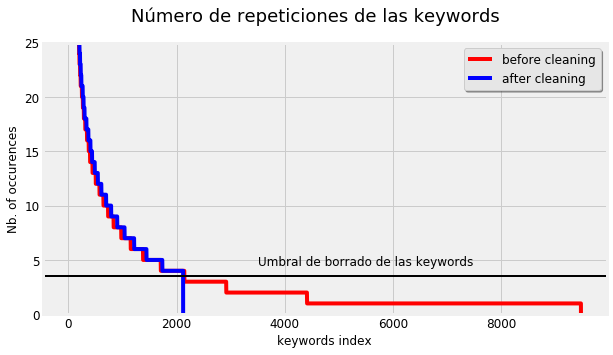
\includegraphics[width=10cm]{./contenido/imagenes/output_62_1.png}

\end{figure}
    { \hspace*{\fill} \\}
    
    \begin{center}\rule{0.5\linewidth}{\linethickness}\end{center}

\subsubsection{2.3 Correlaciones}\label{correlaciones}

    \begin{tcolorbox}[breakable, size=fbox, boxrule=1pt, pad at break*=1mm,colback=cellbackground, colframe=cellborder]
\prompt{In}{incolor}{42}{\hspace{4pt}}
\begin{Verbatim}[commandchars=\\\{\}]
\PY{n}{f}\PY{p}{,} \PY{n}{ax} \PY{o}{=} \PY{n}{plt}\PY{o}{.}\PY{n}{subplots}\PY{p}{(}\PY{n}{figsize}\PY{o}{=}\PY{p}{(}\PY{l+m+mi}{12}\PY{p}{,} \PY{l+m+mi}{9}\PY{p}{)}\PY{p}{)}
\PY{c+c1}{\PYZsh{}\PYZus{}\PYZus{}\PYZus{}\PYZus{}\PYZus{}\PYZus{}\PYZus{}\PYZus{}\PYZus{}\PYZus{}\PYZus{}\PYZus{}\PYZus{}\PYZus{}\PYZus{}\PYZus{}\PYZus{}\PYZus{}\PYZus{}\PYZus{}\PYZus{}\PYZus{}\PYZus{}\PYZus{}\PYZus{}\PYZus{}\PYZus{}\PYZus{}\PYZus{}}
\PY{c+c1}{\PYZsh{} Cálculo de correlaciones}
\PY{n}{corrmat} \PY{o}{=} \PY{n}{df\PYZus{}keywords\PYZus{}occurence}\PY{o}{.}\PY{n}{dropna}\PY{p}{(}\PY{n}{how}\PY{o}{=}\PY{l+s+s1}{\PYZsq{}}\PY{l+s+s1}{any}\PY{l+s+s1}{\PYZsq{}}\PY{p}{)}\PY{o}{.}\PY{n}{corr}\PY{p}{(}\PY{p}{)}
\PY{c+c1}{\PYZsh{}\PYZus{}\PYZus{}\PYZus{}\PYZus{}\PYZus{}\PYZus{}\PYZus{}\PYZus{}\PYZus{}\PYZus{}\PYZus{}\PYZus{}\PYZus{}\PYZus{}\PYZus{}\PYZus{}\PYZus{}\PYZus{}\PYZus{}\PYZus{}\PYZus{}\PYZus{}\PYZus{}\PYZus{}\PYZus{}\PYZus{}\PYZus{}\PYZus{}\PYZus{}\PYZus{}\PYZus{}\PYZus{}\PYZus{}\PYZus{}\PYZus{}\PYZus{}\PYZus{}\PYZus{}\PYZus{}\PYZus{}}
\PY{n}{k} \PY{o}{=} \PY{l+m+mi}{17} \PY{c+c1}{\PYZsh{} number of variables for heatmap}
\PY{n}{cols} \PY{o}{=} \PY{n}{corrmat}\PY{o}{.}\PY{n}{nlargest}\PY{p}{(}\PY{n}{k}\PY{p}{,} \PY{l+s+s1}{\PYZsq{}}\PY{l+s+s1}{num\PYZus{}voted\PYZus{}users}\PY{l+s+s1}{\PYZsq{}}\PY{p}{)}\PY{p}{[}\PY{l+s+s1}{\PYZsq{}}\PY{l+s+s1}{num\PYZus{}voted\PYZus{}users}\PY{l+s+s1}{\PYZsq{}}\PY{p}{]}\PY{o}{.}\PY{n}{index}
\PY{n}{cm} \PY{o}{=} \PY{n}{np}\PY{o}{.}\PY{n}{corrcoef}\PY{p}{(}\PY{n}{df\PYZus{}keywords\PYZus{}occurence}\PY{p}{[}\PY{n}{cols}\PY{p}{]}\PY{o}{.}\PY{n}{dropna}\PY{p}{(}\PY{n}{how}\PY{o}{=}\PY{l+s+s1}{\PYZsq{}}\PY{l+s+s1}{any}\PY{l+s+s1}{\PYZsq{}}\PY{p}{)}\PY{o}{.}\PY{n}{values}\PY{o}{.}\PY{n}{T}\PY{p}{)}
\PY{n}{sns}\PY{o}{.}\PY{n}{set}\PY{p}{(}\PY{n}{font\PYZus{}scale}\PY{o}{=}\PY{l+m+mi}{1}\PY{p}{)}
\PY{n}{hm} \PY{o}{=} \PY{n}{sns}\PY{o}{.}\PY{n}{heatmap}\PY{p}{(}\PY{n}{cm}\PY{p}{,} \PY{n}{cbar}\PY{o}{=}\PY{k+kc}{True}\PY{p}{,} \PY{n}{annot}\PY{o}{=}\PY{k+kc}{True}\PY{p}{,} \PY{n}{square}\PY{o}{=}\PY{k+kc}{True}\PY{p}{,}
                 \PY{n}{fmt}\PY{o}{=}\PY{l+s+s1}{\PYZsq{}}\PY{l+s+s1}{.2f}\PY{l+s+s1}{\PYZsq{}}\PY{p}{,} \PY{n}{annot\PYZus{}kws}\PY{o}{=}\PY{p}{\PYZob{}}\PY{l+s+s1}{\PYZsq{}}\PY{l+s+s1}{size}\PY{l+s+s1}{\PYZsq{}}\PY{p}{:} \PY{l+m+mi}{12}\PY{p}{\PYZcb{}}\PY{p}{,} \PY{n}{linewidth} \PY{o}{=} \PY{l+m+mf}{0.1}\PY{p}{,} \PY{n}{cmap} \PY{o}{=} \PY{l+s+s1}{\PYZsq{}}\PY{l+s+s1}{coolwarm}\PY{l+s+s1}{\PYZsq{}}\PY{p}{,}
                 \PY{n}{yticklabels}\PY{o}{=}\PY{n}{cols}\PY{o}{.}\PY{n}{values}\PY{p}{,} \PY{n}{xticklabels}\PY{o}{=}\PY{n}{cols}\PY{o}{.}\PY{n}{values}\PY{p}{)}
\PY{n}{f}\PY{o}{.}\PY{n}{text}\PY{p}{(}\PY{l+m+mf}{0.5}\PY{p}{,} \PY{l+m+mf}{0.93}\PY{p}{,} \PY{l+s+s2}{\PYZdq{}}\PY{l+s+s2}{Coeficientes de correlación}\PY{l+s+s2}{\PYZdq{}}\PY{p}{,} \PY{n}{ha}\PY{o}{=}\PY{l+s+s1}{\PYZsq{}}\PY{l+s+s1}{center}\PY{l+s+s1}{\PYZsq{}}\PY{p}{,} \PY{n}{fontsize} \PY{o}{=} \PY{l+m+mi}{18}\PY{p}{,} \PY{n}{family}\PY{o}{=}\PY{l+s+s1}{\PYZsq{}}\PY{l+s+s1}{sans\PYZhy{}serif}\PY{l+s+s1}{\PYZsq{}}\PY{p}{)}
\PY{n}{plt}\PY{o}{.}\PY{n}{show}\PY{p}{(}\PY{p}{)}
\end{Verbatim}
\end{tcolorbox}

\begin{figure}[h]
    \centering
    \captionsetup{width=10cm}
    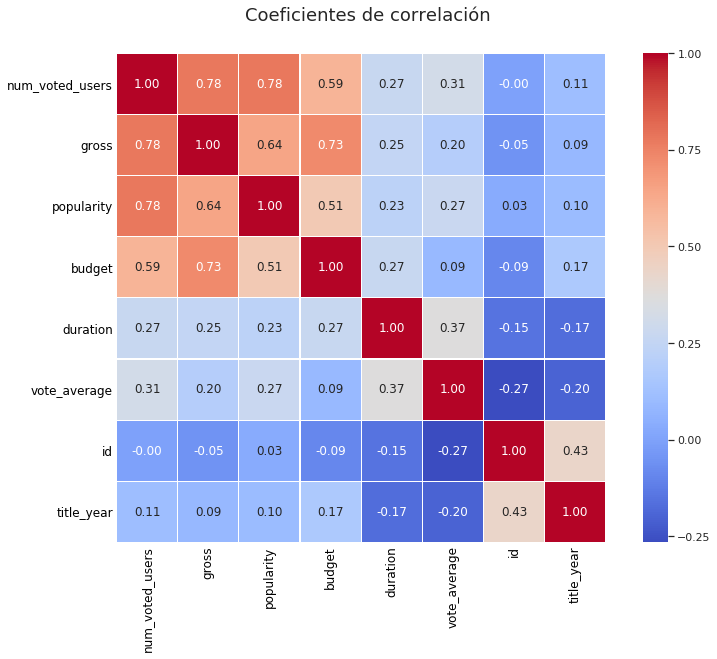
\includegraphics[width=10cm]{./contenido/imagenes/output_64_0.png}

\end{figure}
    { \hspace*{\fill} \\}
    
    \begin{tcolorbox}[breakable, size=fbox, boxrule=1pt, pad at break*=1mm,colback=cellbackground, colframe=cellborder]
\prompt{In}{incolor}{43}{\hspace{4pt}}
\begin{Verbatim}[commandchars=\\\{\}]
\PY{n}{LOST\PYZus{}COLUMNS} \PY{o}{=} \PY{p}{[}
    \PY{l+s+s1}{\PYZsq{}}\PY{l+s+s1}{actor\PYZus{}1\PYZus{}facebook\PYZus{}likes}\PY{l+s+s1}{\PYZsq{}}\PY{p}{,}
    \PY{l+s+s1}{\PYZsq{}}\PY{l+s+s1}{actor\PYZus{}2\PYZus{}facebook\PYZus{}likes}\PY{l+s+s1}{\PYZsq{}}\PY{p}{,}
    \PY{l+s+s1}{\PYZsq{}}\PY{l+s+s1}{actor\PYZus{}3\PYZus{}facebook\PYZus{}likes}\PY{l+s+s1}{\PYZsq{}}\PY{p}{,}
    \PY{l+s+s1}{\PYZsq{}}\PY{l+s+s1}{aspect\PYZus{}ratio}\PY{l+s+s1}{\PYZsq{}}\PY{p}{,}
    \PY{l+s+s1}{\PYZsq{}}\PY{l+s+s1}{cast\PYZus{}total\PYZus{}facebook\PYZus{}likes}\PY{l+s+s1}{\PYZsq{}}\PY{p}{,}
    \PY{l+s+s1}{\PYZsq{}}\PY{l+s+s1}{color}\PY{l+s+s1}{\PYZsq{}}\PY{p}{,}
    \PY{l+s+s1}{\PYZsq{}}\PY{l+s+s1}{content\PYZus{}rating}\PY{l+s+s1}{\PYZsq{}}\PY{p}{,}
    \PY{l+s+s1}{\PYZsq{}}\PY{l+s+s1}{director\PYZus{}facebook\PYZus{}likes}\PY{l+s+s1}{\PYZsq{}}\PY{p}{,}
    \PY{l+s+s1}{\PYZsq{}}\PY{l+s+s1}{facenumber\PYZus{}in\PYZus{}poster}\PY{l+s+s1}{\PYZsq{}}\PY{p}{,}
    \PY{l+s+s1}{\PYZsq{}}\PY{l+s+s1}{movie\PYZus{}facebook\PYZus{}likes}\PY{l+s+s1}{\PYZsq{}}\PY{p}{,}
    \PY{l+s+s1}{\PYZsq{}}\PY{l+s+s1}{movie\PYZus{}imdb\PYZus{}link}\PY{l+s+s1}{\PYZsq{}}\PY{p}{,}
    \PY{l+s+s1}{\PYZsq{}}\PY{l+s+s1}{num\PYZus{}critic\PYZus{}for\PYZus{}reviews}\PY{l+s+s1}{\PYZsq{}}\PY{p}{,}
    \PY{l+s+s1}{\PYZsq{}}\PY{l+s+s1}{num\PYZus{}user\PYZus{}for\PYZus{}reviews}\PY{l+s+s1}{\PYZsq{}}
                \PY{p}{]}
\end{Verbatim}
\end{tcolorbox}

    \begin{tcolorbox}[breakable, size=fbox, boxrule=1pt, pad at break*=1mm,colback=cellbackground, colframe=cellborder]
\prompt{In}{incolor}{44}{\hspace{4pt}}
\begin{Verbatim}[commandchars=\\\{\}]
\PY{c+c1}{\PYZsh{}\PYZus{}\PYZus{}\PYZus{}\PYZus{}\PYZus{}\PYZus{}\PYZus{}\PYZus{}\PYZus{}\PYZus{}}
\PY{c+c1}{\PYZsh{} dropping}
\PY{c+c1}{\PYZsh{}dropped\PYZus{}var = [\PYZsq{}aspect\PYZus{}ratio\PYZsq{}, \PYZsq{}budget\PYZsq{}, \PYZsq{}facenumber\PYZus{}in\PYZus{}poster\PYZsq{},}
\PY{c+c1}{\PYZsh{}               \PYZsq{}content\PYZus{}rating\PYZsq{}, \PYZsq{}cast\PYZus{}total\PYZus{}facebook\PYZus{}likes\PYZsq{}]}
\PY{c+c1}{\PYZsh{}df\PYZus{}var\PYZus{}cleaned = df\PYZus{}keywords\PYZus{}occurence.drop(dropped\PYZus{}var, axis = 1)}
\PY{c+c1}{\PYZsh{}\PYZus{}\PYZus{}\PYZus{}\PYZus{}\PYZus{}\PYZus{}\PYZus{}\PYZus{}\PYZus{}\PYZus{}\PYZus{}\PYZus{}\PYZus{}\PYZus{}\PYZus{}\PYZus{}}
\PY{c+c1}{\PYZsh{} and reordering}
\PY{n}{new\PYZus{}col\PYZus{}order} \PY{o}{=} \PY{p}{[}\PY{l+s+s1}{\PYZsq{}}\PY{l+s+s1}{movie\PYZus{}title}\PY{l+s+s1}{\PYZsq{}}\PY{p}{,} \PY{l+s+s1}{\PYZsq{}}\PY{l+s+s1}{title\PYZus{}year}\PY{l+s+s1}{\PYZsq{}}\PY{p}{,} \PY{l+s+s1}{\PYZsq{}}\PY{l+s+s1}{genres}\PY{l+s+s1}{\PYZsq{}}\PY{p}{,} \PY{l+s+s1}{\PYZsq{}}\PY{l+s+s1}{plot\PYZus{}keywords}\PY{l+s+s1}{\PYZsq{}}\PY{p}{,} 
                 \PY{l+s+s1}{\PYZsq{}}\PY{l+s+s1}{director\PYZus{}name}\PY{l+s+s1}{\PYZsq{}}\PY{p}{,} \PY{l+s+s1}{\PYZsq{}}\PY{l+s+s1}{actor\PYZus{}1\PYZus{}name}\PY{l+s+s1}{\PYZsq{}}\PY{p}{,} \PY{l+s+s1}{\PYZsq{}}\PY{l+s+s1}{actor\PYZus{}2\PYZus{}name}\PY{l+s+s1}{\PYZsq{}}\PY{p}{,} \PY{l+s+s1}{\PYZsq{}}\PY{l+s+s1}{actor\PYZus{}3\PYZus{}name}\PY{l+s+s1}{\PYZsq{}}\PY{p}{,}
                 \PY{l+s+s1}{\PYZsq{}}\PY{l+s+s1}{director\PYZus{}facebook\PYZus{}likes}\PY{l+s+s1}{\PYZsq{}}\PY{p}{,} \PY{l+s+s1}{\PYZsq{}}\PY{l+s+s1}{actor\PYZus{}1\PYZus{}facebook\PYZus{}likes}\PY{l+s+s1}{\PYZsq{}}\PY{p}{,} \PY{l+s+s1}{\PYZsq{}}\PY{l+s+s1}{actor\PYZus{}2\PYZus{}facebook\PYZus{}likes}\PY{l+s+s1}{\PYZsq{}}\PY{p}{,}
                 \PY{l+s+s1}{\PYZsq{}}\PY{l+s+s1}{actor\PYZus{}3\PYZus{}facebook\PYZus{}likes}\PY{l+s+s1}{\PYZsq{}}\PY{p}{,} \PY{l+s+s1}{\PYZsq{}}\PY{l+s+s1}{movie\PYZus{}facebook\PYZus{}likes}\PY{l+s+s1}{\PYZsq{}}\PY{p}{,} \PY{l+s+s1}{\PYZsq{}}\PY{l+s+s1}{num\PYZus{}critic\PYZus{}for\PYZus{}reviews}\PY{l+s+s1}{\PYZsq{}}\PY{p}{,} 
                 \PY{l+s+s1}{\PYZsq{}}\PY{l+s+s1}{num\PYZus{}user\PYZus{}for\PYZus{}reviews}\PY{l+s+s1}{\PYZsq{}}\PY{p}{,} \PY{l+s+s1}{\PYZsq{}}\PY{l+s+s1}{num\PYZus{}voted\PYZus{}users}\PY{l+s+s1}{\PYZsq{}}\PY{p}{,} \PY{l+s+s1}{\PYZsq{}}\PY{l+s+s1}{language}\PY{l+s+s1}{\PYZsq{}}\PY{p}{,} \PY{l+s+s1}{\PYZsq{}}\PY{l+s+s1}{country}\PY{l+s+s1}{\PYZsq{}}\PY{p}{,}
                 \PY{l+s+s1}{\PYZsq{}}\PY{l+s+s1}{imdb\PYZus{}score}\PY{l+s+s1}{\PYZsq{}}\PY{p}{,} \PY{l+s+s1}{\PYZsq{}}\PY{l+s+s1}{movie\PYZus{}imdb\PYZus{}link}\PY{l+s+s1}{\PYZsq{}}\PY{p}{,} \PY{l+s+s1}{\PYZsq{}}\PY{l+s+s1}{color}\PY{l+s+s1}{\PYZsq{}}\PY{p}{,} \PY{l+s+s1}{\PYZsq{}}\PY{l+s+s1}{duration}\PY{l+s+s1}{\PYZsq{}}\PY{p}{,} \PY{l+s+s1}{\PYZsq{}}\PY{l+s+s1}{gross}\PY{l+s+s1}{\PYZsq{}}\PY{p}{,} \PY{p}{]}
\PY{n}{new\PYZus{}col\PYZus{}order} \PY{o}{=} \PY{p}{[}\PY{n}{col} \PY{k}{for} \PY{n}{col} \PY{o+ow}{in} \PY{n}{new\PYZus{}col\PYZus{}order} \PY{k}{if} \PY{n}{col} \PY{o+ow}{not} \PY{o+ow}{in} \PY{n}{LOST\PYZus{}COLUMNS}\PY{p}{]}
\PY{n+nb}{print}\PY{p}{(}\PY{n}{new\PYZus{}col\PYZus{}order}\PY{p}{)}
\PY{n}{new\PYZus{}col\PYZus{}order} \PY{o}{=} \PY{p}{[}\PY{n}{IMDB\PYZus{}COLUMNS\PYZus{}TO\PYZus{}REMAP}\PY{p}{[}\PY{n}{col}\PY{p}{]} \PY{k}{if} \PY{n}{col} \PY{o+ow}{in} \PY{n}{IMDB\PYZus{}COLUMNS\PYZus{}TO\PYZus{}REMAP} \PY{k}{else} \PY{n}{col}
                 \PY{k}{for} \PY{n}{col} \PY{o+ow}{in} \PY{n}{new\PYZus{}col\PYZus{}order}\PY{p}{]}
\PY{n+nb}{print}\PY{p}{(}\PY{n}{new\PYZus{}col\PYZus{}order}\PY{p}{)}
\PY{n}{new\PYZus{}col\PYZus{}order} \PY{o}{=} \PY{p}{[}\PY{n}{TMDB\PYZus{}TO\PYZus{}IMDB\PYZus{}SIMPLE\PYZus{}EQUIVALENCIES}\PY{p}{[}\PY{n}{col}\PY{p}{]} \PY{k}{if} \PY{n}{col} \PY{o+ow}{in} \PY{n}{TMDB\PYZus{}TO\PYZus{}IMDB\PYZus{}SIMPLE\PYZus{}EQUIVALENCIES} \PY{k}{else} \PY{n}{col}
                 \PY{k}{for} \PY{n}{col} \PY{o+ow}{in} \PY{n}{new\PYZus{}col\PYZus{}order}\PY{p}{]}
\PY{n+nb}{print}\PY{p}{(}\PY{n}{new\PYZus{}col\PYZus{}order}\PY{p}{)}
\PY{n}{df\PYZus{}var\PYZus{}cleaned} \PY{o}{=} \PY{n}{df\PYZus{}keywords\PYZus{}occurence}\PY{p}{[}\PY{n}{new\PYZus{}col\PYZus{}order}\PY{p}{]}
\end{Verbatim}
\end{tcolorbox}

    \begin{Verbatim}[commandchars=\\\{\}]
['movie\_title', 'title\_year', 'genres', 'plot\_keywords', 'director\_name',
'actor\_1\_name', 'actor\_2\_name', 'actor\_3\_name', 'num\_voted\_users', 'language',
'country', 'imdb\_score', 'duration', 'gross']
['movie\_title', 'title\_year', 'genres', 'plot\_keywords', 'director\_name',
'actor\_1\_name', 'actor\_2\_name', 'actor\_3\_name', 'num\_voted\_users', 'language',
'country', 'vote\_average', 'duration', 'gross']
['movie\_title', 'title\_year', 'genres', 'plot\_keywords', 'director\_name',
'actor\_1\_name', 'actor\_2\_name', 'actor\_3\_name', 'num\_voted\_users', 'language',
'country', 'vote\_average', 'duration', 'gross']
\end{Verbatim}

    \begin{tcolorbox}[breakable, size=fbox, boxrule=1pt, pad at break*=1mm,colback=cellbackground, colframe=cellborder]
\prompt{In}{incolor}{45}{\hspace{4pt}}
\begin{Verbatim}[commandchars=\\\{\}]
\PY{n}{set2} \PY{o}{=} \PY{n+nb}{set}\PY{p}{(}\PY{n+nb}{list}\PY{p}{(}\PY{n}{df\PYZus{}var\PYZus{}cleaned}\PY{o}{.}\PY{n}{columns}\PY{p}{)}\PY{p}{)}
\end{Verbatim}
\end{tcolorbox}

    \begin{tcolorbox}[breakable, size=fbox, boxrule=1pt, pad at break*=1mm,colback=cellbackground, colframe=cellborder]
\prompt{In}{incolor}{46}{\hspace{4pt}}
\begin{Verbatim}[commandchars=\\\{\}]
\PY{n}{set1} \PY{o}{=} \PY{n+nb}{set}\PY{p}{(}\PY{n+nb}{list}\PY{p}{(}\PY{n}{df\PYZus{}keywords\PYZus{}occurence}\PY{o}{.}\PY{n}{columns}\PY{p}{)}\PY{p}{)}
\PY{n}{set1}\PY{o}{.}\PY{n}{difference}\PY{p}{(}\PY{n+nb}{list}\PY{p}{(}\PY{n}{df\PYZus{}var\PYZus{}cleaned}\PY{o}{.}\PY{n}{columns}\PY{p}{)}\PY{p}{)}
\end{Verbatim}
\end{tcolorbox}

            \begin{tcolorbox}[breakable, boxrule=.5pt, size=fbox, pad at break*=1mm, opacityfill=0]
\prompt{Out}{outcolor}{46}{\hspace{3.5pt}}
\begin{Verbatim}[commandchars=\\\{\}]
\{'budget',
 'homepage',
 'id',
 'original\_title',
 'overview',
 'popularity',
 'production\_companies',
 'production\_countries',
 'release\_date',
 'spoken\_languages',
 'status',
 'tagline'\}
\end{Verbatim}
\end{tcolorbox}
        
    \begin{center}\rule{0.5\linewidth}{\linethickness}\end{center}

\subsubsection{2.4 Valores faltantes}\label{valores-faltantes}

Examinamos el número de valores faltantes en cada variable y escogemos
una metodología para completar el dataset.

    \begin{tcolorbox}[breakable, size=fbox, boxrule=1pt, pad at break*=1mm,colback=cellbackground, colframe=cellborder]
\prompt{In}{incolor}{47}{\hspace{4pt}}
\begin{Verbatim}[commandchars=\\\{\}]
\PY{n}{missing\PYZus{}df} \PY{o}{=} \PY{n}{df\PYZus{}var\PYZus{}cleaned}\PY{o}{.}\PY{n}{isnull}\PY{p}{(}\PY{p}{)}\PY{o}{.}\PY{n}{sum}\PY{p}{(}\PY{n}{axis}\PY{o}{=}\PY{l+m+mi}{0}\PY{p}{)}\PY{o}{.}\PY{n}{reset\PYZus{}index}\PY{p}{(}\PY{p}{)}
\PY{n}{missing\PYZus{}df}\PY{o}{.}\PY{n}{columns} \PY{o}{=} \PY{p}{[}\PY{l+s+s1}{\PYZsq{}}\PY{l+s+s1}{column\PYZus{}name}\PY{l+s+s1}{\PYZsq{}}\PY{p}{,} \PY{l+s+s1}{\PYZsq{}}\PY{l+s+s1}{missing\PYZus{}count}\PY{l+s+s1}{\PYZsq{}}\PY{p}{]}
\PY{n}{missing\PYZus{}df}\PY{p}{[}\PY{l+s+s1}{\PYZsq{}}\PY{l+s+s1}{filling\PYZus{}factor}\PY{l+s+s1}{\PYZsq{}}\PY{p}{]} \PY{o}{=} \PY{p}{(}\PY{n}{df\PYZus{}var\PYZus{}cleaned}\PY{o}{.}\PY{n}{shape}\PY{p}{[}\PY{l+m+mi}{0}\PY{p}{]} 
                                \PY{o}{\PYZhy{}} \PY{n}{missing\PYZus{}df}\PY{p}{[}\PY{l+s+s1}{\PYZsq{}}\PY{l+s+s1}{missing\PYZus{}count}\PY{l+s+s1}{\PYZsq{}}\PY{p}{]}\PY{p}{)} \PY{o}{/} \PY{n}{df\PYZus{}var\PYZus{}cleaned}\PY{o}{.}\PY{n}{shape}\PY{p}{[}\PY{l+m+mi}{0}\PY{p}{]} \PY{o}{*} \PY{l+m+mi}{100}
\PY{n}{missing\PYZus{}df} \PY{o}{=} \PY{n}{missing\PYZus{}df}\PY{o}{.}\PY{n}{sort\PYZus{}values}\PY{p}{(}\PY{l+s+s1}{\PYZsq{}}\PY{l+s+s1}{filling\PYZus{}factor}\PY{l+s+s1}{\PYZsq{}}\PY{p}{)}\PY{o}{.}\PY{n}{reset\PYZus{}index}\PY{p}{(}\PY{n}{drop} \PY{o}{=} \PY{k+kc}{True}\PY{p}{)}
\PY{n}{missing\PYZus{}df}
\end{Verbatim}
\end{tcolorbox}

            \begin{tcolorbox}[breakable, boxrule=.5pt, size=fbox, pad at break*=1mm, opacityfill=0]
\prompt{Out}{outcolor}{47}{\hspace{3.5pt}}
\begin{Verbatim}[commandchars=\\\{\}]
        column\_name  missing\_count  filling\_factor
0           country            174       96.377264
1      actor\_3\_name             93       98.063710
2          language             86       98.209452
3      actor\_2\_name             63       98.688320
4      actor\_1\_name             53       98.896523
5     director\_name             30       99.375390
6          duration              2       99.958359
7        title\_year              1       99.979180
8       movie\_title              0      100.000000
9            genres              0      100.000000
10    plot\_keywords              0      100.000000
11  num\_voted\_users              0      100.000000
12     vote\_average              0      100.000000
13            gross              0      100.000000
\end{Verbatim}
\end{tcolorbox}
        
    Ahora representamos el contenido de esta tabla:

    \begin{tcolorbox}[breakable, size=fbox, boxrule=1pt, pad at break*=1mm,colback=cellbackground, colframe=cellborder]
\prompt{In}{incolor}{48}{\hspace{4pt}}
\begin{Verbatim}[commandchars=\\\{\}]
\PY{n}{y\PYZus{}axis} \PY{o}{=} \PY{n}{missing\PYZus{}df}\PY{p}{[}\PY{l+s+s1}{\PYZsq{}}\PY{l+s+s1}{filling\PYZus{}factor}\PY{l+s+s1}{\PYZsq{}}\PY{p}{]} 
\PY{n}{x\PYZus{}label} \PY{o}{=} \PY{n}{missing\PYZus{}df}\PY{p}{[}\PY{l+s+s1}{\PYZsq{}}\PY{l+s+s1}{column\PYZus{}name}\PY{l+s+s1}{\PYZsq{}}\PY{p}{]}
\PY{n}{x\PYZus{}axis} \PY{o}{=} \PY{n}{missing\PYZus{}df}\PY{o}{.}\PY{n}{index}

\PY{n}{fig} \PY{o}{=} \PY{n}{plt}\PY{o}{.}\PY{n}{figure}\PY{p}{(}\PY{n}{figsize}\PY{o}{=}\PY{p}{(}\PY{l+m+mi}{11}\PY{p}{,} \PY{l+m+mi}{4}\PY{p}{)}\PY{p}{)}
\PY{n}{plt}\PY{o}{.}\PY{n}{xticks}\PY{p}{(}\PY{n}{rotation}\PY{o}{=}\PY{l+m+mi}{80}\PY{p}{,} \PY{n}{fontsize} \PY{o}{=} \PY{l+m+mi}{12}\PY{p}{)}
\PY{n}{plt}\PY{o}{.}\PY{n}{yticks}\PY{p}{(}\PY{n}{fontsize} \PY{o}{=} \PY{l+m+mi}{13}\PY{p}{)}

\PY{n}{N\PYZus{}thresh} \PY{o}{=} \PY{l+m+mi}{5}
\PY{n}{plt}\PY{o}{.}\PY{n}{axvline}\PY{p}{(}\PY{n}{x}\PY{o}{=}\PY{n}{N\PYZus{}thresh}\PY{o}{\PYZhy{}}\PY{l+m+mf}{0.5}\PY{p}{,} \PY{n}{linewidth}\PY{o}{=}\PY{l+m+mi}{2}\PY{p}{,} \PY{n}{color} \PY{o}{=} \PY{l+s+s1}{\PYZsq{}}\PY{l+s+s1}{r}\PY{l+s+s1}{\PYZsq{}}\PY{p}{)}
\PY{n}{plt}\PY{o}{.}\PY{n}{text}\PY{p}{(}\PY{n}{N\PYZus{}thresh}\PY{o}{\PYZhy{}}\PY{l+m+mf}{4.8}\PY{p}{,} \PY{l+m+mi}{30}\PY{p}{,} \PY{l+s+s1}{\PYZsq{}}\PY{l+s+s1}{Factor completitud }\PY{l+s+se}{\PYZbs{}n}\PY{l+s+s1}{ \PYZlt{} }\PY{l+s+si}{\PYZob{}\PYZcb{}}\PY{l+s+s1}{\PYZpc{}}\PY{l+s+s1}{\PYZsq{}}\PY{o}{.}\PY{n}{format}\PY{p}{(}\PY{n+nb}{round}\PY{p}{(}\PY{n}{y\PYZus{}axis}\PY{p}{[}\PY{n}{N\PYZus{}thresh}\PY{p}{]}\PY{p}{,}\PY{l+m+mi}{1}\PY{p}{)}\PY{p}{)}\PY{p}{,}
         \PY{n}{fontsize} \PY{o}{=} \PY{l+m+mi}{15}\PY{p}{,} \PY{n}{family} \PY{o}{=} \PY{l+s+s1}{\PYZsq{}}\PY{l+s+s1}{sans\PYZhy{}serif}\PY{l+s+s1}{\PYZsq{}}\PY{p}{,} \PY{n}{bbox}\PY{o}{=}\PY{n+nb}{dict}\PY{p}{(}\PY{n}{boxstyle}\PY{o}{=}\PY{l+s+s2}{\PYZdq{}}\PY{l+s+s2}{round}\PY{l+s+s2}{\PYZdq{}}\PY{p}{,}
                   \PY{n}{ec}\PY{o}{=}\PY{p}{(}\PY{l+m+mf}{1.0}\PY{p}{,} \PY{l+m+mf}{0.5}\PY{p}{,} \PY{l+m+mf}{0.5}\PY{p}{)}\PY{p}{,}
                   \PY{n}{fc}\PY{o}{=}\PY{p}{(}\PY{l+m+mf}{0.8}\PY{p}{,} \PY{l+m+mf}{0.5}\PY{p}{,} \PY{l+m+mf}{0.5}\PY{p}{)}\PY{p}{)}\PY{p}{)}
\PY{n}{N\PYZus{}thresh} \PY{o}{=} \PY{l+m+mi}{13}
\PY{n}{plt}\PY{o}{.}\PY{n}{axvline}\PY{p}{(}\PY{n}{x}\PY{o}{=}\PY{n}{N\PYZus{}thresh}\PY{o}{\PYZhy{}}\PY{l+m+mf}{0.5}\PY{p}{,} \PY{n}{linewidth}\PY{o}{=}\PY{l+m+mi}{2}\PY{p}{,} \PY{n}{color} \PY{o}{=} \PY{l+s+s1}{\PYZsq{}}\PY{l+s+s1}{g}\PY{l+s+s1}{\PYZsq{}}\PY{p}{)}
\PY{n}{plt}\PY{o}{.}\PY{n}{text}\PY{p}{(}\PY{n}{N\PYZus{}thresh}\PY{p}{,} \PY{l+m+mi}{30}\PY{p}{,} \PY{l+s+s1}{\PYZsq{}}\PY{l+s+s1}{Factor completitud }\PY{l+s+se}{\PYZbs{}n}\PY{l+s+s1}{ = }\PY{l+s+si}{\PYZob{}\PYZcb{}}\PY{l+s+s1}{\PYZpc{}}\PY{l+s+s1}{\PYZsq{}}\PY{o}{.}\PY{n}{format}\PY{p}{(}\PY{n+nb}{round}\PY{p}{(}\PY{n}{y\PYZus{}axis}\PY{p}{[}\PY{n}{N\PYZus{}thresh}\PY{p}{]}\PY{p}{,}\PY{l+m+mi}{1}\PY{p}{)}\PY{p}{)}\PY{p}{,}
         \PY{n}{fontsize} \PY{o}{=} \PY{l+m+mi}{15}\PY{p}{,} \PY{n}{family} \PY{o}{=} \PY{l+s+s1}{\PYZsq{}}\PY{l+s+s1}{sans\PYZhy{}serif}\PY{l+s+s1}{\PYZsq{}}\PY{p}{,} \PY{n}{bbox}\PY{o}{=}\PY{n+nb}{dict}\PY{p}{(}\PY{n}{boxstyle}\PY{o}{=}\PY{l+s+s2}{\PYZdq{}}\PY{l+s+s2}{round}\PY{l+s+s2}{\PYZdq{}}\PY{p}{,}
                   \PY{n}{ec}\PY{o}{=}\PY{p}{(}\PY{l+m+mf}{0.5}\PY{p}{,} \PY{l+m+mf}{1.}\PY{p}{,} \PY{l+m+mf}{0.5}\PY{p}{)}\PY{p}{,}
                   \PY{n}{fc}\PY{o}{=}\PY{p}{(}\PY{l+m+mf}{0.5}\PY{p}{,} \PY{l+m+mf}{0.8}\PY{p}{,} \PY{l+m+mf}{0.5}\PY{p}{)}\PY{p}{)}\PY{p}{)}

\PY{n}{plt}\PY{o}{.}\PY{n}{xticks}\PY{p}{(}\PY{n}{x\PYZus{}axis}\PY{p}{,} \PY{n}{x\PYZus{}label}\PY{p}{,}\PY{n}{family}\PY{o}{=}\PY{l+s+s1}{\PYZsq{}}\PY{l+s+s1}{sans\PYZhy{}serif}\PY{l+s+s1}{\PYZsq{}}\PY{p}{,} \PY{n}{fontsize} \PY{o}{=} \PY{l+m+mi}{14} \PY{p}{)}
\PY{n}{plt}\PY{o}{.}\PY{n}{ylabel}\PY{p}{(}\PY{l+s+s1}{\PYZsq{}}\PY{l+s+s1}{Factor de completitud (}\PY{l+s+s1}{\PYZpc{}}\PY{l+s+s1}{)}\PY{l+s+s1}{\PYZsq{}}\PY{p}{,} \PY{n}{family}\PY{o}{=}\PY{l+s+s1}{\PYZsq{}}\PY{l+s+s1}{sans\PYZhy{}serif}\PY{l+s+s1}{\PYZsq{}}\PY{p}{,} \PY{n}{fontsize} \PY{o}{=} \PY{l+m+mi}{12}\PY{p}{)}
\PY{n}{plt}\PY{o}{.}\PY{n}{bar}\PY{p}{(}\PY{n}{x\PYZus{}axis}\PY{p}{,} \PY{n}{y\PYZus{}axis}\PY{p}{)}\PY{p}{;}
\end{Verbatim}
\end{tcolorbox}

\begin{figure}[h]
    \centering
    \captionsetup{width=10cm}
    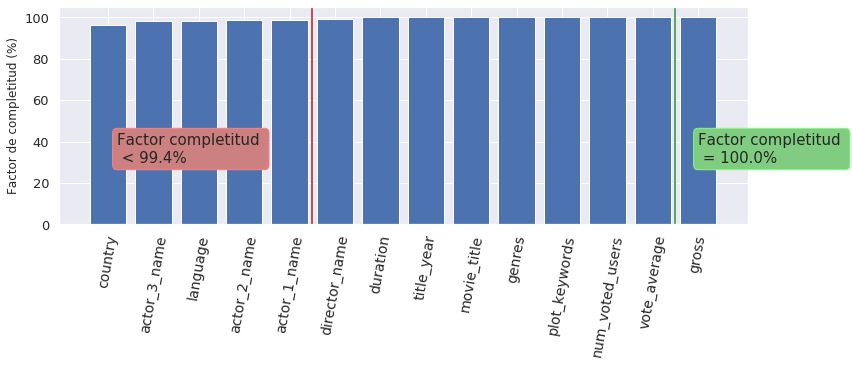
\includegraphics[width=10cm]{./contenido/imagenes/output_72_0.png}

\end{figure}
    { \hspace*{\fill} \\}
    
    \begin{center}\rule{0.5\linewidth}{\linethickness}\end{center}

\paragraph{2.4.1 Completando los años
faltantes}\label{completando-los-auxf1os-faltantes}

Para inferir el año de la película, se usan los actores y el director.
Para cada uno de ellos, determinamos el año medio de actividad,
utilizando el dataset que tenemos. A continuación, se promedian los
valores para determinar el año de la película.

    \begin{tcolorbox}[breakable, size=fbox, boxrule=1pt, pad at break*=1mm,colback=cellbackground, colframe=cellborder]
\prompt{In}{incolor}{49}{\hspace{4pt}}
\begin{Verbatim}[commandchars=\\\{\}]
\PY{k}{def} \PY{n+nf}{fill\PYZus{}year}\PY{p}{(}\PY{n}{df}\PY{p}{)}\PY{p}{:}
    \PY{l+s+sd}{\PYZdq{}\PYZdq{}\PYZdq{}Completa la columna faltante del año teniendo en cuenta la media}
\PY{l+s+sd}{    de los periodos de actividad de los actores y el director.}
\PY{l+s+sd}{    \PYZdq{}\PYZdq{}\PYZdq{}}
    \PY{n}{col} \PY{o}{=} \PY{p}{[}\PY{l+s+s1}{\PYZsq{}}\PY{l+s+s1}{director\PYZus{}name}\PY{l+s+s1}{\PYZsq{}}\PY{p}{,} \PY{l+s+s1}{\PYZsq{}}\PY{l+s+s1}{actor\PYZus{}1\PYZus{}name}\PY{l+s+s1}{\PYZsq{}}\PY{p}{,} \PY{l+s+s1}{\PYZsq{}}\PY{l+s+s1}{actor\PYZus{}2\PYZus{}name}\PY{l+s+s1}{\PYZsq{}}\PY{p}{,} \PY{l+s+s1}{\PYZsq{}}\PY{l+s+s1}{actor\PYZus{}3\PYZus{}name}\PY{l+s+s1}{\PYZsq{}}\PY{p}{]}
    \PY{n}{usual\PYZus{}year} \PY{o}{=} \PY{p}{[}\PY{l+m+mi}{0} \PY{k}{for} \PY{n}{\PYZus{}} \PY{o+ow}{in} \PY{n+nb}{range}\PY{p}{(}\PY{l+m+mi}{4}\PY{p}{)}\PY{p}{]}
    \PY{n}{var}        \PY{o}{=} \PY{p}{[}\PY{l+m+mi}{0} \PY{k}{for} \PY{n}{\PYZus{}} \PY{o+ow}{in} \PY{n+nb}{range}\PY{p}{(}\PY{l+m+mi}{4}\PY{p}{)}\PY{p}{]}
    \PY{c+c1}{\PYZsh{}\PYZus{}\PYZus{}\PYZus{}\PYZus{}\PYZus{}\PYZus{}\PYZus{}\PYZus{}\PYZus{}\PYZus{}\PYZus{}\PYZus{}\PYZus{}\PYZus{}\PYZus{}\PYZus{}\PYZus{}\PYZus{}\PYZus{}\PYZus{}\PYZus{}\PYZus{}\PYZus{}\PYZus{}\PYZus{}\PYZus{}\PYZus{}\PYZus{}\PYZus{}\PYZus{}\PYZus{}\PYZus{}\PYZus{}\PYZus{}\PYZus{}\PYZus{}\PYZus{}\PYZus{}\PYZus{}\PYZus{}\PYZus{}\PYZus{}\PYZus{}\PYZus{}\PYZus{}\PYZus{}\PYZus{}\PYZus{}\PYZus{}\PYZus{}\PYZus{}\PYZus{}\PYZus{}\PYZus{}\PYZus{}\PYZus{}\PYZus{}\PYZus{}\PYZus{}\PYZus{}\PYZus{}}
    \PY{c+c1}{\PYZsh{} Año medio de actividad para los actores y el director}
    \PY{k}{for} \PY{n}{i} \PY{o+ow}{in} \PY{n+nb}{range}\PY{p}{(}\PY{n+nb}{len}\PY{p}{(}\PY{n}{col}\PY{p}{)}\PY{p}{)}\PY{p}{:}
        \PY{n}{usual\PYZus{}year}\PY{p}{[}\PY{n}{i}\PY{p}{]} \PY{o}{=} \PY{n}{df}\PY{o}{.}\PY{n}{groupby}\PY{p}{(}\PY{n}{col}\PY{p}{[}\PY{n}{i}\PY{p}{]}\PY{p}{)}\PY{p}{[}\PY{l+s+s1}{\PYZsq{}}\PY{l+s+s1}{title\PYZus{}year}\PY{l+s+s1}{\PYZsq{}}\PY{p}{]}\PY{o}{.}\PY{n}{mean}\PY{p}{(}\PY{p}{)}
    \PY{c+c1}{\PYZsh{}\PYZus{}\PYZus{}\PYZus{}\PYZus{}\PYZus{}\PYZus{}\PYZus{}\PYZus{}\PYZus{}\PYZus{}\PYZus{}\PYZus{}\PYZus{}\PYZus{}\PYZus{}\PYZus{}\PYZus{}\PYZus{}\PYZus{}\PYZus{}\PYZus{}\PYZus{}\PYZus{}\PYZus{}\PYZus{}\PYZus{}\PYZus{}\PYZus{}\PYZus{}\PYZus{}\PYZus{}\PYZus{}\PYZus{}\PYZus{}\PYZus{}\PYZus{}\PYZus{}\PYZus{}\PYZus{}\PYZus{}\PYZus{}\PYZus{}\PYZus{}\PYZus{}\PYZus{}}
    \PY{c+c1}{\PYZsh{} Diccionario que recoja esta información}
    \PY{n}{actor\PYZus{}year} \PY{o}{=} \PY{n+nb}{dict}\PY{p}{(}\PY{p}{)}
    \PY{k}{for} \PY{n}{i} \PY{o+ow}{in} \PY{n+nb}{range}\PY{p}{(}\PY{l+m+mi}{4}\PY{p}{)}\PY{p}{:}
        \PY{k}{for} \PY{n}{s} \PY{o+ow}{in} \PY{n}{usual\PYZus{}year}\PY{p}{[}\PY{n}{i}\PY{p}{]}\PY{o}{.}\PY{n}{index}\PY{p}{:}
            \PY{k}{if} \PY{n}{s} \PY{o+ow}{in} \PY{n}{actor\PYZus{}year}\PY{o}{.}\PY{n}{keys}\PY{p}{(}\PY{p}{)}\PY{p}{:}
                \PY{k}{if} \PY{n}{pd}\PY{o}{.}\PY{n}{notnull}\PY{p}{(}\PY{n}{usual\PYZus{}year}\PY{p}{[}\PY{n}{i}\PY{p}{]}\PY{p}{[}\PY{n}{s}\PY{p}{]}\PY{p}{)} \PY{o+ow}{and} \PY{n}{pd}\PY{o}{.}\PY{n}{notnull}\PY{p}{(}\PY{n}{actor\PYZus{}year}\PY{p}{[}\PY{n}{s}\PY{p}{]}\PY{p}{)}\PY{p}{:}
                    \PY{n}{actor\PYZus{}year}\PY{p}{[}\PY{n}{s}\PY{p}{]} \PY{o}{=} \PY{p}{(}\PY{n}{actor\PYZus{}year}\PY{p}{[}\PY{n}{s}\PY{p}{]} \PY{o}{+} \PY{n}{usual\PYZus{}year}\PY{p}{[}\PY{n}{i}\PY{p}{]}\PY{p}{[}\PY{n}{s}\PY{p}{]}\PY{p}{)}\PY{o}{/}\PY{l+m+mi}{2}
                \PY{k}{elif} \PY{n}{pd}\PY{o}{.}\PY{n}{isnull}\PY{p}{(}\PY{n}{actor\PYZus{}year}\PY{p}{[}\PY{n}{s}\PY{p}{]}\PY{p}{)}\PY{p}{:}
                    \PY{n}{actor\PYZus{}year}\PY{p}{[}\PY{n}{s}\PY{p}{]} \PY{o}{=} \PY{n}{usual\PYZus{}year}\PY{p}{[}\PY{n}{i}\PY{p}{]}\PY{p}{[}\PY{n}{s}\PY{p}{]}
            \PY{k}{else}\PY{p}{:}
                \PY{n}{actor\PYZus{}year}\PY{p}{[}\PY{n}{s}\PY{p}{]} \PY{o}{=} \PY{n}{usual\PYZus{}year}\PY{p}{[}\PY{n}{i}\PY{p}{]}\PY{p}{[}\PY{n}{s}\PY{p}{]}
        
    \PY{c+c1}{\PYZsh{}\PYZus{}\PYZus{}\PYZus{}\PYZus{}\PYZus{}\PYZus{}\PYZus{}\PYZus{}\PYZus{}\PYZus{}\PYZus{}\PYZus{}\PYZus{}\PYZus{}\PYZus{}\PYZus{}\PYZus{}\PYZus{}\PYZus{}\PYZus{}\PYZus{}\PYZus{}\PYZus{}\PYZus{}\PYZus{}\PYZus{}\PYZus{}\PYZus{}\PYZus{}\PYZus{}\PYZus{}\PYZus{}\PYZus{}\PYZus{}\PYZus{}\PYZus{}\PYZus{}\PYZus{}}
    \PY{c+c1}{\PYZsh{} Identificación de los años faltantes}
    \PY{n}{missing\PYZus{}year\PYZus{}info} \PY{o}{=} \PY{n}{df}\PY{p}{[}\PY{n}{df}\PY{p}{[}\PY{l+s+s1}{\PYZsq{}}\PY{l+s+s1}{title\PYZus{}year}\PY{l+s+s1}{\PYZsq{}}\PY{p}{]}\PY{o}{.}\PY{n}{isnull}\PY{p}{(}\PY{p}{)}\PY{p}{]}
    \PY{c+c1}{\PYZsh{}\PYZus{}\PYZus{}\PYZus{}\PYZus{}\PYZus{}\PYZus{}\PYZus{}\PYZus{}\PYZus{}\PYZus{}\PYZus{}\PYZus{}\PYZus{}\PYZus{}\PYZus{}\PYZus{}\PYZus{}\PYZus{}\PYZus{}\PYZus{}\PYZus{}\PYZus{}\PYZus{}\PYZus{}\PYZus{}\PYZus{}\PYZus{}}
    \PY{c+c1}{\PYZsh{} Completado de los valores faltantes}
    \PY{n}{icount\PYZus{}replaced} \PY{o}{=} \PY{l+m+mi}{0}
    \PY{k}{for} \PY{n}{index}\PY{p}{,} \PY{n}{row} \PY{o+ow}{in} \PY{n}{missing\PYZus{}year\PYZus{}info}\PY{o}{.}\PY{n}{iterrows}\PY{p}{(}\PY{p}{)}\PY{p}{:}
        \PY{n}{value} \PY{o}{=} \PY{p}{[} \PY{n}{np}\PY{o}{.}\PY{n}{NaN} \PY{k}{for} \PY{n}{\PYZus{}} \PY{o+ow}{in} \PY{n+nb}{range}\PY{p}{(}\PY{l+m+mi}{4}\PY{p}{)}\PY{p}{]}
        \PY{n}{icount} \PY{o}{=} \PY{l+m+mi}{0} \PY{p}{;} \PY{n}{sum\PYZus{}year} \PY{o}{=} \PY{l+m+mi}{0}
        \PY{k}{for} \PY{n}{i} \PY{o+ow}{in} \PY{n+nb}{range}\PY{p}{(}\PY{l+m+mi}{4}\PY{p}{)}\PY{p}{:}            
            \PY{n}{var}\PY{p}{[}\PY{n}{i}\PY{p}{]} \PY{o}{=} \PY{n}{df}\PY{o}{.}\PY{n}{loc}\PY{p}{[}\PY{n}{index}\PY{p}{]}\PY{p}{[}\PY{n}{col}\PY{p}{[}\PY{n}{i}\PY{p}{]}\PY{p}{]}
            \PY{k}{if} \PY{n}{pd}\PY{o}{.}\PY{n}{notnull}\PY{p}{(}\PY{n}{var}\PY{p}{[}\PY{n}{i}\PY{p}{]}\PY{p}{)}\PY{p}{:} \PY{n}{value}\PY{p}{[}\PY{n}{i}\PY{p}{]} \PY{o}{=} \PY{n}{actor\PYZus{}year}\PY{p}{[}\PY{n}{var}\PY{p}{[}\PY{n}{i}\PY{p}{]}\PY{p}{]}
            \PY{k}{if} \PY{n}{pd}\PY{o}{.}\PY{n}{notnull}\PY{p}{(}\PY{n}{value}\PY{p}{[}\PY{n}{i}\PY{p}{]}\PY{p}{)}\PY{p}{:} \PY{n}{icount} \PY{o}{+}\PY{o}{=} \PY{l+m+mi}{1} \PY{p}{;} \PY{n}{sum\PYZus{}year} \PY{o}{+}\PY{o}{=} \PY{n}{actor\PYZus{}year}\PY{p}{[}\PY{n}{var}\PY{p}{[}\PY{n}{i}\PY{p}{]}\PY{p}{]}
        \PY{k}{if} \PY{n}{icount} \PY{o}{!=} \PY{l+m+mi}{0}\PY{p}{:} \PY{n}{sum\PYZus{}year} \PY{o}{=} \PY{n}{sum\PYZus{}year} \PY{o}{/} \PY{n}{icount} 

        \PY{k}{if} \PY{n+nb}{int}\PY{p}{(}\PY{n}{sum\PYZus{}year}\PY{p}{)} \PY{o}{\PYZgt{}} \PY{l+m+mi}{0}\PY{p}{:}
            \PY{n}{icount\PYZus{}replaced} \PY{o}{+}\PY{o}{=} \PY{l+m+mi}{1}
            \PY{n}{df}\PY{o}{.}\PY{n}{set\PYZus{}value}\PY{p}{(}\PY{n}{index}\PY{p}{,} \PY{l+s+s1}{\PYZsq{}}\PY{l+s+s1}{title\PYZus{}year}\PY{l+s+s1}{\PYZsq{}}\PY{p}{,} \PY{n+nb}{int}\PY{p}{(}\PY{n}{sum\PYZus{}year}\PY{p}{)}\PY{p}{)}
            \PY{k}{if} \PY{n}{icount\PYZus{}replaced} \PY{o}{\PYZlt{}} \PY{l+m+mi}{10}\PY{p}{:} 
                \PY{n+nb}{print}\PY{p}{(}\PY{l+s+s2}{\PYZdq{}}\PY{l+s+si}{\PYZob{}:\PYZlt{}45\PYZcb{}}\PY{l+s+s2}{ \PYZhy{}\PYZgt{} }\PY{l+s+si}{\PYZob{}:\PYZlt{}20\PYZcb{}}\PY{l+s+s2}{\PYZdq{}}\PY{o}{.}\PY{n}{format}\PY{p}{(}\PY{n}{df}\PY{o}{.}\PY{n}{loc}\PY{p}{[}\PY{n}{index}\PY{p}{]}\PY{p}{[}\PY{l+s+s1}{\PYZsq{}}\PY{l+s+s1}{movie\PYZus{}title}\PY{l+s+s1}{\PYZsq{}}\PY{p}{]}\PY{p}{,}\PY{n+nb}{int}\PY{p}{(}\PY{n}{sum\PYZus{}year}\PY{p}{)}\PY{p}{)}\PY{p}{)}
    \PY{k}{return} 
\end{Verbatim}
\end{tcolorbox}

    \begin{tcolorbox}[breakable, size=fbox, boxrule=1pt, pad at break*=1mm,colback=cellbackground, colframe=cellborder]
\prompt{In}{incolor}{50}{\hspace{4pt}}
\begin{Verbatim}[commandchars=\\\{\}]
\PY{n}{df\PYZus{}filling} \PY{o}{=} \PY{n}{df\PYZus{}var\PYZus{}cleaned}\PY{o}{.}\PY{n}{copy}\PY{p}{(}\PY{n}{deep}\PY{o}{=}\PY{k+kc}{True}\PY{p}{)}
\PY{n}{fill\PYZus{}year}\PY{p}{(}\PY{n}{df\PYZus{}filling}\PY{p}{)}
\end{Verbatim}
\end{tcolorbox}

    \paragraph{La comparación de algunas predicciones con valores reales
presentan un grado de similaridad relativamente
bueno}\label{la-comparaciuxf3n-de-algunas-predicciones-con-valores-reales-presentan-un-grado-de-similaridad-relativamente-bueno}

\begin{itemize}
\tightlist
\item
  Bewitched: \textbf{1951} -\textgreater{} en TV entre 1964 y 1972
\item
  The A-team: \textbf{1977} -\textgreater{} en TV entre 1982 y 1987
\item
  Sleepy Hollow: \textbf{2012} -\textgreater{} en TV entre 2013 y 2017
\end{itemize}

    \begin{center}\rule{0.5\linewidth}{\linethickness}\end{center}

\paragraph{2.4.2 Extracción de keywords del
título}\label{extracciuxf3n-de-keywords-del-tuxedtulo}

Como se ha dicho anteriormente, las keywords jugarán un papel
fundamental en el funcionamiento del motor de recomendación. Por tanto,
se tratará de rellenar los valores faltantes de la variable
\textbf{plot\_keywords} utilizando keywords del título. Para ello, se
crea la lista de sinónimos de todas las palabras contenidas en el título
y se comprueba si alguna de ellas se encuentra ya en la lista de
keywords. En ese caso, se añade esa keyword a la película.

    \begin{tcolorbox}[breakable, size=fbox, boxrule=1pt, pad at break*=1mm,colback=cellbackground, colframe=cellborder]
\prompt{In}{incolor}{51}{\hspace{4pt}}
\begin{Verbatim}[commandchars=\\\{\}]
\PY{n}{icount} \PY{o}{=} \PY{l+m+mi}{0}
\PY{k}{for} \PY{n}{index}\PY{p}{,} \PY{n}{row} \PY{o+ow}{in} \PY{n}{df\PYZus{}filling}\PY{p}{[}\PY{n}{df\PYZus{}filling}\PY{p}{[}\PY{l+s+s1}{\PYZsq{}}\PY{l+s+s1}{plot\PYZus{}keywords}\PY{l+s+s1}{\PYZsq{}}\PY{p}{]}\PY{o}{.}\PY{n}{isnull}\PY{p}{(}\PY{p}{)}\PY{p}{]}\PY{o}{.}\PY{n}{iterrows}\PY{p}{(}\PY{p}{)}\PY{p}{:}
    \PY{n}{icount} \PY{o}{+}\PY{o}{=} \PY{l+m+mi}{1}
    \PY{n}{word\PYZus{}list} \PY{o}{=} \PY{n}{row}\PY{p}{[}\PY{l+s+s1}{\PYZsq{}}\PY{l+s+s1}{movie\PYZus{}title}\PY{l+s+s1}{\PYZsq{}}\PY{p}{]}\PY{o}{.}\PY{n}{strip}\PY{p}{(}\PY{p}{)}\PY{o}{.}\PY{n}{split}\PY{p}{(}\PY{p}{)}
    \PY{n}{new\PYZus{}keyword} \PY{o}{=} \PY{p}{[}\PY{p}{]}
    \PY{k}{for} \PY{n}{s} \PY{o+ow}{in} \PY{n}{word\PYZus{}list}\PY{p}{:}
        \PY{n}{lemma} \PY{o}{=} \PY{n}{get\PYZus{}synonyms}\PY{p}{(}\PY{n}{s}\PY{p}{)}
        \PY{k}{for} \PY{n}{t} \PY{o+ow}{in} \PY{n+nb}{list}\PY{p}{(}\PY{n}{lemma}\PY{p}{)}\PY{p}{:}
            \PY{k}{if} \PY{n}{t} \PY{o+ow}{in} \PY{n}{keywords}\PY{p}{:} 
                \PY{n}{new\PYZus{}keyword}\PY{o}{.}\PY{n}{append}\PY{p}{(}\PY{n}{t}\PY{p}{)}                
    \PY{k}{if} \PY{n}{new\PYZus{}keyword} \PY{o+ow}{and} \PY{n}{icount} \PY{o}{\PYZlt{}} \PY{l+m+mi}{15}\PY{p}{:} 
        \PY{n+nb}{print}\PY{p}{(}\PY{l+s+s1}{\PYZsq{}}\PY{l+s+si}{\PYZob{}:\PYZlt{}50\PYZcb{}}\PY{l+s+s1}{ \PYZhy{}\PYZgt{} }\PY{l+s+si}{\PYZob{}:\PYZlt{}30\PYZcb{}}\PY{l+s+s1}{\PYZsq{}}\PY{o}{.}\PY{n}{format}\PY{p}{(}\PY{n}{row}\PY{p}{[}\PY{l+s+s1}{\PYZsq{}}\PY{l+s+s1}{movie\PYZus{}title}\PY{l+s+s1}{\PYZsq{}}\PY{p}{]}\PY{p}{,} \PY{n+nb}{str}\PY{p}{(}\PY{n}{new\PYZus{}keyword}\PY{p}{)}\PY{p}{)}\PY{p}{)}
    \PY{k}{if} \PY{n}{new\PYZus{}keyword}\PY{p}{:}
        \PY{n}{df\PYZus{}filling}\PY{o}{.}\PY{n}{set\PYZus{}value}\PY{p}{(}\PY{n}{index}\PY{p}{,} \PY{l+s+s1}{\PYZsq{}}\PY{l+s+s1}{plot\PYZus{}keywords}\PY{l+s+s1}{\PYZsq{}}\PY{p}{,} \PY{l+s+s1}{\PYZsq{}}\PY{l+s+s1}{|}\PY{l+s+s1}{\PYZsq{}}\PY{o}{.}\PY{n}{join}\PY{p}{(}\PY{n}{new\PYZus{}keyword}\PY{p}{)}\PY{p}{)} 
\end{Verbatim}
\end{tcolorbox}

    \paragraph{2.4.3 Completando mediante
regresiones}\label{completando-mediante-regresiones}

En la sección 2.4 se vio la correlación entre variabels y se encontro
que algunas de ellas tenían una cierta correlación, con un coeficiente
de Pearson \(>0.5\):

    \begin{tcolorbox}[breakable, size=fbox, boxrule=1pt, pad at break*=1mm,colback=cellbackground, colframe=cellborder]
\prompt{In}{incolor}{52}{\hspace{4pt}}
\begin{Verbatim}[commandchars=\\\{\}]
\PY{n}{cols} \PY{o}{=} \PY{n}{corrmat}\PY{o}{.}\PY{n}{nlargest}\PY{p}{(}\PY{l+m+mi}{9}\PY{p}{,} \PY{l+s+s1}{\PYZsq{}}\PY{l+s+s1}{num\PYZus{}voted\PYZus{}users}\PY{l+s+s1}{\PYZsq{}}\PY{p}{)}\PY{p}{[}\PY{l+s+s1}{\PYZsq{}}\PY{l+s+s1}{num\PYZus{}voted\PYZus{}users}\PY{l+s+s1}{\PYZsq{}}\PY{p}{]}\PY{o}{.}\PY{n}{index}
\PY{n}{cm} \PY{o}{=} \PY{n}{np}\PY{o}{.}\PY{n}{corrcoef}\PY{p}{(}\PY{n}{df\PYZus{}keywords\PYZus{}occurence}\PY{p}{[}\PY{n}{cols}\PY{p}{]}\PY{o}{.}\PY{n}{dropna}\PY{p}{(}\PY{n}{how}\PY{o}{=}\PY{l+s+s1}{\PYZsq{}}\PY{l+s+s1}{any}\PY{l+s+s1}{\PYZsq{}}\PY{p}{)}\PY{o}{.}\PY{n}{values}\PY{o}{.}\PY{n}{T}\PY{p}{)}
\PY{n}{sns}\PY{o}{.}\PY{n}{set}\PY{p}{(}\PY{n}{font\PYZus{}scale}\PY{o}{=}\PY{l+m+mf}{1.25}\PY{p}{)}
\PY{n}{hm} \PY{o}{=} \PY{n}{sns}\PY{o}{.}\PY{n}{heatmap}\PY{p}{(}\PY{n}{cm}\PY{p}{,} \PY{n}{cbar}\PY{o}{=}\PY{k+kc}{True}\PY{p}{,} \PY{n}{annot}\PY{o}{=}\PY{k+kc}{True}\PY{p}{,} \PY{n}{square}\PY{o}{=}\PY{k+kc}{True}\PY{p}{,}
                 \PY{n}{fmt}\PY{o}{=}\PY{l+s+s1}{\PYZsq{}}\PY{l+s+s1}{.2f}\PY{l+s+s1}{\PYZsq{}}\PY{p}{,} \PY{n}{annot\PYZus{}kws}\PY{o}{=}\PY{p}{\PYZob{}}\PY{l+s+s1}{\PYZsq{}}\PY{l+s+s1}{size}\PY{l+s+s1}{\PYZsq{}}\PY{p}{:} \PY{l+m+mi}{10}\PY{p}{\PYZcb{}}\PY{p}{,} 
                 \PY{n}{yticklabels}\PY{o}{=}\PY{n}{cols}\PY{o}{.}\PY{n}{values}\PY{p}{,} \PY{n}{xticklabels}\PY{o}{=}\PY{n}{cols}\PY{o}{.}\PY{n}{values}\PY{p}{)}
\PY{n}{plt}\PY{o}{.}\PY{n}{show}\PY{p}{(}\PY{p}{)}
\end{Verbatim}
\end{tcolorbox}

\begin{figure}[h]
    \centering
    \captionsetup{width=10cm}
    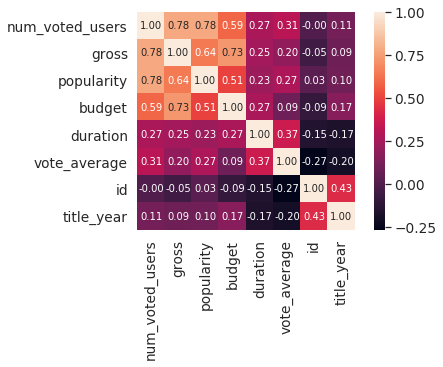
\includegraphics[width=10cm]{./contenido/imagenes/output_80_0.png}

\end{figure}
    { \hspace*{\fill} \\}
    
    Se usará este hallazgo para completar los valores faltantes de las
variables \textbf{gross} y \textbf{num\_voted\_users}. Para ello, se
realizarán regresiones en parejas de variables correlacionadas:

    \begin{tcolorbox}[breakable, size=fbox, boxrule=1pt, pad at break*=1mm,colback=cellbackground, colframe=cellborder]
\prompt{In}{incolor}{53}{\hspace{4pt}}
\begin{Verbatim}[commandchars=\\\{\}]
\PY{n}{sns}\PY{o}{.}\PY{n}{set}\PY{p}{(}\PY{n}{font\PYZus{}scale}\PY{o}{=}\PY{l+m+mf}{1.25}\PY{p}{)}
\PY{c+c1}{\PYZsh{}cols = [\PYZsq{}gross\PYZsq{}, \PYZsq{}num\PYZus{}voted\PYZus{}users\PYZsq{}, \PYZsq{}num\PYZus{}critic\PYZus{}for\PYZus{}reviews\PYZsq{}, \PYZsq{}num\PYZus{}user\PYZus{}for\PYZus{}reviews\PYZsq{}]}
\PY{n}{cols} \PY{o}{=} \PY{p}{[}\PY{l+s+s1}{\PYZsq{}}\PY{l+s+s1}{gross}\PY{l+s+s1}{\PYZsq{}}\PY{p}{,} \PY{l+s+s1}{\PYZsq{}}\PY{l+s+s1}{num\PYZus{}voted\PYZus{}users}\PY{l+s+s1}{\PYZsq{}}\PY{p}{]}
\PY{n}{sns}\PY{o}{.}\PY{n}{pairplot}\PY{p}{(}\PY{n}{df\PYZus{}filling}\PY{o}{.}\PY{n}{dropna}\PY{p}{(}\PY{n}{how}\PY{o}{=}\PY{l+s+s1}{\PYZsq{}}\PY{l+s+s1}{any}\PY{l+s+s1}{\PYZsq{}}\PY{p}{)}\PY{p}{[}\PY{n}{cols}\PY{p}{]}\PY{p}{,}\PY{n}{diag\PYZus{}kind}\PY{o}{=}\PY{l+s+s1}{\PYZsq{}}\PY{l+s+s1}{kde}\PY{l+s+s1}{\PYZsq{}}\PY{p}{,} \PY{n}{size} \PY{o}{=} \PY{l+m+mf}{2.5}\PY{p}{)}
\PY{n}{plt}\PY{o}{.}\PY{n}{show}\PY{p}{(}\PY{p}{)}\PY{p}{;}
\end{Verbatim}
\end{tcolorbox}

\begin{figure}[h]
    \centering
    \captionsetup{width=10cm}
    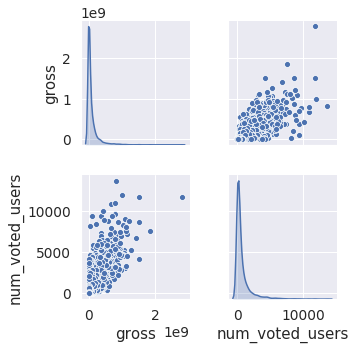
\includegraphics[width=10cm]{./contenido/imagenes/output_82_0.png}

\end{figure}
    { \hspace*{\fill} \\}
    
    En primer lugar, definimos una función que imputa los vbalores faltantes
mediante un ajuste lineal de los datos:

    \begin{tcolorbox}[breakable, size=fbox, boxrule=1pt, pad at break*=1mm,colback=cellbackground, colframe=cellborder]
\prompt{In}{incolor}{54}{\hspace{4pt}}
\begin{Verbatim}[commandchars=\\\{\}]
\PY{k}{def} \PY{n+nf}{regression\PYZus{}imputation}\PY{p}{(}\PY{n}{df}\PY{p}{,} \PY{n}{col\PYZus{}to\PYZus{}predict}\PY{p}{,} \PY{n}{ref\PYZus{}col}\PY{p}{)}\PY{p}{:}
    \PY{l+s+sd}{\PYZdq{}\PYZdq{}\PYZdq{}Completa los valores de la variable col\PYZus{}to\PYZus{}predict haciendo una regresión}
\PY{l+s+sd}{    lineal en la que la variable predictora es ref\PYZus{}col.}

\PY{l+s+sd}{    Args:}
\PY{l+s+sd}{        df (pd.DataFrame): DataFrame de películas}
\PY{l+s+sd}{        col\PYZus{}to\PYZus{}predict (str): Variable a predecir}
\PY{l+s+sd}{        ref\PYZus{}col (str): Variable con la que predecir}

\PY{l+s+sd}{    Returns:}
\PY{l+s+sd}{        pd.DataFrame: DataFrame de películas completado}
\PY{l+s+sd}{    \PYZdq{}\PYZdq{}\PYZdq{}}
    \PY{n}{regr} \PY{o}{=} \PY{n}{linear\PYZus{}model}\PY{o}{.}\PY{n}{LinearRegression}\PY{p}{(}\PY{p}{)}
    \PY{n}{test} \PY{o}{=} \PY{n}{df}\PY{p}{[}\PY{p}{[}\PY{n}{col\PYZus{}to\PYZus{}predict}\PY{p}{,}\PY{n}{ref\PYZus{}col}\PY{p}{]}\PY{p}{]}\PY{o}{.}\PY{n}{dropna}\PY{p}{(}\PY{n}{how}\PY{o}{=}\PY{l+s+s1}{\PYZsq{}}\PY{l+s+s1}{any}\PY{l+s+s1}{\PYZsq{}}\PY{p}{,} \PY{n}{axis} \PY{o}{=} \PY{l+m+mi}{0}\PY{p}{)}
    \PY{n}{X} \PY{o}{=} \PY{n}{np}\PY{o}{.}\PY{n}{array}\PY{p}{(}\PY{n}{test}\PY{p}{[}\PY{n}{ref\PYZus{}col}\PY{p}{]}\PY{p}{)}
    \PY{n}{Y} \PY{o}{=} \PY{n}{np}\PY{o}{.}\PY{n}{array}\PY{p}{(}\PY{n}{test}\PY{p}{[}\PY{n}{col\PYZus{}to\PYZus{}predict}\PY{p}{]}\PY{p}{)}
    \PY{n}{X} \PY{o}{=} \PY{n}{X}\PY{o}{.}\PY{n}{reshape}\PY{p}{(}\PY{n+nb}{len}\PY{p}{(}\PY{n}{X}\PY{p}{)}\PY{p}{,}\PY{l+m+mi}{1}\PY{p}{)}
    \PY{n}{Y} \PY{o}{=} \PY{n}{Y}\PY{o}{.}\PY{n}{reshape}\PY{p}{(}\PY{n+nb}{len}\PY{p}{(}\PY{n}{Y}\PY{p}{)}\PY{p}{,}\PY{l+m+mi}{1}\PY{p}{)}
    \PY{n}{regr}\PY{o}{.}\PY{n}{fit}\PY{p}{(}\PY{n}{X}\PY{p}{,} \PY{n}{Y}\PY{p}{)}

    \PY{n}{test} \PY{o}{=} \PY{n}{df}\PY{p}{[}\PY{n}{df}\PY{p}{[}\PY{n}{col\PYZus{}to\PYZus{}predict}\PY{p}{]}\PY{o}{.}\PY{n}{isnull}\PY{p}{(}\PY{p}{)} \PY{o}{\PYZam{}} \PY{n}{df}\PY{p}{[}\PY{n}{ref\PYZus{}col}\PY{p}{]}\PY{o}{.}\PY{n}{notnull}\PY{p}{(}\PY{p}{)}\PY{p}{]}
    \PY{k}{for} \PY{n}{index}\PY{p}{,} \PY{n}{row} \PY{o+ow}{in} \PY{n}{test}\PY{o}{.}\PY{n}{iterrows}\PY{p}{(}\PY{p}{)}\PY{p}{:}
        \PY{n}{value} \PY{o}{=} \PY{n+nb}{float}\PY{p}{(}\PY{n}{regr}\PY{o}{.}\PY{n}{predict}\PY{p}{(}\PY{n}{row}\PY{p}{[}\PY{n}{ref\PYZus{}col}\PY{p}{]}\PY{p}{)}\PY{p}{)}
        \PY{n}{df}\PY{o}{.}\PY{n}{at}\PY{p}{[}\PY{n}{index}\PY{p}{,} \PY{n}{col\PYZus{}to\PYZus{}predict}\PY{p}{]} \PY{o}{=}  \PY{n}{value}
    \PY{k}{return} \PY{n}{df}
\end{Verbatim}
\end{tcolorbox}

    Esta función toma el dataframe como entrada y los nombres de dos
columnas. Se realiza un ajuste lineal entre estas dos columnas y se usa
para rellenar los datos faltantes de la primera columna dada:

    \begin{tcolorbox}[breakable, size=fbox, boxrule=1pt, pad at break*=1mm,colback=cellbackground, colframe=cellborder]
\prompt{In}{incolor}{55}{\hspace{4pt}}
\begin{Verbatim}[commandchars=\\\{\}]
\PY{n}{df\PYZus{}filling} \PY{o}{=} \PY{n}{regression\PYZus{}imputation}\PY{p}{(}\PY{n}{df\PYZus{}filling}\PY{p}{,} \PY{l+s+s1}{\PYZsq{}}\PY{l+s+s1}{gross}\PY{l+s+s1}{\PYZsq{}}\PY{p}{,} \PY{l+s+s1}{\PYZsq{}}\PY{l+s+s1}{num\PYZus{}voted\PYZus{}users}\PY{l+s+s1}{\PYZsq{}}\PY{p}{)}
\end{Verbatim}
\end{tcolorbox}

    Por último, puede verse a cantidad de información faltante aun en el
dataframe:

    \begin{tcolorbox}[breakable, size=fbox, boxrule=1pt, pad at break*=1mm,colback=cellbackground, colframe=cellborder]
\prompt{In}{incolor}{56}{\hspace{4pt}}
\begin{Verbatim}[commandchars=\\\{\}]
\PY{n}{df} \PY{o}{=} \PY{n}{df\PYZus{}filling}\PY{o}{.}\PY{n}{copy}\PY{p}{(}\PY{n}{deep} \PY{o}{=} \PY{k+kc}{True}\PY{p}{)}
\PY{n}{missing\PYZus{}df} \PY{o}{=} \PY{n}{df}\PY{o}{.}\PY{n}{isnull}\PY{p}{(}\PY{p}{)}\PY{o}{.}\PY{n}{sum}\PY{p}{(}\PY{n}{axis}\PY{o}{=}\PY{l+m+mi}{0}\PY{p}{)}\PY{o}{.}\PY{n}{reset\PYZus{}index}\PY{p}{(}\PY{p}{)}
\PY{n}{missing\PYZus{}df}\PY{o}{.}\PY{n}{columns} \PY{o}{=} \PY{p}{[}\PY{l+s+s1}{\PYZsq{}}\PY{l+s+s1}{column\PYZus{}name}\PY{l+s+s1}{\PYZsq{}}\PY{p}{,} \PY{l+s+s1}{\PYZsq{}}\PY{l+s+s1}{missing\PYZus{}count}\PY{l+s+s1}{\PYZsq{}}\PY{p}{]}
\PY{n}{missing\PYZus{}df}\PY{p}{[}\PY{l+s+s1}{\PYZsq{}}\PY{l+s+s1}{filling\PYZus{}factor}\PY{l+s+s1}{\PYZsq{}}\PY{p}{]} \PY{o}{=} \PY{p}{(}\PY{n}{df}\PY{o}{.}\PY{n}{shape}\PY{p}{[}\PY{l+m+mi}{0}\PY{p}{]} 
                                \PY{o}{\PYZhy{}} \PY{n}{missing\PYZus{}df}\PY{p}{[}\PY{l+s+s1}{\PYZsq{}}\PY{l+s+s1}{missing\PYZus{}count}\PY{l+s+s1}{\PYZsq{}}\PY{p}{]}\PY{p}{)} \PY{o}{/} \PY{n}{df}\PY{o}{.}\PY{n}{shape}\PY{p}{[}\PY{l+m+mi}{0}\PY{p}{]} \PY{o}{*} \PY{l+m+mi}{100}
\PY{n}{missing\PYZus{}df} \PY{o}{=} \PY{n}{missing\PYZus{}df}\PY{o}{.}\PY{n}{sort\PYZus{}values}\PY{p}{(}\PY{l+s+s1}{\PYZsq{}}\PY{l+s+s1}{filling\PYZus{}factor}\PY{l+s+s1}{\PYZsq{}}\PY{p}{)}\PY{o}{.}\PY{n}{reset\PYZus{}index}\PY{p}{(}\PY{n}{drop} \PY{o}{=} \PY{k+kc}{True}\PY{p}{)}
\PY{n}{missing\PYZus{}df}
\end{Verbatim}
\end{tcolorbox}

            \begin{tcolorbox}[breakable, boxrule=.5pt, size=fbox, pad at break*=1mm, opacityfill=0]
\prompt{Out}{outcolor}{56}{\hspace{3.5pt}}
\begin{Verbatim}[commandchars=\\\{\}]
        column\_name  missing\_count  filling\_factor
0           country            174       96.377264
1      actor\_3\_name             93       98.063710
2          language             86       98.209452
3      actor\_2\_name             63       98.688320
4      actor\_1\_name             53       98.896523
5     director\_name             30       99.375390
6          duration              2       99.958359
7        title\_year              1       99.979180
8       movie\_title              0      100.000000
9            genres              0      100.000000
10    plot\_keywords              0      100.000000
11  num\_voted\_users              0      100.000000
12     vote\_average              0      100.000000
13            gross              0      100.000000
\end{Verbatim}
\end{tcolorbox}
        
    y puede verse que en el peor de los casos el la completitud está
alrededor del 96\%.

    \begin{tcolorbox}[breakable, size=fbox, boxrule=1pt, pad at break*=1mm,colback=cellbackground, colframe=cellborder]
\prompt{In}{incolor}{57}{\hspace{4pt}}
\begin{Verbatim}[commandchars=\\\{\}]
\PY{n}{df} \PY{o}{=} \PY{n}{df\PYZus{}filling}\PY{o}{.}\PY{n}{copy}\PY{p}{(}\PY{n}{deep}\PY{o}{=}\PY{k+kc}{True}\PY{p}{)}
\PY{n}{df}\PY{o}{.}\PY{n}{reset\PYZus{}index}\PY{p}{(}\PY{n}{inplace} \PY{o}{=} \PY{k+kc}{True}\PY{p}{,} \PY{n}{drop} \PY{o}{=} \PY{k+kc}{True}\PY{p}{)}
\end{Verbatim}
\end{tcolorbox}

    \begin{center}\rule{0.5\linewidth}{\linethickness}\end{center}

\subsection{3. MOTOR DE RECOMENDACIÓN}\label{motor-de-recomendaciuxf3n}

    \begin{center}\rule{0.5\linewidth}{\linethickness}\end{center}

\subsubsection{3.1 Funcionamiento básico del
motor}\label{funcionamiento-buxe1sico-del-motor}

El orden para construir el motor de recomendación tendrá dos pasos
básicos: 1. Elegir \(N\) películas con un contenido similar a la entrada
dada por el usuario 2. Seleccionar las 5 películas mas populares de
entre esas \(N\) películas

\paragraph{3.1.1 Similaridad}\label{similaridad}

Cuando se construye el motor, el primer paso consiste en definir un
criterio que pueda aportar información sobre cómo de parecidas son dos
películas. En primer lugar, tenemos en cuenta la descripción de la
película seleccionada por el usuario. De ahi tomamos el director, los
nombres de los actores y algunas keywords. A partir de estos datos,
creamos una matriz en la que cada fila se corresponde con una película
de la base de datos y en la que las columnas corresponden con lo dicho
anteriormente junto con los \emph{k} generos que se describieron en la
sección 1.4:

    \begin{table}[]
\centering
\begin{tabular}{|l|l|l|l|l|l|l|l|l|l|l|}
\hline
\textbf{\begin{tabular}[c]{@{}l@{}}movie\\ title\end{tabular}} &
  \textbf{director} &
  \textbf{actor 1} &
  \textbf{a2} &
  \textbf{a3} &
  \textbf{keyword 1} &
  \textbf{k2} &
  \textbf{genre1} &
  \textbf{g2} &
  \textbf{...} &
  \textbf{gk} \\ \hline
Film1  & $a_{11}$ & $a_{12}$ &  &  & ...      &  &  &  & ... & $a_{1q}$ \\ \hline
...    &          &          &  &  & ...      &  &  &  & ... &          \\ \hline
Film i & $a_{i1}$ & $a_{i2}$ &  &  & $a_{ij}$ &  &  &  & ... & $a_{iq}$ \\ \hline
...    &          &          &  &  & ...      &  &  &  & ... &          \\ \hline
Film p & $a_{p1}$ & $a_{p2}$ &  &  & ...      &  &  &  & ... & $a_{pq}$ \\ \hline
\end{tabular}
\caption{Matriz generada para el cálculo de la similaridad entre dos películas}
\label{tab:similarity}
\end{table}

    En esta matriz, el elemento \(a_{ij}\) toma el valor 0 o 1 dependiendo
de la correspondencia entre la significancia entre la columna \(j\) y el
contenido de la película \(i\). Por ejemplo, si "keyword1" está en la
película \(i\), tendremos \(a_{ij} = 1\) y \(0\) en otro caso. Una vez
esta matriz se ha definido, determinamos la distnaica entre dos
películas mediante:

\begin{eqnarray}
d_{m, n} = \sqrt{  \sum_{i = 1}^{N} \left( a_{m,i}  - a_{n,i} \right)^2  } 
\end{eqnarray}

En este punto, únicamente tenemos que seleccionar las \(N\) películas
que son más cercanas a la entrada seleccionada por el usuario.

\paragraph{3.1.2 Popularidad}\label{popularidad}

Atendiendo a la similaridad entre películas, seleccionamos una lista de
\(N\) películas. En etse punto, seleccionaremos únicamente 5 películas.
Para ello, damos una puntuación a cada entrada. Se computa la puntuación
de acuerdo a estos tres criterios: - La puntuación en IMDB - El número
de votos recibidos por la película - El año de lanzamiento

Los dos primeros serán una medida directa de la popularidad de varias
entradas. Para el tercer criterio, se introduce el año de lanzamiento.
Se asume que las preferidas por la persona serán en la mayoria de los
casos de la misma época.

A continuación, calculamos la puntuación de acuerdo a esta ecuación:

    \begin{eqnarray}
\mathrm{score} = IMDB^2 \times \phi_{\sigma_1, c_1} \times  \phi_{\sigma_2, c_2},
\end{eqnarray}

donde \(\phi\) es una función gaussiana del tipo

\begin{eqnarray}
\phi_{\sigma, c}(x) \propto \mathrm{exp}\left(-\frac{(x-c)^2}{2 \, \sigma^2}\right).
\end{eqnarray}

    Para lo votos, tomamos el máximo número de votos entre las \(N\)
películas y fijamos \(\sigma_1 = c_1 = m\). Para lso años, ponemos
\(\sigma_1 = 20\) y centramos la gaussiana en el año de la película
seleccionada por el usuario. Con las gaussianas, se pone más peso en las
entradas con mayor número de votos y en las que el año de salida es
cercano al de la película seleccionada por el usuario.

    \begin{tcolorbox}[breakable, size=fbox, boxrule=1pt, pad at break*=1mm,colback=cellbackground, colframe=cellborder]
\prompt{In}{incolor}{58}{\hspace{4pt}}
\begin{Verbatim}[commandchars=\\\{\}]
\PY{n}{df}
\end{Verbatim}
\end{tcolorbox}

            \begin{tcolorbox}[breakable, boxrule=.5pt, size=fbox, pad at break*=1mm, opacityfill=0]
\prompt{Out}{outcolor}{58}{\hspace{3.5pt}}
\begin{Verbatim}[commandchars=\\\{\}]
                                   movie\_title  title\_year  \textbackslash{}
0                                       Avatar      2009.0
1     Pirates of the Caribbean: At World's End      2007.0
2                                      Spectre      2015.0
3                        The Dark Knight Rises      2012.0
4                                  John Carter      2012.0
{\ldots}                                        {\ldots}         {\ldots}
4798                               El Mariachi      1992.0
4799                                 Newlyweds      2011.0
4800                 Signed, Sealed, Delivered      2013.0
4801                          Shanghai Calling      2012.0
4802                         My Date with Drew      2005.0

                                        genres  \textbackslash{}
0     Action|Adventure|Fantasy|Science Fiction
1                     Adventure|Fantasy|Action
2                       Action|Adventure|Crime
3                  Action|Crime|Drama|Thriller
4             Action|Adventure|Science Fiction
{\ldots}                                        {\ldots}
4798                     Action|Crime|Thriller
4799                            Comedy|Romance
4800             Comedy|Drama|Romance|TV Movie
4801
4802                               Documentary

                                          plot\_keywords      director\_name  \textbackslash{}
0     culture clash|future|space colony|society|spac{\ldots}      James Cameron
1     ocean|drug abuse|exotic island|east india trad{\ldots}     Gore Verbinski
2     spy|based on novel|secret agent|sequel|british{\ldots}         Sam Mendes
3     dc comics|crime fighter|terrorist|secret ident{\ldots}  Christopher Nolan
4     based on novel|mars|medallion|space travel|pri{\ldots}     Andrew Stanton
{\ldots}                                                 {\ldots}                {\ldots}
4798     united states–mexico barrier|stagecoach|weapon   Robert Rodriguez
4799                                                          Edward Burns
4800  date|love at first sight|narration|investigato{\ldots}        Scott Smith
4801                                                           Daniel Hsia
4802                          obsession|camcorder|crush   Brian Herzlinger

          actor\_1\_name      actor\_2\_name        actor\_3\_name  num\_voted\_users  \textbackslash{}
0          Zoe Saldana  Sigourney Weaver        Stephen Lang            11800
1        Orlando Bloom   Keira Knightley   Stellan Skarsgård             4500
2      Christoph Waltz       Léa Seydoux       Ralph Fiennes             4466
3        Michael Caine       Gary Oldman       Anne Hathaway             9106
4         Lynn Collins   Samantha Morton        Willem Dafoe             2124
{\ldots}                {\ldots}               {\ldots}                 {\ldots}              {\ldots}
4798    Jaime de Hoyos   Peter Marquardt     Reinol Martinez              238
4799       Kerry Bishé   Marsha Dietlein  Caitlin Fitzgerald                5
4800     Kristin Booth      Crystal Lowe     Geoff Gustafson                6
4801       Eliza Coupe       Bill Paxton           Alan Ruck                7
4802  Brian Herzlinger     Corey Feldman        Eric Roberts               16

      language                   country  vote\_average  duration       gross
0      English  United States of America           7.2     162.0  2787965087
1      English  United States of America           6.9     169.0   961000000
2     Français            United Kingdom           6.3     148.0   880674609
3      English  United States of America           7.6     165.0  1084939099
4      English  United States of America           6.1     132.0   284139100
{\ldots}        {\ldots}                       {\ldots}           {\ldots}       {\ldots}         {\ldots}
4798   Español                    Mexico           6.6      81.0     2040920
4799       NaN                       NaN           5.9      85.0           0
4800   English  United States of America           7.0     120.0           0
4801   English  United States of America           5.7      98.0           0
4802   English  United States of America           6.3      90.0           0

[4803 rows x 14 columns]
\end{Verbatim}
\end{tcolorbox}
        
    \begin{center}\rule{0.5\linewidth}{\linethickness}\end{center}

\subsubsection{3.2 Definición de las funciones del
motor}\label{definiciuxf3n-de-las-funciones-del-motor}

    \begin{tcolorbox}[breakable, size=fbox, boxrule=1pt, pad at break*=1mm,colback=cellbackground, colframe=cellborder]
\prompt{In}{incolor}{80}{\hspace{4pt}}
\begin{Verbatim}[commandchars=\\\{\}]
\PY{n}{gaussian\PYZus{}filter} \PY{o}{=} \PY{k}{lambda} \PY{n}{x}\PY{p}{,}\PY{n}{y}\PY{p}{,}\PY{n}{sigma}\PY{p}{:} \PY{n}{math}\PY{o}{.}\PY{n}{exp}\PY{p}{(}\PY{o}{\PYZhy{}}\PY{p}{(}\PY{n}{x}\PY{o}{\PYZhy{}}\PY{n}{y}\PY{p}{)}\PY{o}{*}\PY{o}{*}\PY{l+m+mi}{2}\PY{o}{/}\PY{p}{(}\PY{l+m+mi}{2}\PY{o}{*}\PY{n}{sigma}\PY{o}{*}\PY{o}{*}\PY{l+m+mi}{2}\PY{p}{)}\PY{p}{)}
\end{Verbatim}
\end{tcolorbox}

    \begin{tcolorbox}[breakable, size=fbox, boxrule=1pt, pad at break*=1mm,colback=cellbackground, colframe=cellborder]
\prompt{In}{incolor}{81}{\hspace{4pt}}
\begin{Verbatim}[commandchars=\\\{\}]
\PY{k}{def} \PY{n+nf}{entry\PYZus{}variables}\PY{p}{(}\PY{n}{df}\PY{p}{,} \PY{n}{id\PYZus{}entry}\PY{p}{)}\PY{p}{:} 
    \PY{l+s+sd}{\PYZdq{}\PYZdq{}\PYZdq{}Calcula los valores tomados por las variables director\PYZus{}name, actor\PYZus{}[1,2,3]\PYZus{}name y plot\PYZus{}keywords para la}
\PY{l+s+sd}{    película seleccionada por el usuario.}

\PY{l+s+sd}{    Args:}
\PY{l+s+sd}{        df (pd.DataFrame): DataFrame de películas}
\PY{l+s+sd}{        id\PYZus{}entry (int): Id de la entrada seleccionada}

\PY{l+s+sd}{    Returns:}
\PY{l+s+sd}{        list: Lista que contiene los valores extraidos para la película seleccionada}
\PY{l+s+sd}{    \PYZdq{}\PYZdq{}\PYZdq{}}
    
    \PY{n}{col\PYZus{}labels} \PY{o}{=} \PY{p}{[}\PY{p}{]}    
    \PY{k}{if} \PY{n}{pd}\PY{o}{.}\PY{n}{notnull}\PY{p}{(}\PY{n}{df}\PY{p}{[}\PY{l+s+s1}{\PYZsq{}}\PY{l+s+s1}{director\PYZus{}name}\PY{l+s+s1}{\PYZsq{}}\PY{p}{]}\PY{o}{.}\PY{n}{iloc}\PY{p}{[}\PY{n}{id\PYZus{}entry}\PY{p}{]}\PY{p}{)}\PY{p}{:}
        \PY{k}{for} \PY{n}{s} \PY{o+ow}{in} \PY{n}{df}\PY{p}{[}\PY{l+s+s1}{\PYZsq{}}\PY{l+s+s1}{director\PYZus{}name}\PY{l+s+s1}{\PYZsq{}}\PY{p}{]}\PY{o}{.}\PY{n}{iloc}\PY{p}{[}\PY{n}{id\PYZus{}entry}\PY{p}{]}\PY{o}{.}\PY{n}{split}\PY{p}{(}\PY{l+s+s1}{\PYZsq{}}\PY{l+s+s1}{|}\PY{l+s+s1}{\PYZsq{}}\PY{p}{)}\PY{p}{:}
            \PY{n}{col\PYZus{}labels}\PY{o}{.}\PY{n}{append}\PY{p}{(}\PY{n}{s}\PY{p}{)}
            
    \PY{k}{for} \PY{n}{i} \PY{o+ow}{in} \PY{n+nb}{range}\PY{p}{(}\PY{l+m+mi}{3}\PY{p}{)}\PY{p}{:}
        \PY{n}{column} \PY{o}{=} \PY{l+s+s1}{\PYZsq{}}\PY{l+s+s1}{actor\PYZus{}NUM\PYZus{}name}\PY{l+s+s1}{\PYZsq{}}\PY{o}{.}\PY{n}{replace}\PY{p}{(}\PY{l+s+s1}{\PYZsq{}}\PY{l+s+s1}{NUM}\PY{l+s+s1}{\PYZsq{}}\PY{p}{,} \PY{n+nb}{str}\PY{p}{(}\PY{n}{i}\PY{o}{+}\PY{l+m+mi}{1}\PY{p}{)}\PY{p}{)}
        \PY{k}{if} \PY{n}{pd}\PY{o}{.}\PY{n}{notnull}\PY{p}{(}\PY{n}{df}\PY{p}{[}\PY{n}{column}\PY{p}{]}\PY{o}{.}\PY{n}{iloc}\PY{p}{[}\PY{n}{id\PYZus{}entry}\PY{p}{]}\PY{p}{)}\PY{p}{:}
            \PY{k}{for} \PY{n}{s} \PY{o+ow}{in} \PY{n}{df}\PY{p}{[}\PY{n}{column}\PY{p}{]}\PY{o}{.}\PY{n}{iloc}\PY{p}{[}\PY{n}{id\PYZus{}entry}\PY{p}{]}\PY{o}{.}\PY{n}{split}\PY{p}{(}\PY{l+s+s1}{\PYZsq{}}\PY{l+s+s1}{|}\PY{l+s+s1}{\PYZsq{}}\PY{p}{)}\PY{p}{:}
                \PY{n}{col\PYZus{}labels}\PY{o}{.}\PY{n}{append}\PY{p}{(}\PY{n}{s}\PY{p}{)}
                
    \PY{k}{if} \PY{n}{pd}\PY{o}{.}\PY{n}{notnull}\PY{p}{(}\PY{n}{df}\PY{p}{[}\PY{l+s+s1}{\PYZsq{}}\PY{l+s+s1}{plot\PYZus{}keywords}\PY{l+s+s1}{\PYZsq{}}\PY{p}{]}\PY{o}{.}\PY{n}{iloc}\PY{p}{[}\PY{n}{id\PYZus{}entry}\PY{p}{]}\PY{p}{)}\PY{p}{:}
        \PY{k}{for} \PY{n}{s} \PY{o+ow}{in} \PY{n}{df}\PY{p}{[}\PY{l+s+s1}{\PYZsq{}}\PY{l+s+s1}{plot\PYZus{}keywords}\PY{l+s+s1}{\PYZsq{}}\PY{p}{]}\PY{o}{.}\PY{n}{iloc}\PY{p}{[}\PY{n}{id\PYZus{}entry}\PY{p}{]}\PY{o}{.}\PY{n}{split}\PY{p}{(}\PY{l+s+s1}{\PYZsq{}}\PY{l+s+s1}{|}\PY{l+s+s1}{\PYZsq{}}\PY{p}{)}\PY{p}{:}
            \PY{n}{col\PYZus{}labels}\PY{o}{.}\PY{n}{append}\PY{p}{(}\PY{n}{s}\PY{p}{)}
    \PY{k}{return} \PY{n}{col\PYZus{}labels}
\end{Verbatim}
\end{tcolorbox}

    \begin{tcolorbox}[breakable, size=fbox, boxrule=1pt, pad at break*=1mm,colback=cellbackground, colframe=cellborder]
\prompt{In}{incolor}{82}{\hspace{4pt}}
\begin{Verbatim}[commandchars=\\\{\}]
\PY{n}{df}\PY{o}{.}\PY{n}{head}\PY{p}{(}\PY{l+m+mi}{2}\PY{p}{)}
\end{Verbatim}
\end{tcolorbox}

            \begin{tcolorbox}[breakable, boxrule=.5pt, size=fbox, pad at break*=1mm, opacityfill=0]
\prompt{Out}{outcolor}{82}{\hspace{3.5pt}}
\begin{Verbatim}[commandchars=\\\{\}]
                                movie\_title  title\_year  \textbackslash{}
0                                    Avatar      2009.0
1  Pirates of the Caribbean: At World's End      2007.0

                                     genres  \textbackslash{}
0  Action|Adventure|Fantasy|Science Fiction
1                  Adventure|Fantasy|Action

                                       plot\_keywords   director\_name  \textbackslash{}
0  culture clash|future|space colony|society|spac{\ldots}   James Cameron
1  ocean|drug abuse|exotic island|east india trad{\ldots}  Gore Verbinski

    actor\_1\_name      actor\_2\_name       actor\_3\_name  num\_voted\_users  \textbackslash{}
0    Zoe Saldana  Sigourney Weaver       Stephen Lang            11800
1  Orlando Bloom   Keira Knightley  Stellan Skarsgård             4500

  language                   country  vote\_average  duration       gross
0  English  United States of America           7.2     162.0  2787965087
1  English  United States of America           6.9     169.0   961000000
\end{Verbatim}
\end{tcolorbox}
        
    \begin{tcolorbox}[breakable, size=fbox, boxrule=1pt, pad at break*=1mm,colback=cellbackground, colframe=cellborder]
\prompt{In}{incolor}{83}{\hspace{4pt}}
\begin{Verbatim}[commandchars=\\\{\}]
\PY{k}{def} \PY{n+nf}{add\PYZus{}variables}\PY{p}{(}\PY{n}{df}\PY{p}{,} \PY{n}{REF\PYZus{}VAR}\PY{p}{)}\PY{p}{:}
    \PY{l+s+sd}{\PYZdq{}\PYZdq{}\PYZdq{}Añade al dataframe de películas las columnas dadas en REF\PYZus{}VAR (que serán el }
\PY{l+s+sd}{    director, etc de unapelícula) y las inicializa a 0 o 1 dependiendo de si la }
\PY{l+s+sd}{    película es del mismo director, tiene a ese actor, etc}

\PY{l+s+sd}{    Args:}
\PY{l+s+sd}{        df (pd.DataFrame): DataFrame de películas}
\PY{l+s+sd}{        REF\PYZus{}VAR (list): Salida de aplicar entry\PYZus{}variables sobre el df y una película}

\PY{l+s+sd}{    Returns:}
\PY{l+s+sd}{        pd.DataFrame: DataFrame con las nuevas películas}
\PY{l+s+sd}{    \PYZdq{}\PYZdq{}\PYZdq{}}
    \PY{k}{for} \PY{n}{s} \PY{o+ow}{in} \PY{n}{REF\PYZus{}VAR}\PY{p}{:} 
        \PY{n}{df}\PY{p}{[}\PY{n}{s}\PY{p}{]} \PY{o}{=} \PY{n}{pd}\PY{o}{.}\PY{n}{Series}\PY{p}{(}\PY{p}{[}\PY{l+m+mi}{0} \PY{k}{for} \PY{n}{\PYZus{}} \PY{o+ow}{in} \PY{n+nb}{range}\PY{p}{(}\PY{n+nb}{len}\PY{p}{(}\PY{n}{df}\PY{p}{)}\PY{p}{)}\PY{p}{]}\PY{p}{)}
    \PY{n}{columns} \PY{o}{=} \PY{p}{[}\PY{l+s+s1}{\PYZsq{}}\PY{l+s+s1}{genres}\PY{l+s+s1}{\PYZsq{}}\PY{p}{,} \PY{l+s+s1}{\PYZsq{}}\PY{l+s+s1}{actor\PYZus{}1\PYZus{}name}\PY{l+s+s1}{\PYZsq{}}\PY{p}{,} \PY{l+s+s1}{\PYZsq{}}\PY{l+s+s1}{actor\PYZus{}2\PYZus{}name}\PY{l+s+s1}{\PYZsq{}}\PY{p}{,}
                \PY{l+s+s1}{\PYZsq{}}\PY{l+s+s1}{actor\PYZus{}3\PYZus{}name}\PY{l+s+s1}{\PYZsq{}}\PY{p}{,} \PY{l+s+s1}{\PYZsq{}}\PY{l+s+s1}{director\PYZus{}name}\PY{l+s+s1}{\PYZsq{}}\PY{p}{,} \PY{l+s+s1}{\PYZsq{}}\PY{l+s+s1}{plot\PYZus{}keywords}\PY{l+s+s1}{\PYZsq{}}\PY{p}{]}
    \PY{k}{for} \PY{n}{category} \PY{o+ow}{in} \PY{n}{columns}\PY{p}{:}
        \PY{k}{for} \PY{n}{index}\PY{p}{,} \PY{n}{row} \PY{o+ow}{in} \PY{n}{df}\PY{o}{.}\PY{n}{iterrows}\PY{p}{(}\PY{p}{)}\PY{p}{:}
            \PY{k}{if} \PY{n}{pd}\PY{o}{.}\PY{n}{isnull}\PY{p}{(}\PY{n}{row}\PY{p}{[}\PY{n}{category}\PY{p}{]}\PY{p}{)}\PY{p}{:} 
                \PY{k}{continue}
            \PY{k}{for} \PY{n}{s} \PY{o+ow}{in} \PY{n}{row}\PY{p}{[}\PY{n}{category}\PY{p}{]}\PY{o}{.}\PY{n}{split}\PY{p}{(}\PY{l+s+s1}{\PYZsq{}}\PY{l+s+s1}{|}\PY{l+s+s1}{\PYZsq{}}\PY{p}{)}\PY{p}{:}
                \PY{k}{if} \PY{n}{s} \PY{o+ow}{in} \PY{n}{REF\PYZus{}VAR}\PY{p}{:} \PY{n}{df}\PY{o}{.}\PY{n}{set\PYZus{}value}\PY{p}{(}\PY{n}{index}\PY{p}{,} \PY{n}{s}\PY{p}{,} \PY{l+m+mi}{1}\PY{p}{)}            
    \PY{k}{return} \PY{n}{df}
\end{Verbatim}
\end{tcolorbox}

    \textbf{Function creating a list of films}: the \emph{recommand()}
function create a list of N (= 31) films similar to the film selected by
the user.

    \begin{tcolorbox}[breakable, size=fbox, boxrule=1pt, pad at break*=1mm,colback=cellbackground, colframe=cellborder]
\prompt{In}{incolor}{84}{\hspace{4pt}}
\begin{Verbatim}[commandchars=\\\{\}]
\PY{k}{def} \PY{n+nf}{recommend}\PY{p}{(}\PY{n}{df}\PY{p}{,} \PY{n}{id\PYZus{}entry}\PY{p}{,} \PY{n}{N} \PY{o}{=} \PY{l+m+mi}{31}\PY{p}{)}\PY{p}{:}
    \PY{l+s+sd}{\PYZdq{}\PYZdq{}\PYZdq{}Crea una lista de N películas similares a las seleccionadas por el usuario}

\PY{l+s+sd}{    Args:}
\PY{l+s+sd}{        df (pd.DataFrame): DataFrame de películas}
\PY{l+s+sd}{        id\PYZus{}entry (int): Id de la entrada seleccionada}
\PY{l+s+sd}{        N (int, optional): Number of films recommended }
\PY{l+s+sd}{        (take into account that the nearest will be always itself). Defaults to 31.}

\PY{l+s+sd}{    Returns:}
\PY{l+s+sd}{        list: List of ids of films recommended}
\PY{l+s+sd}{    \PYZdq{}\PYZdq{}\PYZdq{}}
    \PY{n}{df\PYZus{}copy} \PY{o}{=} \PY{n}{df}\PY{o}{.}\PY{n}{copy}\PY{p}{(}\PY{n}{deep} \PY{o}{=} \PY{k+kc}{True}\PY{p}{)}    
    \PY{n}{list\PYZus{}genres} \PY{o}{=} \PY{n+nb}{set}\PY{p}{(}\PY{p}{)}
    \PY{k}{for} \PY{n}{s} \PY{o+ow}{in} \PY{n}{df}\PY{p}{[}\PY{l+s+s1}{\PYZsq{}}\PY{l+s+s1}{genres}\PY{l+s+s1}{\PYZsq{}}\PY{p}{]}\PY{o}{.}\PY{n}{str}\PY{o}{.}\PY{n}{split}\PY{p}{(}\PY{l+s+s1}{\PYZsq{}}\PY{l+s+s1}{|}\PY{l+s+s1}{\PYZsq{}}\PY{p}{)}\PY{o}{.}\PY{n}{values}\PY{p}{:}
        \PY{n}{list\PYZus{}genres} \PY{o}{=} \PY{n}{list\PYZus{}genres}\PY{o}{.}\PY{n}{union}\PY{p}{(}\PY{n+nb}{set}\PY{p}{(}\PY{n}{s}\PY{p}{)}\PY{p}{)}    

    \PY{c+c1}{\PYZsh{} Creación de variables adicionales para comprobar la similaridad}
    \PY{n}{variables} \PY{o}{=} \PY{n}{entry\PYZus{}variables}\PY{p}{(}\PY{n}{df\PYZus{}copy}\PY{p}{,} \PY{n}{id\PYZus{}entry}\PY{p}{)}
    \PY{n}{variables} \PY{o}{+}\PY{o}{=} \PY{n+nb}{list}\PY{p}{(}\PY{n}{list\PYZus{}genres}\PY{p}{)}
    \PY{n}{df\PYZus{}new} \PY{o}{=} \PY{n}{add\PYZus{}variables}\PY{p}{(}\PY{n}{df\PYZus{}copy}\PY{p}{,} \PY{n}{variables}\PY{p}{)}

    \PY{c+c1}{\PYZsh{} Determinación de los vecinos más próximos: la distancia se calcula con las nuevas vairables}
    \PY{n}{X} \PY{o}{=} \PY{n}{df\PYZus{}new}\PY{o}{.}\PY{n}{as\PYZus{}matrix}\PY{p}{(}\PY{n}{variables}\PY{p}{)}
    \PY{n}{nbrs} \PY{o}{=} \PY{n}{NearestNeighbors}\PY{p}{(}\PY{n}{n\PYZus{}neighbors}\PY{o}{=}\PY{n}{N}\PY{p}{,} \PY{n}{algorithm}\PY{o}{=}\PY{l+s+s1}{\PYZsq{}}\PY{l+s+s1}{auto}\PY{l+s+s1}{\PYZsq{}}\PY{p}{,} \PY{n}{metric}\PY{o}{=}\PY{l+s+s1}{\PYZsq{}}\PY{l+s+s1}{euclidean}\PY{l+s+s1}{\PYZsq{}}\PY{p}{)}\PY{o}{.}\PY{n}{fit}\PY{p}{(}\PY{n}{X}\PY{p}{)}

    \PY{n}{distances}\PY{p}{,} \PY{n}{indices} \PY{o}{=} \PY{n}{nbrs}\PY{o}{.}\PY{n}{kneighbors}\PY{p}{(}\PY{n}{X}\PY{p}{)}    
    \PY{n}{xtest} \PY{o}{=} \PY{n}{df\PYZus{}new}\PY{o}{.}\PY{n}{iloc}\PY{p}{[}\PY{n}{id\PYZus{}entry}\PY{p}{]}\PY{o}{.}\PY{n}{as\PYZus{}matrix}\PY{p}{(}\PY{n}{variables}\PY{p}{)}
    \PY{n}{xtest} \PY{o}{=} \PY{n}{xtest}\PY{o}{.}\PY{n}{reshape}\PY{p}{(}\PY{l+m+mi}{1}\PY{p}{,} \PY{o}{\PYZhy{}}\PY{l+m+mi}{1}\PY{p}{)}

    \PY{n}{distances}\PY{p}{,} \PY{n}{indices} \PY{o}{=} \PY{n}{nbrs}\PY{o}{.}\PY{n}{kneighbors}\PY{p}{(}\PY{n}{xtest}\PY{p}{)}

    \PY{k}{return} \PY{n}{indices}\PY{p}{[}\PY{l+m+mi}{0}\PY{p}{]}\PY{p}{[}\PY{p}{:}\PY{p}{]}
    
\end{Verbatim}
\end{tcolorbox}

    \begin{tcolorbox}[breakable, size=fbox, boxrule=1pt, pad at break*=1mm,colback=cellbackground, colframe=cellborder]
\prompt{In}{incolor}{85}{\hspace{4pt}}
\begin{Verbatim}[commandchars=\\\{\}]
\PY{n}{recommend}\PY{p}{(}\PY{n}{df}\PY{p}{,} \PY{l+m+mi}{2}\PY{p}{)}
\end{Verbatim}
\end{tcolorbox}

            \begin{tcolorbox}[breakable, boxrule=.5pt, size=fbox, pad at break*=1mm, opacityfill=0]
\prompt{Out}{outcolor}{85}{\hspace{3.5pt}}
\begin{Verbatim}[commandchars=\\\{\}]
array([   2,   29,   11, 1234, 1740, 1077, 2675,  425,  640,   62, 1100,
        134,  183, 3336,  469, 1343, 4339, 1542, 3494, 2444, 1615, 2433,
       2995, 1720, 1610, 1586, 3799, 1743, 1713, 4071, 1697])
\end{Verbatim}
\end{tcolorbox}
        
    \textbf{Function extracting some parameters from a list of films}: the
\emph{create\_film\_selection()} function extracts some variables of the
dataframe given in input and returns this list for a selection of N
films. This list is ordered according to criteria established in the
\emph{critere\_selection()} function.

    \begin{tcolorbox}[breakable, size=fbox, boxrule=1pt, pad at break*=1mm,colback=cellbackground, colframe=cellborder]
\prompt{In}{incolor}{86}{\hspace{4pt}}
\begin{Verbatim}[commandchars=\\\{\}]
\PY{k}{def} \PY{n+nf}{extract\PYZus{}parameters}\PY{p}{(}\PY{n}{df}\PY{p}{,} \PY{n}{list\PYZus{}films}\PY{p}{,} \PY{n}{N} \PY{o}{=} \PY{l+m+mi}{31}\PY{p}{)}\PY{p}{:}
    \PY{l+s+sd}{\PYZdq{}\PYZdq{}\PYZdq{}Extrae algunas variables del dataframe dado como entrada y devuelve la lista}
\PY{l+s+sd}{    de N películas. Esta lista se ordena de acuerdo al criterio de la función }
\PY{l+s+sd}{    selection\PYZus{}criteria.}

\PY{l+s+sd}{    Args:}
\PY{l+s+sd}{        df ([type]): DataFrame de películas}
\PY{l+s+sd}{        list\PYZus{}films (list): Lista con las n películas recomendadas}
\PY{l+s+sd}{        N (int, optional): Number of films recommended. Defaults to 31.}

\PY{l+s+sd}{    Returns:}
\PY{l+s+sd}{        list: Películas recomendadas}
\PY{l+s+sd}{    \PYZdq{}\PYZdq{}\PYZdq{}}
    \PY{n}{film\PYZus{}parameters} \PY{o}{=} \PY{p}{[}\PY{l+s+s1}{\PYZsq{}}\PY{l+s+s1}{\PYZus{}}\PY{l+s+s1}{\PYZsq{}} \PY{k}{for} \PY{n}{\PYZus{}} \PY{o+ow}{in} \PY{n+nb}{range}\PY{p}{(}\PY{n}{N}\PY{p}{)}\PY{p}{]}
    \PY{n}{i} \PY{o}{=} \PY{l+m+mi}{0}
    \PY{n}{max\PYZus{}users} \PY{o}{=} \PY{o}{\PYZhy{}}\PY{l+m+mi}{1}
    \PY{k}{for} \PY{n}{index} \PY{o+ow}{in} \PY{n}{list\PYZus{}films}\PY{p}{:}
        \PY{n}{film\PYZus{}parameters}\PY{p}{[}\PY{n}{i}\PY{p}{]} \PY{o}{=} \PY{n+nb}{list}\PY{p}{(}\PY{n}{df}\PY{o}{.}\PY{n}{iloc}\PY{p}{[}\PY{n}{index}\PY{p}{]}\PY{p}{[}\PY{p}{[}\PY{l+s+s1}{\PYZsq{}}\PY{l+s+s1}{movie\PYZus{}title}\PY{l+s+s1}{\PYZsq{}}\PY{p}{,} \PY{l+s+s1}{\PYZsq{}}\PY{l+s+s1}{title\PYZus{}year}\PY{l+s+s1}{\PYZsq{}}\PY{p}{,}
                                        \PY{l+s+s1}{\PYZsq{}}\PY{l+s+s1}{vote\PYZus{}average}\PY{l+s+s1}{\PYZsq{}}\PY{p}{,} 
                                        \PY{l+s+s1}{\PYZsq{}}\PY{l+s+s1}{num\PYZus{}voted\PYZus{}users}\PY{l+s+s1}{\PYZsq{}}\PY{p}{,} \PY{l+s+s1}{\PYZsq{}}\PY{l+s+s1}{gross}\PY{l+s+s1}{\PYZsq{}}\PY{p}{]}\PY{p}{]}\PY{p}{)}
        \PY{n}{film\PYZus{}parameters}\PY{p}{[}\PY{n}{i}\PY{p}{]}\PY{o}{.}\PY{n}{append}\PY{p}{(}\PY{n}{index}\PY{p}{)}
        \PY{n}{max\PYZus{}users} \PY{o}{=} \PY{n+nb}{max}\PY{p}{(}\PY{n}{max\PYZus{}users}\PY{p}{,} \PY{n}{film\PYZus{}parameters}\PY{p}{[}\PY{n}{i}\PY{p}{]}\PY{p}{[}\PY{l+m+mi}{4}\PY{p}{]} \PY{p}{)}
        \PY{n}{i} \PY{o}{+}\PY{o}{=} \PY{l+m+mi}{1}
    \PY{c+c1}{\PYZsh{} The first element is the selected film itself}
    \PY{n}{title\PYZus{}main} \PY{o}{=} \PY{n}{film\PYZus{}parameters}\PY{p}{[}\PY{l+m+mi}{0}\PY{p}{]}\PY{p}{[}\PY{l+m+mi}{0}\PY{p}{]}
    \PY{n}{ref\PYZus{}year}  \PY{o}{=} \PY{n}{film\PYZus{}parameters}\PY{p}{[}\PY{l+m+mi}{0}\PY{p}{]}\PY{p}{[}\PY{l+m+mi}{1}\PY{p}{]}

    \PY{n}{film\PYZus{}parameters}\PY{o}{.}\PY{n}{sort}\PY{p}{(}\PY{n}{key} \PY{o}{=} \PY{k}{lambda} \PY{n}{x}\PY{p}{:} \PY{n}{selection\PYZus{}criteria}\PY{p}{(}\PY{n}{title\PYZus{}main}\PY{p}{,}
                                                            \PY{n}{ref\PYZus{}year}\PY{p}{,} 
                                                            \PY{n}{title} \PY{o}{=} \PY{n}{x}\PY{p}{[}\PY{l+m+mi}{0}\PY{p}{]}\PY{p}{,} 
                                                            \PY{n}{year} \PY{o}{=} \PY{n}{x}\PY{p}{[}\PY{l+m+mi}{1}\PY{p}{]}\PY{p}{,}
                                                            \PY{n}{score} \PY{o}{=} \PY{n}{x}\PY{p}{[}\PY{l+m+mi}{2}\PY{p}{]}\PY{p}{,}
                            \PY{n}{votes\PYZus{}norm} \PY{o}{=} \PY{p}{(}\PY{p}{(}\PY{n}{x}\PY{p}{[}\PY{l+m+mi}{3}\PY{p}{]} \PY{o}{\PYZhy{}} \PY{n}{df}\PY{o}{.}\PY{n}{num\PYZus{}voted\PYZus{}users}\PY{o}{.}\PY{n}{mean}\PY{p}{(}\PY{p}{)}\PY{p}{)}\PY{o}{/}\PY{n}{df}\PY{o}{.}\PY{n}{num\PYZus{}voted\PYZus{}users}\PY{o}{.}\PY{n}{std}\PY{p}{(}\PY{p}{)}\PY{p}{)}\PY{p}{,}
                            \PY{n}{gross\PYZus{}norm} \PY{o}{=} \PY{p}{(}\PY{p}{(}\PY{n}{x}\PY{p}{[}\PY{l+m+mi}{4}\PY{p}{]} \PY{o}{\PYZhy{}} \PY{n}{df}\PY{o}{.}\PY{n}{gross}\PY{o}{.}\PY{n}{mean}\PY{p}{(}\PY{p}{)}\PY{p}{)}\PY{o}{/}\PY{n}{df}\PY{o}{.}\PY{n}{gross}\PY{o}{.}\PY{n}{std}\PY{p}{(}\PY{p}{)}\PY{p}{)}\PY{p}{)}\PY{p}{,}
                                                            \PY{n}{reverse} \PY{o}{=} \PY{k+kc}{True}\PY{p}{)}

    \PY{k}{return} \PY{n}{film\PYZus{}parameters}
\end{Verbatim}
\end{tcolorbox}

    \textbf{Function comparing 2 film titles}: the sequel \emph{sequel()}
function compares the 2 titles passed in input and defines if these
titles are similar or not.

    \begin{tcolorbox}[breakable, size=fbox, boxrule=1pt, pad at break*=1mm,colback=cellbackground, colframe=cellborder]
\prompt{In}{incolor}{87}{\hspace{4pt}}
\begin{Verbatim}[commandchars=\\\{\}]
\PY{k}{def} \PY{n+nf}{sequel}\PY{p}{(}\PY{n}{title\PYZus{}1}\PY{p}{,} \PY{n}{title\PYZus{}2}\PY{p}{)}\PY{p}{:}   
    \PY{l+s+sd}{\PYZdq{}\PYZdq{}\PYZdq{}Compara los títulos de dos películas y devuelve si son similares o no}

\PY{l+s+sd}{    Args:}
\PY{l+s+sd}{        title\PYZus{}1 (str): Primer título}
\PY{l+s+sd}{        title\PYZus{}2 (str): Segundo título}

\PY{l+s+sd}{    Returns:}
\PY{l+s+sd}{        bool: True if the films are sequels. False otherwise.}
\PY{l+s+sd}{    \PYZdq{}\PYZdq{}\PYZdq{}}
    \PY{c+c1}{\PYZsh{}print(\PYZdq{}\PYZdl{}\PYZdl{}\PYZdl{}\PYZdl{}\PYZdl{}\PYZdl{}\PYZdl{}\PYZdl{}\PYZdl{}\PYZdl{}\PYZdl{}\PYZdl{}\PYZdl{}\PYZdl{}\PYZdl{}\PYZdl{}\PYZdl{}\PYZdl{}\PYZdl{}\PYZdl{}\PYZdl{}\PYZdl{}\PYZdq{})}
    \PY{c+c1}{\PYZsh{}print(title\PYZus{}1, \PYZdq{}|\PYZdq{},title\PYZus{}2)}
    \PY{c+c1}{\PYZsh{}print(fuzz.ratio(title\PYZus{}1, title\PYZus{}2) , fuzz.token\PYZus{}set\PYZus{}ratio(title\PYZus{}1, title\PYZus{}2))}
    \PY{k}{if} \PY{n}{fuzz}\PY{o}{.}\PY{n}{ratio}\PY{p}{(}\PY{n}{title\PYZus{}1}\PY{o}{.}\PY{n}{lower}\PY{p}{(}\PY{p}{)}\PY{p}{,} \PY{n}{title\PYZus{}2}\PY{o}{.}\PY{n}{lower}\PY{p}{(}\PY{p}{)}\PY{p}{)} \PY{o}{\PYZgt{}} \PY{l+m+mi}{50} \PY{o+ow}{or} \PY{n}{fuzz}\PY{o}{.}\PY{n}{token\PYZus{}set\PYZus{}ratio}\PY{p}{(}\PY{n}{title\PYZus{}1}\PY{o}{.}\PY{n}{lower}\PY{p}{(}\PY{p}{)}\PY{p}{,} \PY{n}{title\PYZus{}2}\PY{o}{.}\PY{n}{lower}\PY{p}{(}\PY{p}{)}\PY{p}{)} \PY{o}{\PYZgt{}} \PY{l+m+mi}{60}\PY{p}{:}
        \PY{k}{return} \PY{k+kc}{True}
    \PY{k}{else}\PY{p}{:}
        \PY{k}{return} \PY{k+kc}{False}
\end{Verbatim}
\end{tcolorbox}

    \textbf{Function giving marks to films}: the \emph{critere\_selection()}
function gives a mark to a film depending on its IMDB score, the title
year and the number of users who have voted for this film.

    \begin{tcolorbox}[breakable, size=fbox, boxrule=1pt, pad at break*=1mm,colback=cellbackground, colframe=cellborder]
\prompt{In}{incolor}{93}{\hspace{4pt}}
\begin{Verbatim}[commandchars=\\\{\}]
\PY{k}{def} \PY{n+nf}{selection\PYZus{}criteria}\PY{p}{(}\PY{n}{title\PYZus{}main}\PY{p}{,} \PY{n}{ref\PYZus{}year}\PY{p}{,} \PY{n}{title}\PY{p}{,} \PY{n}{year}\PY{p}{,} \PY{n}{score}\PY{p}{,} \PY{n}{votes\PYZus{}norm}\PY{p}{,} \PY{n}{gross\PYZus{}norm}\PY{p}{)}\PY{p}{:}
    \PY{l+s+sd}{\PYZdq{}\PYZdq{}\PYZdq{}Calcula la puntuación de una película como recomendación de otra en base }
\PY{l+s+sd}{    a la similaridad de su título, la distancia temporal entre ambos lanzamientos}
\PY{l+s+sd}{    y el número de votos de la película evaluada y la puntuación de la película.}
\PY{l+s+sd}{    Además, la similitud entre títulos se tiene en cuenta para evitar la }
\PY{l+s+sd}{    recomendación de secuelas. Es decir, si dos películas tienen un nombre muy }
\PY{l+s+sd}{    similar, se desechara como recomendación.}

\PY{l+s+sd}{    Args:}
\PY{l+s+sd}{        title\PYZus{}main (str): Título de la película dada por el usuario}
\PY{l+s+sd}{        ref\PYZus{}year (int): Año de lanzamiento de la película dada por el usuario}
\PY{l+s+sd}{        title (str): Título de la película a evaluar}
\PY{l+s+sd}{        year (int): Año de lanzamiento de la película a evaluar}
\PY{l+s+sd}{        score (float): Votación media de la película a evaluar}
\PY{l+s+sd}{        ratio (float): Ratio entre votos y presupuesto de la película}

\PY{l+s+sd}{    Returns:}
\PY{l+s+sd}{        float: Mark of the film given}
\PY{l+s+sd}{    \PYZdq{}\PYZdq{}\PYZdq{}}
    \PY{n}{ratio} \PY{o}{=} \PY{n}{votes\PYZus{}norm}\PY{o}{/}\PY{n}{gross\PYZus{}norm}
    \PY{k}{if} \PY{n}{pd}\PY{o}{.}\PY{n}{notnull}\PY{p}{(}\PY{n}{ref\PYZus{}year}\PY{p}{)}\PY{p}{:}
        \PY{n}{factor\PYZus{}1} \PY{o}{=} \PY{n}{gaussian\PYZus{}filter}\PY{p}{(}\PY{n}{ref\PYZus{}year}\PY{p}{,} \PY{n}{year}\PY{p}{,} \PY{l+m+mi}{10}\PY{p}{)}
    \PY{k}{else}\PY{p}{:}
        \PY{n}{factor\PYZus{}1} \PY{o}{=} \PY{l+m+mi}{1}        


    \PY{k}{if} \PY{n}{pd}\PY{o}{.}\PY{n}{notnull}\PY{p}{(}\PY{n}{ratio}\PY{p}{)}\PY{p}{:}
        \PY{n}{factor\PYZus{}2} \PY{o}{=} \PY{n}{gaussian\PYZus{}filter}\PY{p}{(}\PY{n}{ratio}\PY{p}{,} \PY{l+m+mi}{0}\PY{p}{,} \PY{l+m+mi}{1}\PY{p}{)}
    \PY{k}{else}\PY{p}{:}
        \PY{n}{factor\PYZus{}2} \PY{o}{=} \PY{l+m+mi}{0}

    \PY{k}{if} \PY{n}{sequel}\PY{p}{(}\PY{n}{title\PYZus{}main}\PY{p}{,} \PY{n}{title}\PY{p}{)}\PY{p}{:}
        \PY{n}{mark} \PY{o}{=} \PY{l+m+mi}{0}
        \PY{c+c1}{\PYZsh{}print(f\PYZdq{}Tenemos sequel entre \PYZob{}title\PYZus{}main\PYZcb{} y \PYZob{}title\PYZcb{}\PYZdq{})}
    \PY{k}{else}\PY{p}{:}
        \PY{n}{mark} \PY{o}{=} \PY{n}{score} \PY{o}{*} \PY{n}{factor\PYZus{}1} \PY{o}{*} \PY{n}{factor\PYZus{}2}
    \PY{c+c1}{\PYZsh{}print(f\PYZdq{}\PYZsq{}La nota de \PYZob{}title\PYZcb{} es: \PYZob{}mark\PYZcb{}\PYZsq{}\PYZdq{})}
    \PY{k}{return} \PY{n}{mark}
\end{Verbatim}
\end{tcolorbox}

    \textbf{Function adding films}: the \emph{add\_to\_selection()} function
complete the \emph{film\_selection} list which contains 5 films that
will be recommended to the user. The films are selected from the
\emph{parametres\_films} list and are taken into account only if the
title is different enough from other film titles.

    \begin{tcolorbox}[breakable, size=fbox, boxrule=1pt, pad at break*=1mm,colback=cellbackground, colframe=cellborder]
\prompt{In}{incolor}{89}{\hspace{4pt}}
\begin{Verbatim}[commandchars=\\\{\}]
\PY{k}{def} \PY{n+nf}{add\PYZus{}to\PYZus{}selection}\PY{p}{(}\PY{n}{film\PYZus{}selection}\PY{p}{,} \PY{n}{parameters\PYZus{}films}\PY{p}{,} \PY{n}{N} \PY{o}{=} \PY{l+m+mi}{31}\PY{p}{)}\PY{p}{:}
    \PY{l+s+sd}{\PYZdq{}\PYZdq{}\PYZdq{}Completa la lista film\PYZus{}selection que contiene 5 películas que se recomendarán}
\PY{l+s+sd}{    al usuario. Las películas son seleccionadas de parameters\PYZus{}list y sólo se tienen}
\PY{l+s+sd}{    en cuenta si el título es suficientemente distinto del de otras películas.}

\PY{l+s+sd}{    Args:}
\PY{l+s+sd}{        film\PYZus{}selection (list): Lista de películas}
\PY{l+s+sd}{        parameters\PYZus{}films (list): Lista de parámetros}
\PY{l+s+sd}{        N (int, optional): Películas a puntuar. Defaults to 31.}
\PY{l+s+sd}{        M (int, optional): Películas a recomendar. Defaults to 5.}

\PY{l+s+sd}{    Returns:}
\PY{l+s+sd}{        list: films reselected}
\PY{l+s+sd}{    \PYZdq{}\PYZdq{}\PYZdq{}}
    \PY{n}{film\PYZus{}list} \PY{o}{=} \PY{n}{film\PYZus{}selection}\PY{p}{[}\PY{p}{:}\PY{p}{]}
    \PY{n}{icount} \PY{o}{=} \PY{n+nb}{len}\PY{p}{(}\PY{n}{film\PYZus{}list}\PY{p}{)}    
    \PY{k}{for} \PY{n}{i} \PY{o+ow}{in} \PY{n+nb}{range}\PY{p}{(}\PY{n}{N}\PY{p}{)}\PY{p}{:}
        \PY{n}{already\PYZus{}in\PYZus{}list} \PY{o}{=} \PY{k+kc}{False}
        \PY{k}{for} \PY{n}{s} \PY{o+ow}{in} \PY{n}{film\PYZus{}selection}\PY{p}{:}
            \PY{k}{if} \PY{n}{s}\PY{p}{[}\PY{l+m+mi}{0}\PY{p}{]} \PY{o}{==} \PY{n}{parameters\PYZus{}films}\PY{p}{[}\PY{n}{i}\PY{p}{]}\PY{p}{[}\PY{l+m+mi}{0}\PY{p}{]}\PY{p}{:} 
                \PY{n}{already\PYZus{}in\PYZus{}list} \PY{o}{=} \PY{k+kc}{True}
            \PY{k}{if} \PY{n}{sequel}\PY{p}{(}\PY{n}{parameters\PYZus{}films}\PY{p}{[}\PY{n}{i}\PY{p}{]}\PY{p}{[}\PY{l+m+mi}{0}\PY{p}{]}\PY{p}{,} \PY{n}{s}\PY{p}{[}\PY{l+m+mi}{0}\PY{p}{]}\PY{p}{)}\PY{p}{:} 
                \PY{n}{already\PYZus{}in\PYZus{}list} \PY{o}{=} \PY{k+kc}{True}            
        \PY{k}{if} \PY{n}{already\PYZus{}in\PYZus{}list}\PY{p}{:} \PY{k}{continue}
            
        \PY{n}{icount} \PY{o}{+}\PY{o}{=} \PY{l+m+mi}{1}
        \PY{k}{if} \PY{n}{icount} \PY{o}{\PYZlt{}}\PY{o}{=} \PY{l+m+mi}{5}\PY{p}{:}
            \PY{n}{film\PYZus{}list}\PY{o}{.}\PY{n}{append}\PY{p}{(}\PY{n}{parameters\PYZus{}films}\PY{p}{[}\PY{n}{i}\PY{p}{]}\PY{p}{)}
    \PY{k}{return} \PY{n}{film\PYZus{}list}
\end{Verbatim}
\end{tcolorbox}

    \textbf{Function filtering sequels}: the \emph{remove\_sequels()}
function remove sequels from the list if more that two films from a
serie are present. The older one is kept.

    \begin{tcolorbox}[breakable, size=fbox, boxrule=1pt, pad at break*=1mm,colback=cellbackground, colframe=cellborder]
\prompt{In}{incolor}{90}{\hspace{4pt}}
\begin{Verbatim}[commandchars=\\\{\}]
\PY{k}{def} \PY{n+nf}{remove\PYZus{}sequels}\PY{p}{(}\PY{n}{film\PYZus{}selection}\PY{p}{)}\PY{p}{:}
    \PY{l+s+sd}{\PYZdq{}\PYZdq{}\PYZdq{}Removes sequels from the list of films given}

\PY{l+s+sd}{    Args:}
\PY{l+s+sd}{        film\PYZus{}selection (list): Lista de películas de la que quitar las secuelas}

\PY{l+s+sd}{    Returns:}
\PY{l+s+sd}{        list: Lista sin secuelas}
\PY{l+s+sd}{    \PYZdq{}\PYZdq{}\PYZdq{}} 
    \PY{n}{removed\PYZus{}from\PYZus{}selection} \PY{o}{=} \PY{p}{[}\PY{p}{]}
    \PY{k}{for} \PY{n}{i}\PY{p}{,} \PY{n}{film\PYZus{}1} \PY{o+ow}{in} \PY{n+nb}{enumerate}\PY{p}{(}\PY{n}{film\PYZus{}selection}\PY{p}{)}\PY{p}{:}
        \PY{k}{for} \PY{n}{j}\PY{p}{,} \PY{n}{film\PYZus{}2} \PY{o+ow}{in} \PY{n+nb}{enumerate}\PY{p}{(}\PY{n}{film\PYZus{}selection}\PY{p}{)}\PY{p}{:}
            \PY{k}{if} \PY{n}{j} \PY{o}{\PYZlt{}}\PY{o}{=} \PY{n}{i}\PY{p}{:} \PY{k}{continue} 
            \PY{k}{if} \PY{n}{sequel}\PY{p}{(}\PY{n}{film\PYZus{}1}\PY{p}{[}\PY{l+m+mi}{0}\PY{p}{]}\PY{p}{,} \PY{n}{film\PYZus{}2}\PY{p}{[}\PY{l+m+mi}{0}\PY{p}{]}\PY{p}{)}\PY{p}{:} 
                \PY{n}{last\PYZus{}film} \PY{o}{=} \PY{n}{film\PYZus{}2}\PY{p}{[}\PY{l+m+mi}{0}\PY{p}{]} \PY{k}{if} \PY{n}{film\PYZus{}1}\PY{p}{[}\PY{l+m+mi}{1}\PY{p}{]} \PY{o}{\PYZlt{}} \PY{n}{film\PYZus{}2}\PY{p}{[}\PY{l+m+mi}{1}\PY{p}{]} \PY{k}{else} \PY{n}{film\PYZus{}1}\PY{p}{[}\PY{l+m+mi}{0}\PY{p}{]}
                \PY{n}{removed\PYZus{}from\PYZus{}selection}\PY{o}{.}\PY{n}{append}\PY{p}{(}\PY{n}{last\PYZus{}film}\PY{p}{)}

    \PY{n}{film\PYZus{}list} \PY{o}{=} \PY{p}{[}\PY{n}{film} \PY{k}{for} \PY{n}{film} \PY{o+ow}{in} \PY{n}{film\PYZus{}selection} \PY{k}{if} \PY{n}{film}\PY{p}{[}\PY{l+m+mi}{0}\PY{p}{]} \PY{o+ow}{not} \PY{o+ow}{in} \PY{n}{removed\PYZus{}from\PYZus{}selection}\PY{p}{]}

    \PY{k}{return} \PY{n}{film\PYZus{}list}   
\end{Verbatim}
\end{tcolorbox}

    \textbf{Main function}: create a list of 5 films that will be
recommended to the user.

    \begin{tcolorbox}[breakable, size=fbox, boxrule=1pt, pad at break*=1mm,colback=cellbackground, colframe=cellborder]
\prompt{In}{incolor}{91}{\hspace{4pt}}
\begin{Verbatim}[commandchars=\\\{\}]
\PY{k}{def} \PY{n+nf}{find\PYZus{}similarities}\PY{p}{(}\PY{n}{df}\PY{p}{,} \PY{n}{id\PYZus{}entry}\PY{p}{,} \PY{n}{del\PYZus{}sequels} \PY{o}{=} \PY{k+kc}{True}\PY{p}{,} \PY{n}{verbose} \PY{o}{=} \PY{k+kc}{False}\PY{p}{,} \PY{n}{N} \PY{o}{=} \PY{l+m+mi}{31}\PY{p}{)}\PY{p}{:}
    \PY{l+s+sd}{\PYZdq{}\PYZdq{}\PYZdq{}Dado el id de una película busca las 5 mejores recomendaciones.}

\PY{l+s+sd}{    Args:}
\PY{l+s+sd}{        df (pd.DataFrame): [description]}
\PY{l+s+sd}{        id\PYZus{}entry (int): [description]}
\PY{l+s+sd}{        del\PYZus{}sequels (bool, optional): Borrar secuelas de las recomendaciones. Defaults to True.}
\PY{l+s+sd}{        N (int, optional): Películas a evaluar. Defaults to 31.}
\PY{l+s+sd}{        M (int, optional): Películas a recomendar. Defaults to 31.}

\PY{l+s+sd}{    Returns:}
\PY{l+s+sd}{        list: Selección de películas recomendadas}
\PY{l+s+sd}{    \PYZdq{}\PYZdq{}\PYZdq{}}
    \PY{k}{if} \PY{n}{verbose}\PY{p}{:} 
        \PY{n+nb}{print}\PY{p}{(}\PY{l+m+mi}{90}\PY{o}{*}\PY{l+s+s1}{\PYZsq{}}\PY{l+s+s1}{\PYZus{}}\PY{l+s+s1}{\PYZsq{}} \PY{o}{+} \PY{l+s+s1}{\PYZsq{}}\PY{l+s+se}{\PYZbs{}n}\PY{l+s+s1}{\PYZsq{}} \PY{o}{+} \PY{l+s+s2}{\PYZdq{}}\PY{l+s+s2}{QUERY: films similar to id=}\PY{l+s+si}{\PYZob{}\PYZcb{}}\PY{l+s+s2}{ \PYZhy{}\PYZgt{} }\PY{l+s+s2}{\PYZsq{}}\PY{l+s+si}{\PYZob{}\PYZcb{}}\PY{l+s+s2}{\PYZsq{}}\PY{l+s+s2}{\PYZdq{}}\PY{o}{.}\PY{n}{format}\PY{p}{(}\PY{n}{id\PYZus{}entry}\PY{p}{,}
                                \PY{n}{df}\PY{o}{.}\PY{n}{iloc}\PY{p}{[}\PY{n}{id\PYZus{}entry}\PY{p}{]}\PY{p}{[}\PY{l+s+s1}{\PYZsq{}}\PY{l+s+s1}{movie\PYZus{}title}\PY{l+s+s1}{\PYZsq{}}\PY{p}{]}\PY{p}{)}\PY{p}{)}
    \PY{c+c1}{\PYZsh{}\PYZus{}\PYZus{}\PYZus{}\PYZus{}\PYZus{}\PYZus{}\PYZus{}\PYZus{}\PYZus{}\PYZus{}\PYZus{}\PYZus{}\PYZus{}\PYZus{}\PYZus{}\PYZus{}\PYZus{}\PYZus{}\PYZus{}\PYZus{}\PYZus{}\PYZus{}\PYZus{}\PYZus{}\PYZus{}\PYZus{}\PYZus{}\PYZus{}\PYZus{}\PYZus{}\PYZus{}\PYZus{}\PYZus{}\PYZus{}\PYZus{}\PYZus{}}
    \PY{n}{list\PYZus{}films} \PY{o}{=} \PY{n}{recommend}\PY{p}{(}\PY{n}{df}\PY{p}{,} \PY{n}{id\PYZus{}entry}\PY{p}{,} \PY{n}{N}\PY{p}{)}
    \PY{c+c1}{\PYZsh{}\PYZus{}\PYZus{}\PYZus{}\PYZus{}\PYZus{}\PYZus{}\PYZus{}\PYZus{}\PYZus{}\PYZus{}\PYZus{}\PYZus{}\PYZus{}\PYZus{}\PYZus{}\PYZus{}\PYZus{}\PYZus{}\PYZus{}\PYZus{}\PYZus{}\PYZus{}\PYZus{}\PYZus{}\PYZus{}\PYZus{}\PYZus{}\PYZus{}\PYZus{}\PYZus{}\PYZus{}\PYZus{}\PYZus{}\PYZus{}}
    \PY{c+c1}{\PYZsh{} Crear lista de N películas}
    \PY{n}{parameters\PYZus{}films} \PY{o}{=} \PY{n}{extract\PYZus{}parameters}\PY{p}{(}\PY{n}{df}\PY{p}{,} \PY{n}{list\PYZus{}films}\PY{p}{,} \PY{n}{N}\PY{p}{)}
    \PY{c+c1}{\PYZsh{}print(\PYZdq{}\PYZam{}\PYZam{}\PYZbs{}n\PYZdq{},parameters\PYZus{}films)}
    \PY{c+c1}{\PYZsh{}\PYZus{}\PYZus{}\PYZus{}\PYZus{}\PYZus{}\PYZus{}\PYZus{}\PYZus{}\PYZus{}\PYZus{}\PYZus{}\PYZus{}\PYZus{}\PYZus{}\PYZus{}\PYZus{}\PYZus{}\PYZus{}\PYZus{}\PYZus{}\PYZus{}\PYZus{}\PYZus{}\PYZus{}\PYZus{}\PYZus{}\PYZus{}\PYZus{}\PYZus{}\PYZus{}\PYZus{}\PYZus{}\PYZus{}\PYZus{}\PYZus{}\PYZus{}\PYZus{}\PYZus{}\PYZus{}}
    \PY{c+c1}{\PYZsh{} Seleccionar 5 películas de la  listaSelect 5 films from this list}
    \PY{n}{film\PYZus{}selection} \PY{o}{=} \PY{p}{[}\PY{p}{]}
    \PY{n}{film\PYZus{}selection} \PY{o}{=} \PY{n}{add\PYZus{}to\PYZus{}selection}\PY{p}{(}\PY{n}{film\PYZus{}selection}\PY{p}{,} \PY{n}{parameters\PYZus{}films}\PY{p}{,} \PY{n}{N}\PY{p}{)}
    \PY{c+c1}{\PYZsh{}print(\PYZdq{}\PYZam{}\PYZam{}\PYZbs{}n\PYZdq{},film\PYZus{}selection)}
    \PY{c+c1}{\PYZsh{}\PYZus{}\PYZus{}\PYZus{}\PYZus{}\PYZus{}\PYZus{}\PYZus{}\PYZus{}\PYZus{}\PYZus{}\PYZus{}\PYZus{}\PYZus{}\PYZus{}\PYZus{}\PYZus{}\PYZus{}\PYZus{}\PYZus{}\PYZus{}\PYZus{}\PYZus{}\PYZus{}\PYZus{}\PYZus{}\PYZus{}\PYZus{}\PYZus{}\PYZus{}\PYZus{}\PYZus{}\PYZus{}\PYZus{}\PYZus{}}
    \PY{c+c1}{\PYZsh{} Borrado de las secuelas}
    \PY{k}{if} \PY{n}{del\PYZus{}sequels}\PY{p}{:} \PY{n}{film\PYZus{}selection} \PY{o}{=} \PY{n}{remove\PYZus{}sequels}\PY{p}{(}\PY{n}{film\PYZus{}selection}\PY{p}{)}
    \PY{c+c1}{\PYZsh{}\PYZus{}\PYZus{}\PYZus{}\PYZus{}\PYZus{}\PYZus{}\PYZus{}\PYZus{}\PYZus{}\PYZus{}\PYZus{}\PYZus{}\PYZus{}\PYZus{}\PYZus{}\PYZus{}\PYZus{}\PYZus{}\PYZus{}\PYZus{}\PYZus{}\PYZus{}\PYZus{}\PYZus{}\PYZus{}\PYZus{}\PYZus{}\PYZus{}\PYZus{}\PYZus{}\PYZus{}\PYZus{}\PYZus{}\PYZus{}\PYZus{}\PYZus{}\PYZus{}\PYZus{}\PYZus{}\PYZus{}\PYZus{}\PYZus{}\PYZus{}\PYZus{}\PYZus{}\PYZus{}}
    \PY{c+c1}{\PYZsh{} Añadir nuevas películas a la lista}
    \PY{c+c1}{\PYZsh{}print(film\PYZus{}selection)}
    \PY{n}{film\PYZus{}selection} \PY{o}{=} \PY{n}{add\PYZus{}to\PYZus{}selection}\PY{p}{(}\PY{n}{film\PYZus{}selection}\PY{p}{,} \PY{n}{parameters\PYZus{}films}\PY{p}{,} \PY{n}{N}\PY{p}{)}
    \PY{c+c1}{\PYZsh{}\PYZus{}\PYZus{}\PYZus{}\PYZus{}\PYZus{}\PYZus{}\PYZus{}\PYZus{}\PYZus{}\PYZus{}\PYZus{}\PYZus{}\PYZus{}\PYZus{}\PYZus{}\PYZus{}\PYZus{}\PYZus{}\PYZus{}\PYZus{}\PYZus{}\PYZus{}\PYZus{}\PYZus{}\PYZus{}\PYZus{}\PYZus{}\PYZus{}\PYZus{}\PYZus{}\PYZus{}\PYZus{}\PYZus{}\PYZus{}\PYZus{}\PYZus{}\PYZus{}\PYZus{}\PYZus{}\PYZus{}\PYZus{}\PYZus{}\PYZus{}\PYZus{}\PYZus{}}
    \PY{n}{selection\PYZus{}titles} \PY{o}{=} \PY{p}{[}\PY{p}{]}
    \PY{k}{for} \PY{n}{i}\PY{p}{,}\PY{n}{s} \PY{o+ow}{in} \PY{n+nb}{enumerate}\PY{p}{(}\PY{n}{film\PYZus{}selection}\PY{p}{)}\PY{p}{:}
        \PY{n}{selection\PYZus{}titles}\PY{o}{.}\PY{n}{append}\PY{p}{(}\PY{p}{[}\PY{n}{s}\PY{p}{[}\PY{l+m+mi}{0}\PY{p}{]}\PY{o}{.}\PY{n}{replace}\PY{p}{(}\PY{l+s+sa}{u}\PY{l+s+s1}{\PYZsq{}}\PY{l+s+se}{\PYZbs{}xa0}\PY{l+s+s1}{\PYZsq{}}\PY{p}{,} \PY{l+s+sa}{u}\PY{l+s+s1}{\PYZsq{}}\PY{l+s+s1}{\PYZsq{}}\PY{p}{)}\PY{p}{,} \PY{n}{s}\PY{p}{[}\PY{l+m+mi}{4}\PY{p}{]}\PY{p}{]}\PY{p}{)}
        \PY{k}{if} \PY{n}{verbose}\PY{p}{:} \PY{n+nb}{print}\PY{p}{(}\PY{l+s+s2}{\PYZdq{}}\PY{l+s+s2}{nº}\PY{l+s+si}{\PYZob{}:\PYZlt{}2\PYZcb{}}\PY{l+s+s2}{     \PYZhy{}\PYZgt{} }\PY{l+s+si}{\PYZob{}:\PYZlt{}30\PYZcb{}}\PY{l+s+s2}{\PYZdq{}}\PY{o}{.}\PY{n}{format}\PY{p}{(}\PY{n}{i}\PY{o}{+}\PY{l+m+mi}{1}\PY{p}{,} \PY{n}{s}\PY{p}{[}\PY{l+m+mi}{0}\PY{p}{]}\PY{p}{)}\PY{p}{)}

    \PY{k}{return} \PY{n}{selection\PYZus{}titles}
\end{Verbatim}
\end{tcolorbox}

    \begin{tcolorbox}[breakable, size=fbox, boxrule=1pt, pad at break*=1mm,colback=cellbackground, colframe=cellborder]
\prompt{In}{incolor}{94}{\hspace{4pt}}
\begin{Verbatim}[commandchars=\\\{\}]
\PY{n}{find\PYZus{}similarities}\PY{p}{(}\PY{n}{df}\PY{p}{,} \PY{l+m+mi}{12}\PY{p}{)}
\end{Verbatim}
\end{tcolorbox}

            \begin{tcolorbox}[breakable, boxrule=.5pt, size=fbox, pad at break*=1mm, opacityfill=0]
\prompt{Out}{outcolor}{94}{\hspace{3.5pt}}
\begin{Verbatim}[commandchars=\\\{\}]
[['The Golden Compass', 372234864],
 ['Spider-Man 3', 890871626],
 ['The Lord of the Rings: The Return of the King', 1118888979],
 ['Harry Potter and the Chamber of Secrets', 876688482],
 ['The Mummy Returns', 433013274]]
\end{Verbatim}
\end{tcolorbox}
        
    \begin{tcolorbox}[breakable, size=fbox, boxrule=1pt, pad at break*=1mm,colback=cellbackground, colframe=cellborder]
\prompt{In}{incolor}{ }{\hspace{4pt}}
\begin{Verbatim}[commandchars=\\\{\}]
\PY{n}{dum} \PY{o}{=} \PY{n}{find\PYZus{}similarities}\PY{p}{(}\PY{n}{df}\PY{p}{,} \PY{l+m+mi}{12}\PY{p}{,} \PY{n}{del\PYZus{}sequels} \PY{o}{=} \PY{k+kc}{True}\PY{p}{,} \PY{n}{verbose} \PY{o}{=} \PY{k+kc}{True}\PY{p}{)}
\end{Verbatim}
\end{tcolorbox}

    \begin{tcolorbox}[breakable, size=fbox, boxrule=1pt, pad at break*=1mm,colback=cellbackground, colframe=cellborder]
\prompt{In}{incolor}{ }{\hspace{4pt}}
\begin{Verbatim}[commandchars=\\\{\}]
\PY{n}{dum} \PY{o}{=} \PY{n}{find\PYZus{}similarities}\PY{p}{(}\PY{n}{df}\PY{p}{,} \PY{l+m+mi}{100}\PY{p}{,} \PY{n}{del\PYZus{}sequels} \PY{o}{=} \PY{k+kc}{True}\PY{p}{,} \PY{n}{verbose} \PY{o}{=} \PY{k+kc}{True}\PY{p}{)}
\end{Verbatim}
\end{tcolorbox}

    \begin{tcolorbox}[breakable, size=fbox, boxrule=1pt, pad at break*=1mm,colback=cellbackground, colframe=cellborder]
\prompt{In}{incolor}{ }{\hspace{4pt}}
\begin{Verbatim}[commandchars=\\\{\}]
\PY{n}{df}\PY{o}{.}\PY{n}{num\PYZus{}voted\PYZus{}users}\PY{o}{.}\PY{n}{mean}\PY{p}{(}\PY{p}{)}
\end{Verbatim}
\end{tcolorbox}


    % Add a bibliography block to the postdoc
    
    
    
    \end{document}